%%%%%%%%%%%%%%%%%%%%%%%%%%%%%%%%%%%%%%%%%
% Simple Sectioned Essay Template
% LaTeX Template
%
% This template has been downloaded from:
% http://www.latextemplates.com
%
% Note:
% The \lipsum[#] commands throughout this template generate dummy text
% to fill the template out. These commands should all be removed when 
% writing essay content.
%
%%%%%%%%%%%%%%%%%%%%%%%%%%%%%%%%%%%%%%%%%

%----------------------------------------------------------------------------------------
%	PACKAGES AND OTHER DOCUMENT CONFIGURATIONS
%----------------------------------------------------------------------------------------

\documentclass[12pt]{report} % Default font size is 12pt, it can be changed here

\usepackage{geometry} % Required to change the page size to A4
\geometry{a4paper} % Set the page size to be A4 as opposed to the default US Letter

\usepackage{graphicx} % Required for including pictures
\usepackage{hyperref}

\usepackage{float} % Allows putting an [H] in \begin{figure} to specify the exact location of the figure
\usepackage{wrapfig} % Allows in-line images such as the example fish picture

\usepackage{lipsum} % Used for inserting dummy 'Lorem ipsum' text into the template
\usepackage{subcaption}
\usepackage{caption}
\usepackage[export]{adjustbox}

\linespread{1.2} % Line spacing

%\setlength\parindent{0pt} % Uncomment to remove all indentation from paragraphs

\graphicspath{{workshop_plots/}{retired_questions/}{images/}} % Specifies the directory where pictures are stored
\DeclareGraphicsExtensions{.pdf,.png,.jpg}

\newcommand{\numberofworkshops}{35 }
\newcommand{\numberofdistricts}{33 }
\newcommand{\DYB}{\textit{do your :bit }}

\DeclareCaptionFormat{cont}{#1 (cont.)#2#3\par}
\begin{document}

%----------------------------------------------------------------------------------------
%	TITLE PAGE
%----------------------------------------------------------------------------------------

\begin{titlepage}

\newcommand{\HRule}{\rule{\linewidth}{0.5mm}} % Defines a new command for the horizontal lines, change thickness here


\center % Center everything on the page

%\vspace{1cm}

\includegraphics[width=0.7\linewidth, left]{LU}\\[1cm] % Include a department/university logo - this will require the graphicx package
\vspace{1cm}

%\textsc{\LARGE Libraries Unlimited}\\[1.5cm] % Name of your university/college
%\textsc{\Large British Council}\\[0.5cm] % Major heading such as course name
%\textsc{\large Minor Heading}\\[0.5cm] % Minor heading such as course title

\HRule \\[0.5cm]
{ \huge \bfseries Report on Coding in Libraries with Kano and Micro:bit}\\[0.5cm] % Title of your document
\HRule \\[0.5cm]
\vspace{7cm}
\begin{flushleft}
\begin{minipage}{0.9\textwidth}
\begin{flushleft} %\large
\emph{Author:} Timothy Green: Technical Lead, Libraries Unlimited % Your name
\end{flushleft}
\end{minipage}\\[1cm]
\emph{Date:} {\large \today}\\[1.5cm]% Date, change the \today to a set date if you want to be precise
\end{flushleft}

\includegraphics[width=0.28\linewidth, left]{BC}\\ % Include a department/university logo - this will require the graphicx package

\vfill % Fill the rest of the page with whitespace


\end{titlepage}

%----------------------------------------------------------------------------------------
%	TABLE OF CONTENTS
%----------------------------------------------------------------------------------------

\tableofcontents % Include a table of contents

\newpage % Begins the essay on a new page instead of on the same page as the table of contents 

%----------------------------------------------------------------------------------------
%	INTRODUCTION
%----------------------------------------------------------------------------------------
\chapter{Computer Coding in Libraries with micro:bit and Kano computers} % Major section
\section{Introduction}
A key vision for Libraries Unlimited is to transform public libraries into hubs of the community and centres for interactive learning -- places where members of the public can come to learn, develop skills and participate in activities and events. One component of this is the introduction of resources which provide library users, particularly young people, an opportunity to learn basic computer coding for free. Educational computer hardware, the micro:bit and Kano computer, are being made available within the libraries and used as tools for teaching coding in workshops, independent learning by library users and Code Clubs. 

These educational computers were developed with the specific intention of teaching coding to young people through engaging and creative features and apps. The micro:bit, a credit card sized programmable computer developed by the BBC, can be physically interacted with and responds in the way programmed by the user. The Kano, a fully functional computer built on a Raspberry Pi device, contains a custom-made Operating System and variety of apps which teach coding through creative means, such as creating art through code, creating animations and ‘hacking’ games with code. 

The coding in libraries project primarily involves an awareness raising campaign of workshops and the establishment of Code Clubs (regular meetings led by local members of the community), to ensure sustainability. However, additional activities such as the ''do your :bit'' campaign and the introduction of robotics workshops, climate action workshops and STEM Olympiad activities are also being conducted.

\section{The Key Aims:}
The key aims for the coding component of Libraries Unlimited is to:
\begin{itemize}
\item Provide an exposure to coding to young people to demonstrate it is fun and accessible.
\item Develop problem solving skills and creative thinking in the service users.
\item Educate people to better understand how technology works, develop computational and logical thinking and inspire future tech innovators.
\item Develop computer literacy skills in library users. 
\item Encourage service users to pursue further learning of coding via online resources and coding clubs and encourage young people to consider computer science and other STEM subjects for study at higher education.
\item Increase the scope of the activities available within the public library network and attract more users to the libraries.
\end{itemize}


\chapter{Coding Workshops}
\section{Introduction}
In order to generate awareness of the devices and our coding activities within the local community of each library, and to test the effectiveness of the devices prior to them being rolled out to libraries, coding workshops are regularly conducted across the country. The general format for a workshop is that twenty Kano devices are set-up over a day. Each workshop is split into three sessions, each lasting approximately 90 minutes. During each session an individual, pair or group (depending on demand) is free to use the Kano and try out some recommended apps built into the Kano. These apps provide step-by-step instructions which encourage creativity through code, such as creating art or `hacking' games. In addition to the Kano, students are given access to a micro:bit and a set of instructions developed by the LU team. Each workshop is led by LU staff and supported by a number of experienced volunteers from our operational partners, Bangladesh Open Source Network (BdOSN), who help the LU team in assisting the children with their activities. For more information on the project, including photos and video interviews of participants, visit \url{https://www.britishcouncil.org/partner/coding-Bangladesh}.

At beginning and end of each session a feedback form is distributed to each child to complete. The results in this report are generated from an analysis of these feedback forms.
%------------------------------------------------

\begin{table}[ht] 
\centering % Centres the table on the page, comment out to left-justify
\begin{tabular}{l l c c c c c} % The final bracket specifies the number of columns in the table along with left and right borders which are specified using vertical pipes (|); each column can be left, right or center-justified using l, r or c. Columns will widen to hold the content in them by default, to specify a precise width, use p{width}, e.g. p{5cm}
\hline % Top horizontal line
\# & Location & Date & \multicolumn{3}{c}{Number of Participants:} & Attendance\\ % Amalgamating several columns into one cell is done using the \multicolumn command with the number of columns to amalgamate as the first argument and then the justification (l, r or c)
%\cmidrule(l){3-5} % Horizontal line spanning less than the full width of the table - you can add (r) or (l) just before the opening curly bracket to shorten the rule on the left or right side
&&& Total & Female & Male & Type\\ % Column names row
\hline
\hline
1 & Munshiganj Public Library & 04/09/2018 & 142 & 78 & 64 & Invite\\ % Content row 1
2 & Sufia Kamal National Library & 26/09/2018 & 103 & 75 & 28 &Invite\\ % Content row 2
3 & Sufia Kamal National Library & 24/10/2018 & 35 & 16 & 19 & Open\\ % Content row 2
4 & Cox's Bazar Public Library & 10/11/2018 & 134 & 58 & 76 & Invite\\ % Content row 2
5 & Bandarban Public Library & 11/11/2018 & 64 & 32 & 32 & Invite\\ % Content row 2
6 & Rangamati Public Library & 13/11/2018 & 88 & 34 & 54 & Invite\\ % Content row 2
7 & Sufia Kamal National Library & 19/12/2018 & 26 & 9 & 17  & Open\\
8 & Jessore Public Library & 08/01/2019 & 95 & 33 & 61 & Invite\\
9 & Khulna Public Library & 09/01/2019 & 107 & 41 & 66 & Invite\\
10 & Narayanganj Public Library & 22/01/2019 & 122 & 65 & 57 & Invite\\
11 & Panchagarh Public Library & 25/02/2019 & 123 & 65 & 58  & Invite\\
12 & Thakurgaon Public Library & 26/02/2019 & 136 & 56 & 80 & Invite\\
13 & Nilphamari Public Library & 27/02/2019 & 120  & 65  & 55 & Invite\\
14 & Habiganj Public Library & 24/03/2019 & 113  & 52  & 61 & Invite\\
15 & Sylhet Public Library & 25/03/2019 & 70  & 33  & 37 & Invite\\
16 & Lalmonirhat Public Library & 28/04/2019 & 125 & 62  & 63 & Invite\\
%%\hline % In-table horizontal line
%% && \textbf{Total} & \textbf{} & \textbf{} & \textbf{} & \\ % Summary/total row
\hline% Bottom horizontal line
\end{tabular}
\caption{Details on the workshops held to date. `Attendance Type' distinguishes workshops between `Invite', where schools were directly invited to attend or `Open' which are run as drop-in style sessions for anyone to attend. \textbf{This table continues overleaf}.} % Table caption, can be commented out if no caption is required
\label{tab:workshops} % A label for referencing this table elsewhere, references are used in text as \ref{label}
\end{table}

\begin{table}[ht]
\ContinuedFloat
\label{tab:continued} 
\centering % Centres the table on the page, comment out to left-justify
\begin{tabular}{l l c c c c c} % The final bracket specifies the number of columns in the table along with left and right borders which are specified using vertical pipes (|); each column can be left, right or center-justified using l, r or c. Columns will widen to hold the content in them by default, to specify a precise width, use p{width}, e.g. p{5cm}
\hline % Top horizontal line
\# & Location & Date & \multicolumn{3}{c}{Number of Participants:} & Attendance\\ % Amalgamating several columns into one cell is done using the \multicolumn command with the number of columns to amalgamate as the first argument and then the justification (l, r or c)
%\cmidrule(l){3-5} % Horizontal line spanning less than the full width of the table - you can add (r) or (l) just before the opening curly bracket to shorten the rule on the left or right side
&&& Total & Female & Male & Type\\ % Column names row
\hline
\hline
17 & Dinajpur Public Library & 29/04/2019 & 144   & 50  & 94  & Invite\\
18 & Rangpur Public Library & 30/04/2019 & 111  & 48  & 63 & Invite\\
19 & Satkhira Public Library & 14/07/2019 & 121  & 53  & 68 & Invite\\
20 & Bagerhat Public Library & 15/07/2019 & 119  & 56  & 63 & Invite\\
21 & Mymensingh Public Library & 05/08/2019 & 116  & 65 & 51 & Invite\\
22 & Sherpur Public Library & 06/08/2019 & 135  & 79  & 56 & Invite\\
23 & Jamalpur Public Library & 07/08/2019 & 126  & 54  & 72 & Invite\\
24 & Gazipur Public Library & 01/09/2019 & 116 & 57 & 59 & Invite \\
25 & Tangail Public Library & 02/09/2019 & 117 & 45 & 72 & Invite \\
26 & Manikganj Public Library & 03/09/2019 & 117 & 83 & 34 & Invite \\
27 & Barishal Public Library & 27/10/2019 & 110 & 44 & 66& Invite \\
28 & Patuakhali Public Library & 28/10/2019 & 86 & 31 & 55 & Invite \\
29 & Barguna Public Library & 30/10/2019 & 120 & 32 & 88 & Invite \\
30 & Meherpur Public Library & 26/01/2020 & 125 & 61 & 64 & Invite \\
31 & Kushtia Public Library & 27/01/2020 & 111  & 37 & 74 & Invite \\
32 & Pabna Public Library & 29/01/2020 & 125 & 58 & 67 & Invite \\
33 & Rajshahi Public Library & 15/02/2020 & 97 & 07 & 90 & Invite \\
34 & Nawabganj Public Library & 16/02/2020 & 108 & 56 & 52 & Invite \\
35 & Natore Public Library & 18/02/2020 & 114 & 61 & 53 & Invite \\
\hline % In-table horizontal line
 && \textbf{Total} & \textbf{3818} & \textbf{1769} & \textbf{2045} & \\ % Summary/total row
\hline% Bottom horizontal line
\end{tabular}
\caption[]{Continued}
%\caption{Details on the workshops held to date. `Attendance Type' distinguishes workshops between `Invite', where schools were directly invited to attend or `Open' which are run as drop-in style sessions for anyone to attend.} % Table caption, can be commented out if no caption is required
%\label{tab:workshops} % A label for referencing this table elsewhere, references are used in text as \ref{label}
\end{table}

\section{Workshop Details} % Sub-section
To date Libraries Unlimited has conducted \numberofworkshops workshops across \numberofdistricts districts in Govt. District Public Libraries in Bangladesh. The total number of participants sits at 3818. An overview of the workshops held is presented in Table~\ref{tab:workshops} and a map indicating the locations of library based workshops to date is presented in Figure~\ref{fig:map}.

In addition and separate to the main campaign of coding workshops in Table~\ref{tab:workshops}, smaller scale workshops with the Kano has also been conducted at the Women of the World (WOW) festival in Rangpur in October 2018, the British Council's stall at Dhaka Lit Fest in November 2018 and 2019, the Ekushey book festival in February 2019, multiple Hour of Code sessions at the British Council's Cultural Centre and a coding workshop (attended by 62 children) in the British Council's Cultural Centre in celebration of National Library Day 2019. The Kano is also interactively exhibited as part of the regular Public Library Campaign. Regular weekly meetings of Code Clubs are also active at a number of the libraries, (which constitutes the long-term sustainable component of the project; see Chapter~\ref{chapter:codeclub} for more details on Code Club). 

%------------------------------------------------

\begin{figure}[!htb] % Example image
\center{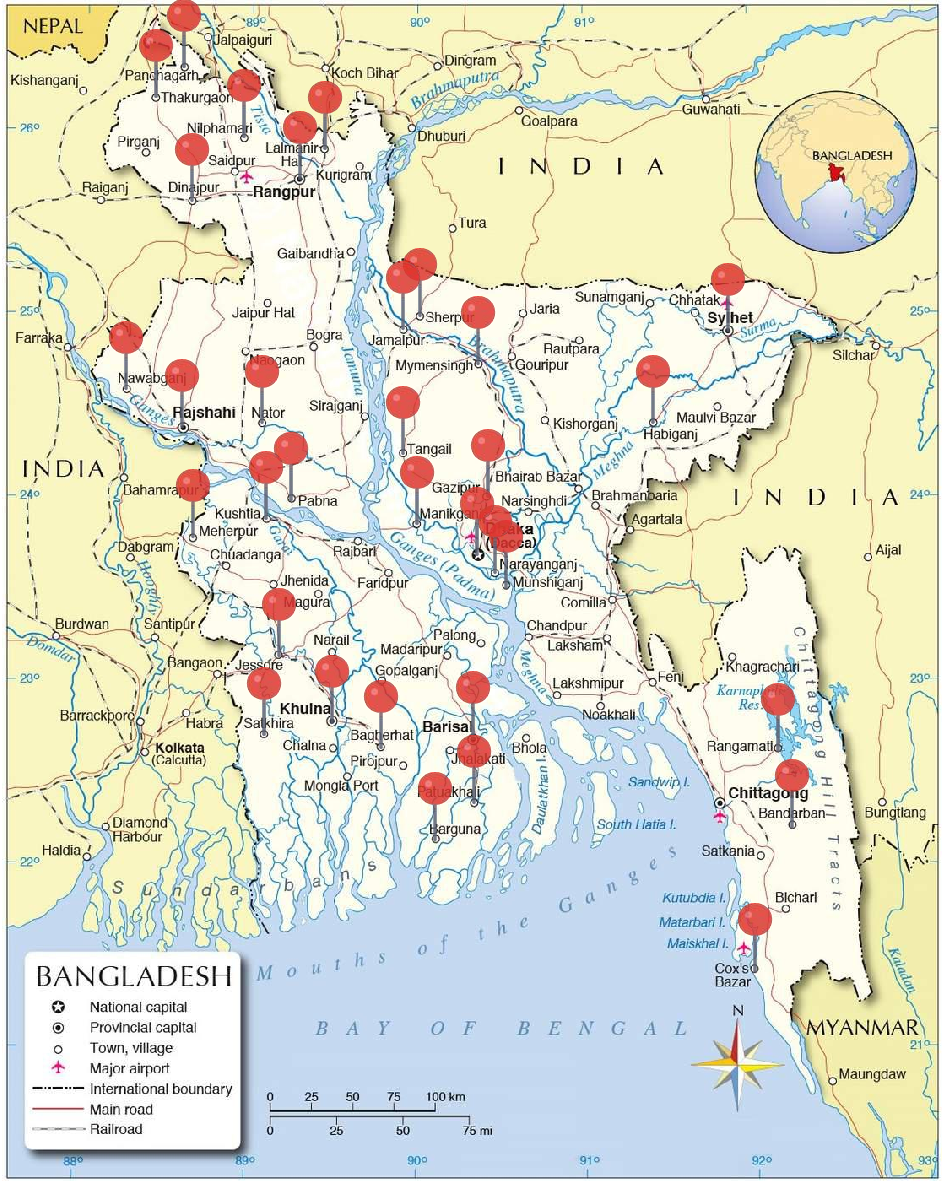
\includegraphics[width=0.99\linewidth]{PinnedMap-crop}}
\caption{Map of Bangladesh with pins indicating locations where workshops have been held.}
\label{fig:map}
\end{figure}

%------------------------------------------------

\begin{figure*}[t!]
    \centering
    \begin{subfigure}[]{0.46\textwidth}
        \centering
        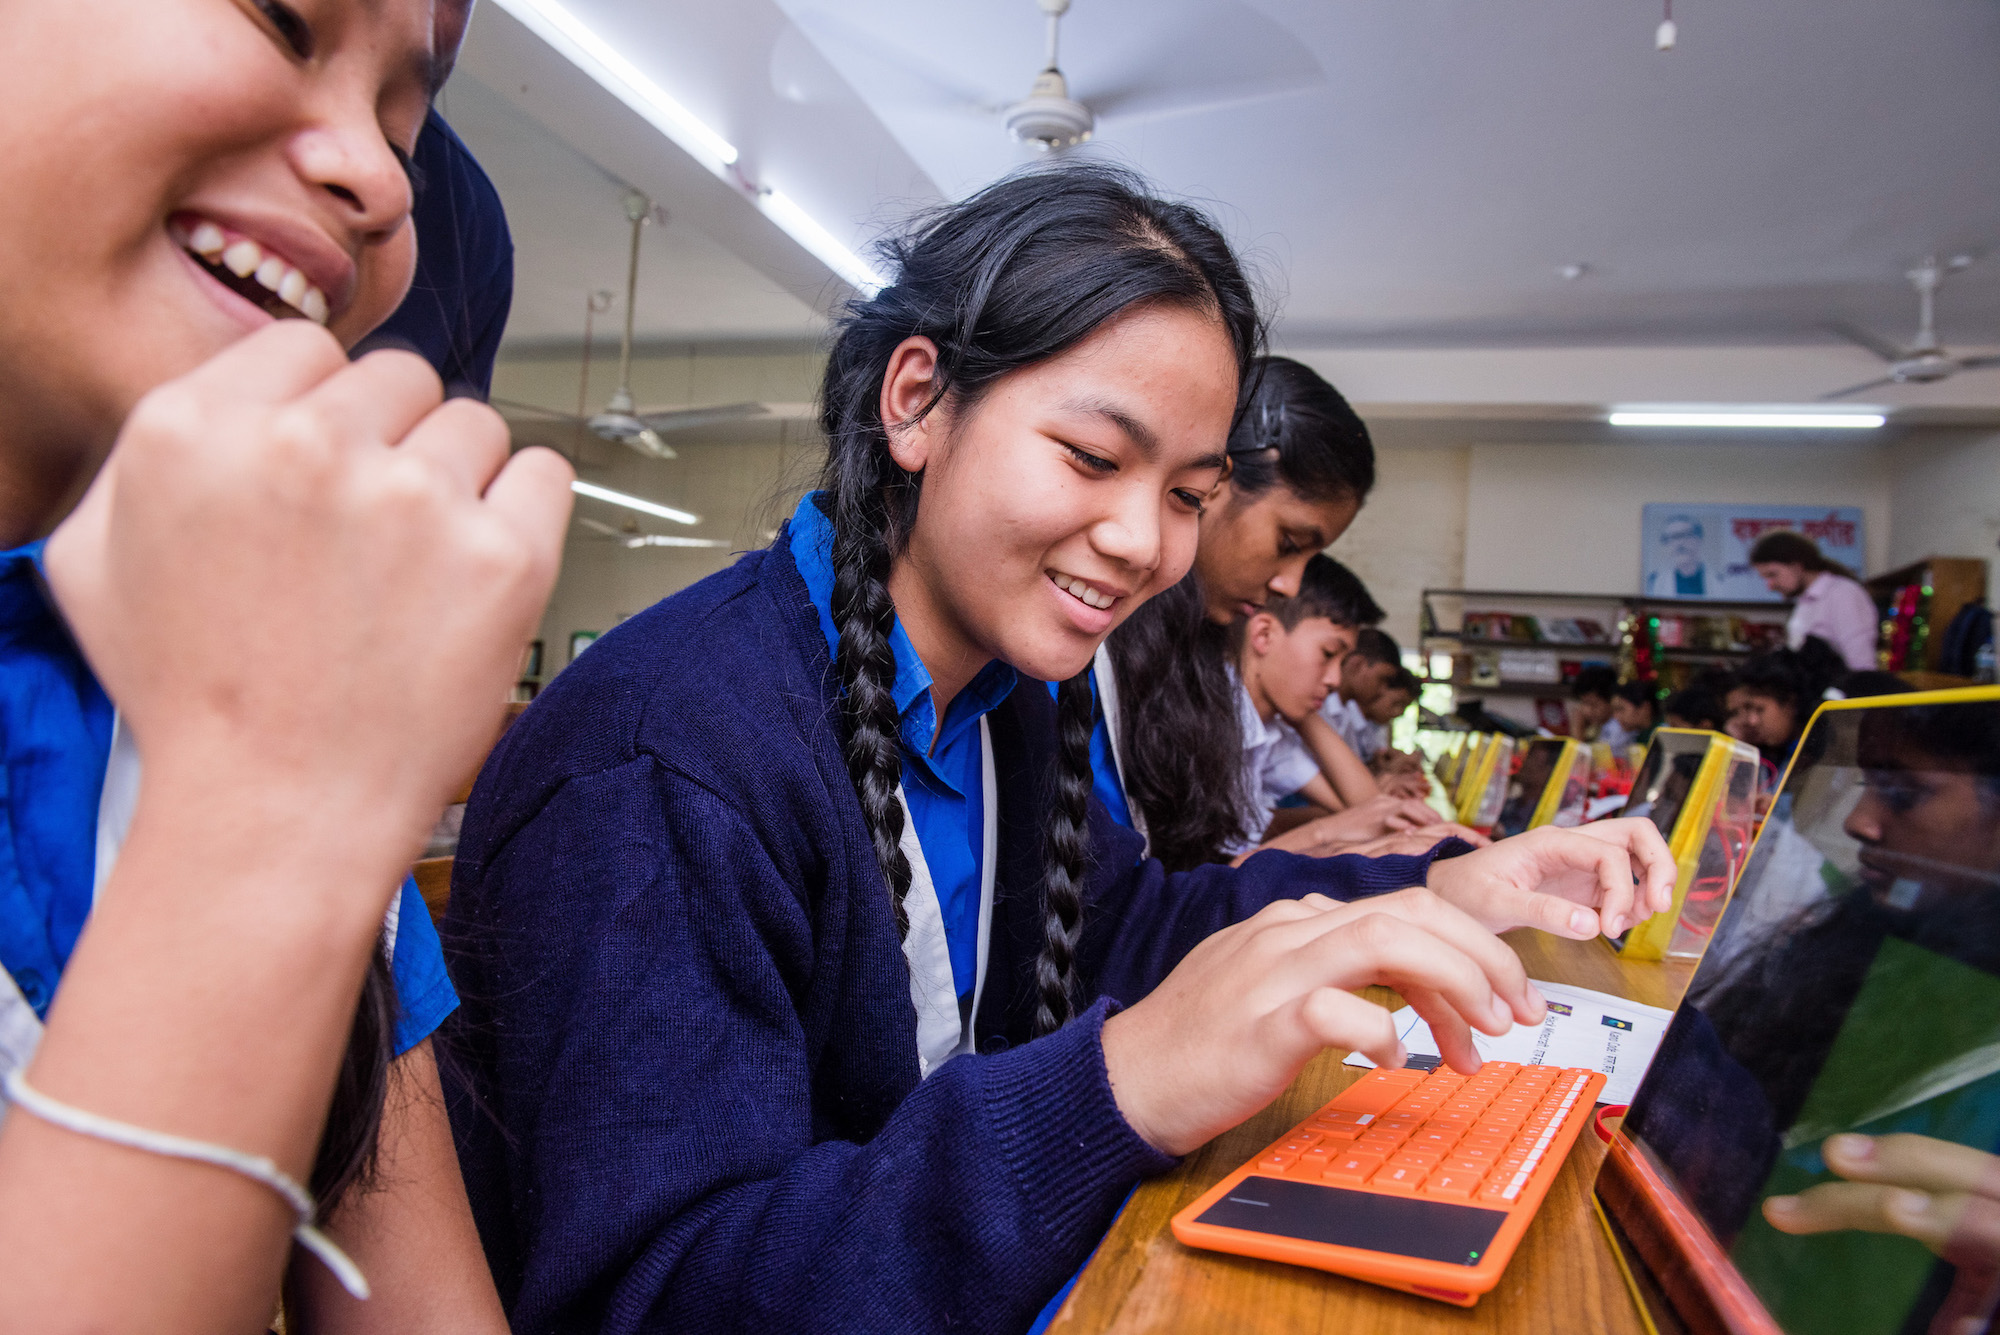
\includegraphics[width=1.0\textwidth]{rang2}
    \end{subfigure}
    \begin{subfigure}[]{0.46\textwidth}
        \centering
        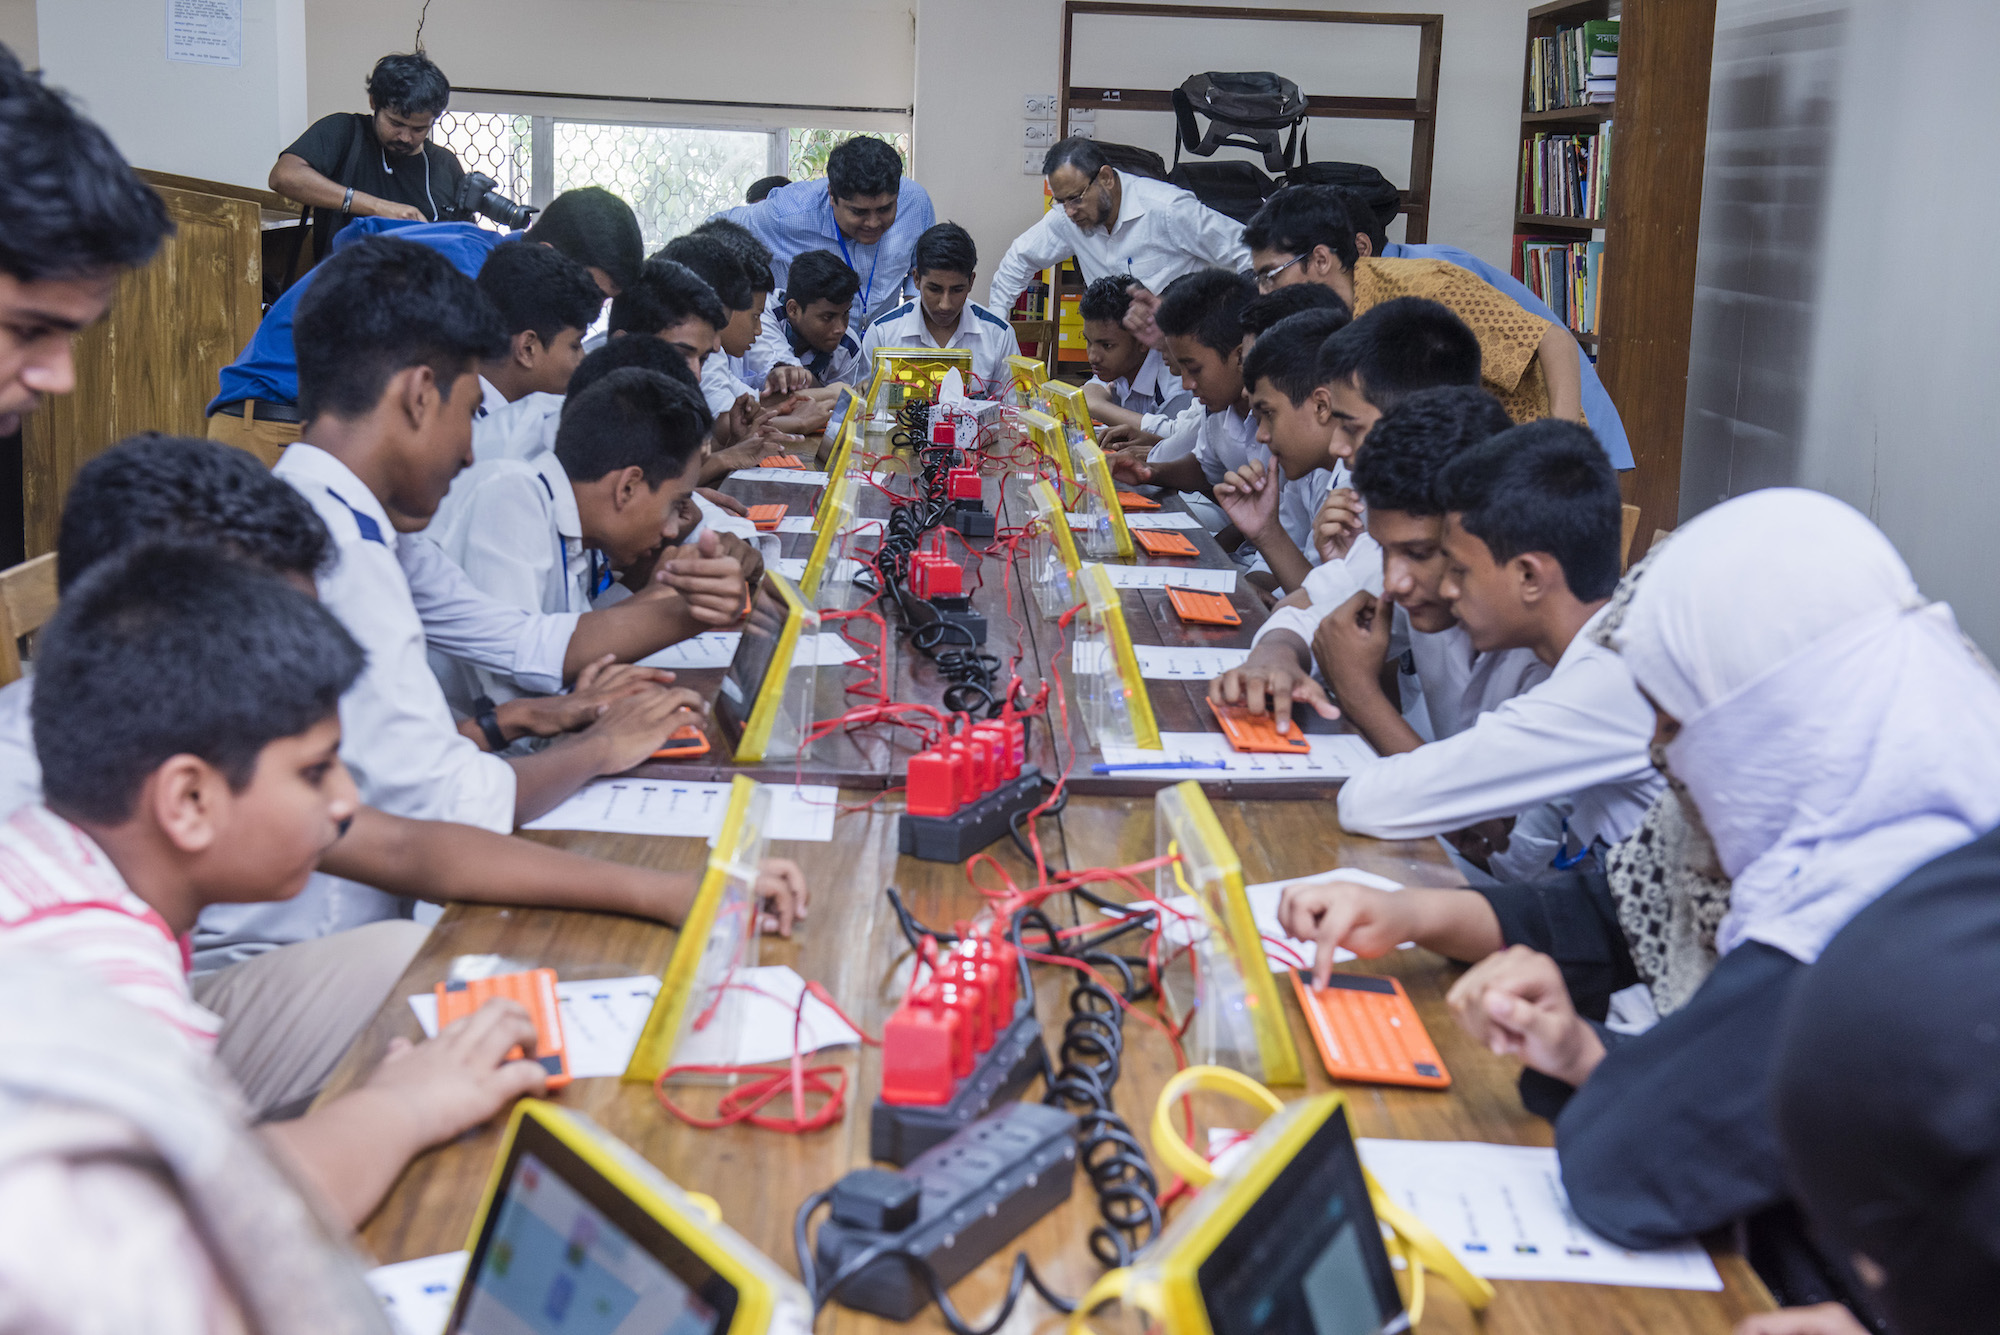
\includegraphics[width=1.0\textwidth]{_TMT7018}
    \end{subfigure}

        \begin{subfigure}[]{0.46\textwidth}
        \centering
        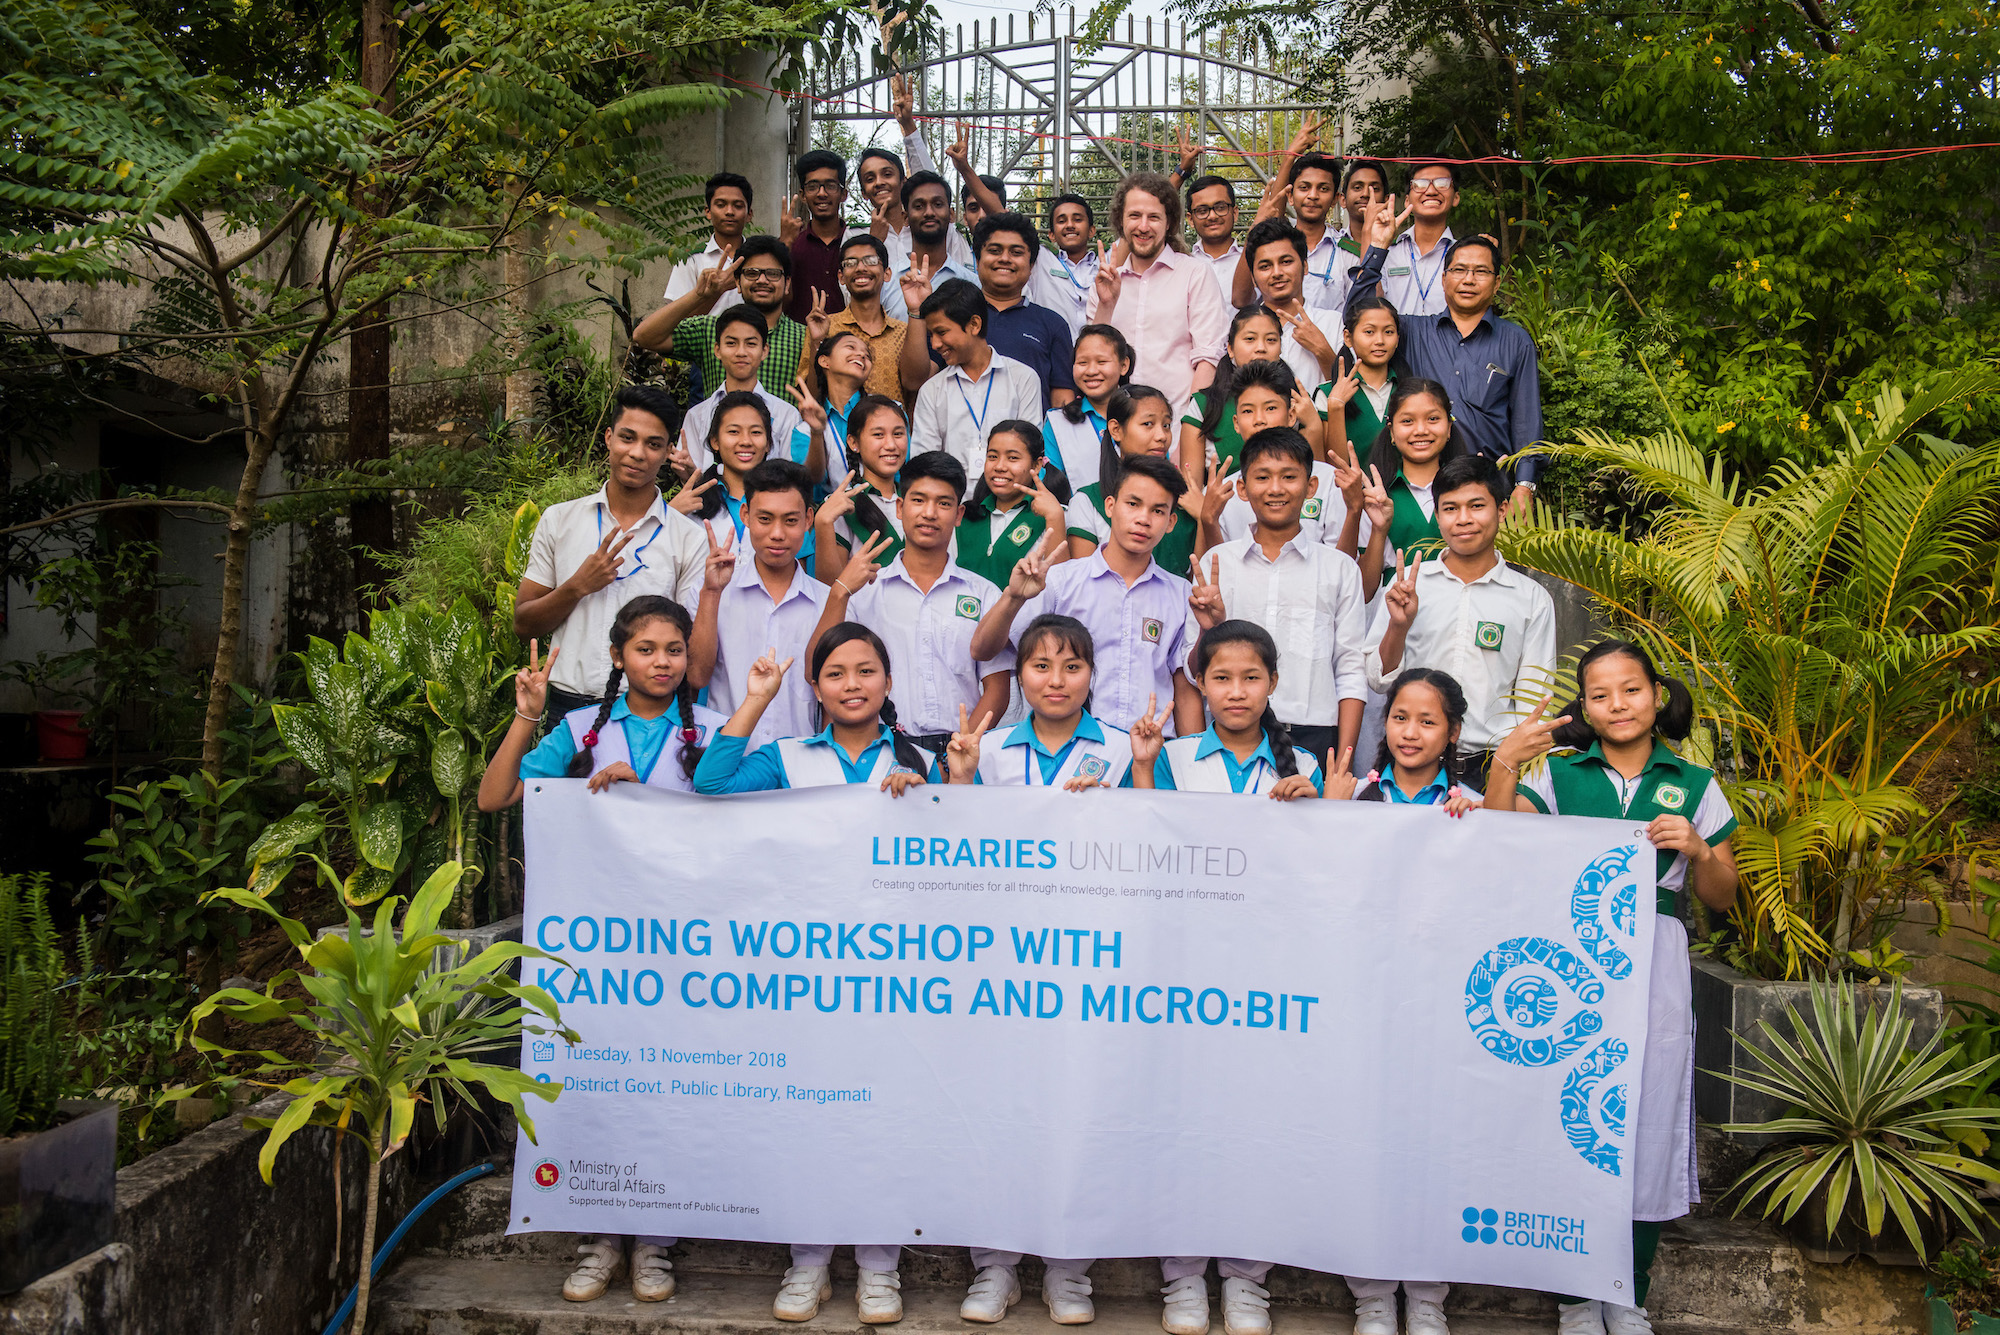
\includegraphics[width=1.0\textwidth]{rang1}
    \end{subfigure}
    \begin{subfigure}[]{0.46\textwidth}
        \centering
        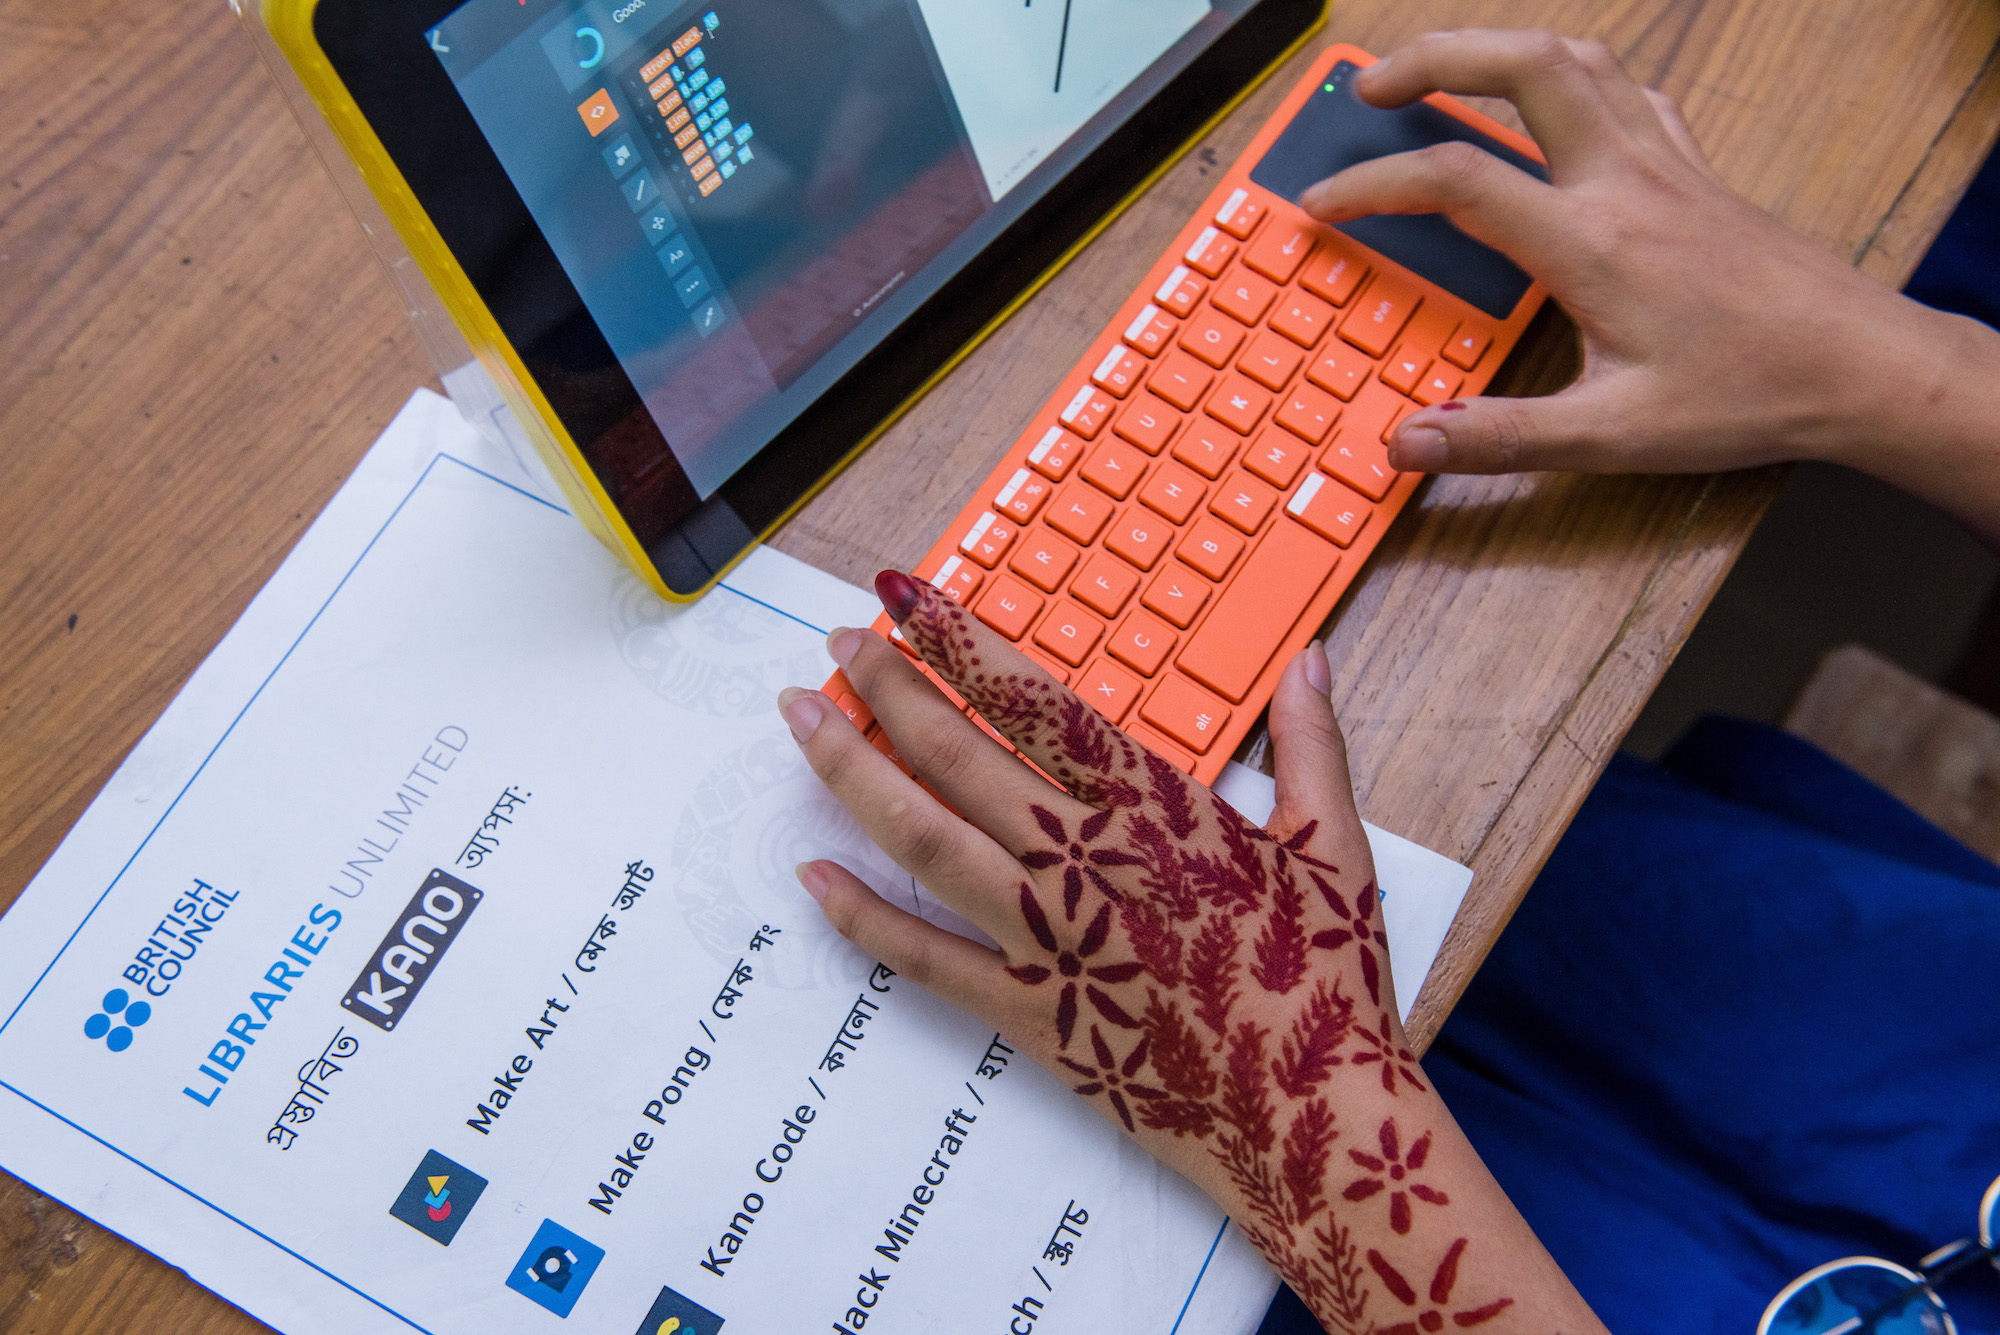
\includegraphics[width=1.0\textwidth]{rang3}
    \end{subfigure}

   
        \begin{subfigure}[]{0.46\textwidth}
        \centering
        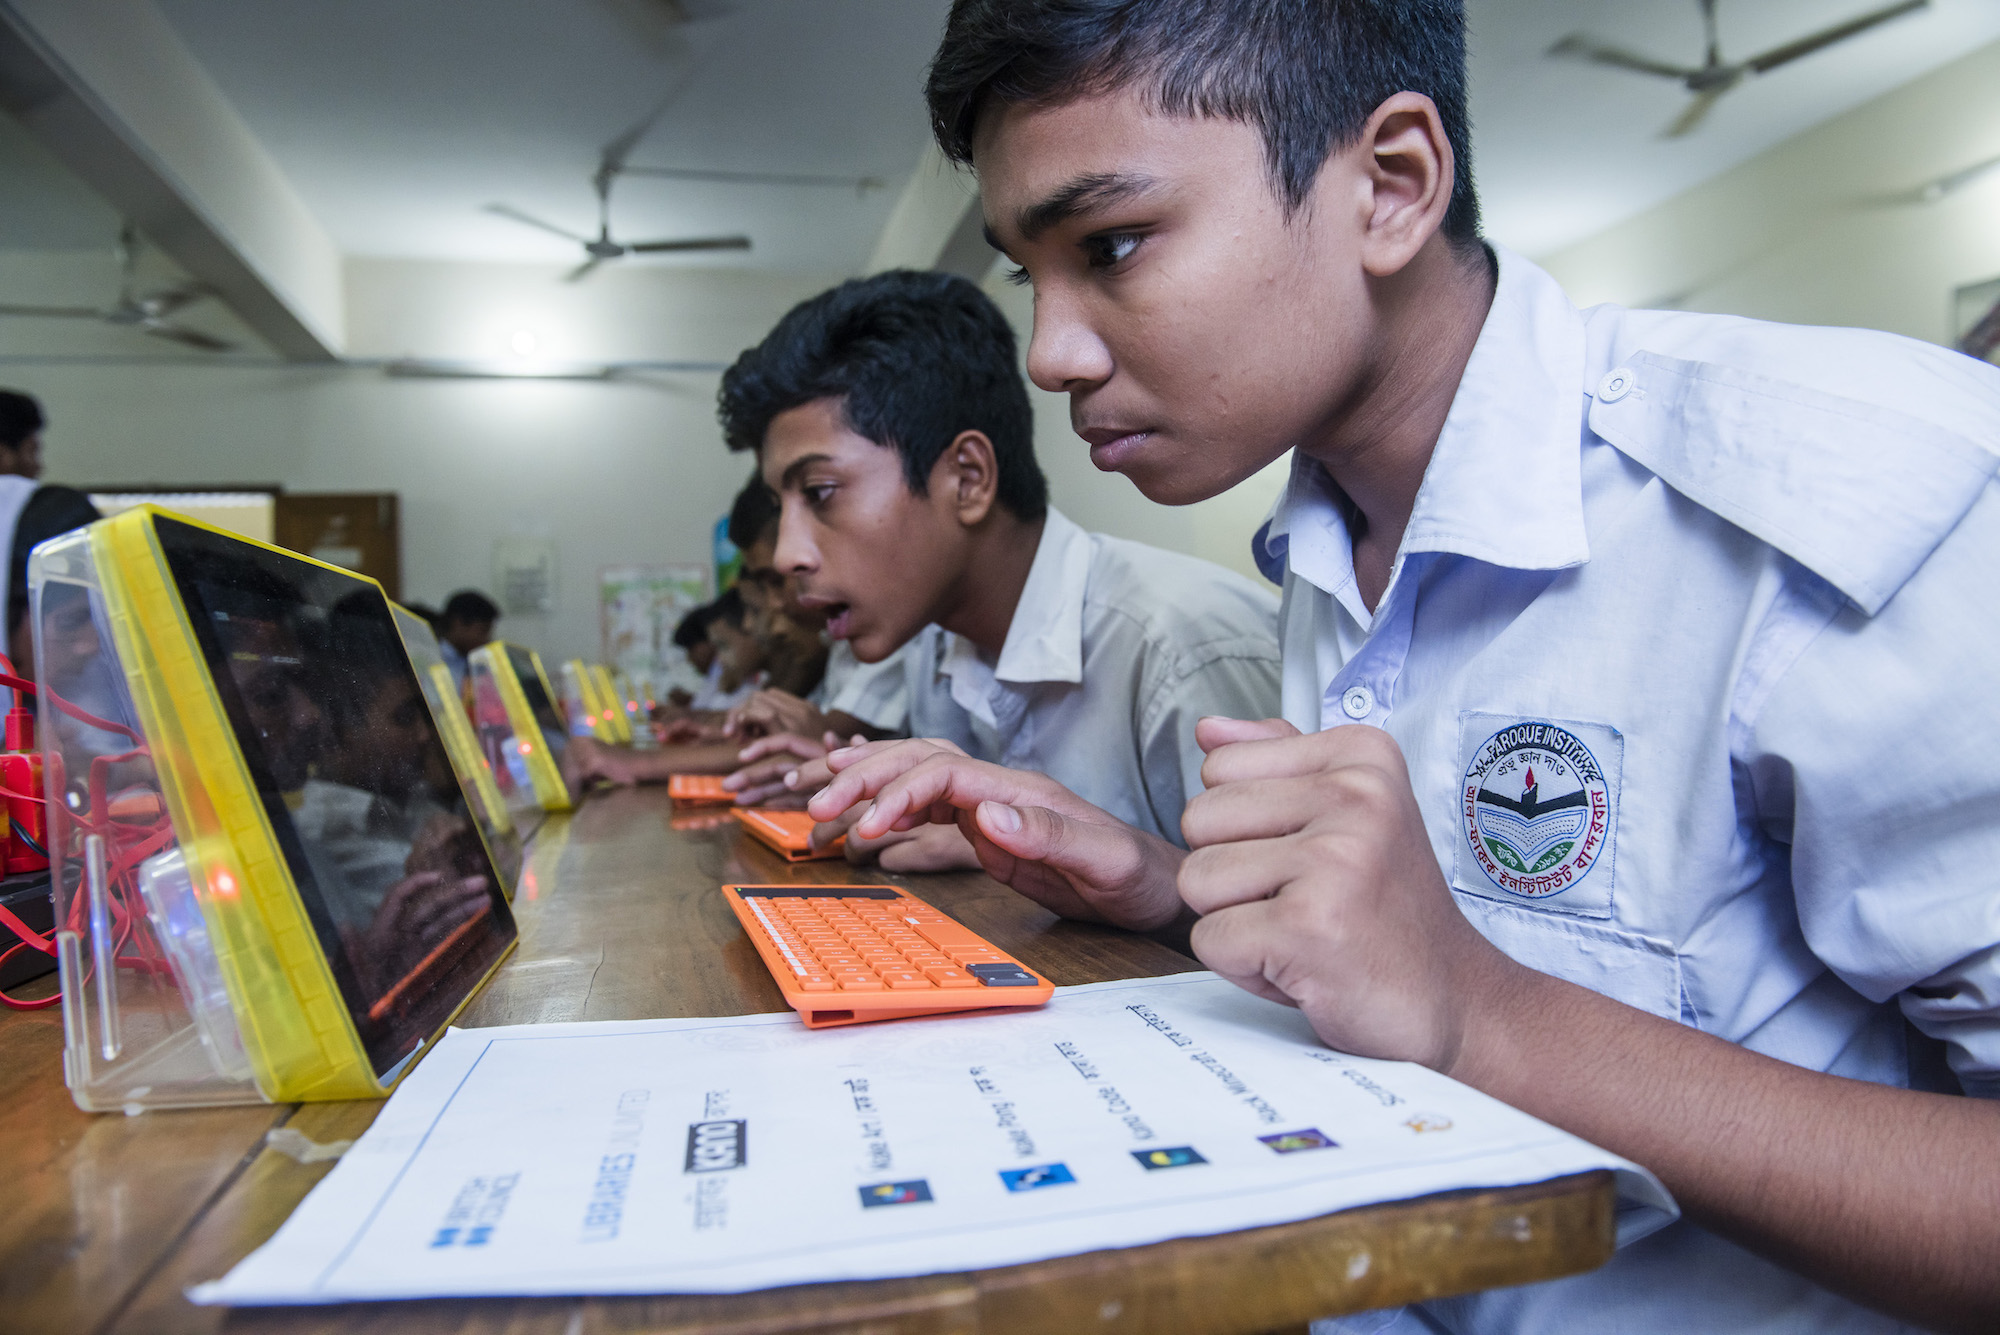
\includegraphics[width=1.0\textwidth]{_TMT4176}
    \end{subfigure}
    \begin{subfigure}[]{0.46\textwidth}
        \centering
        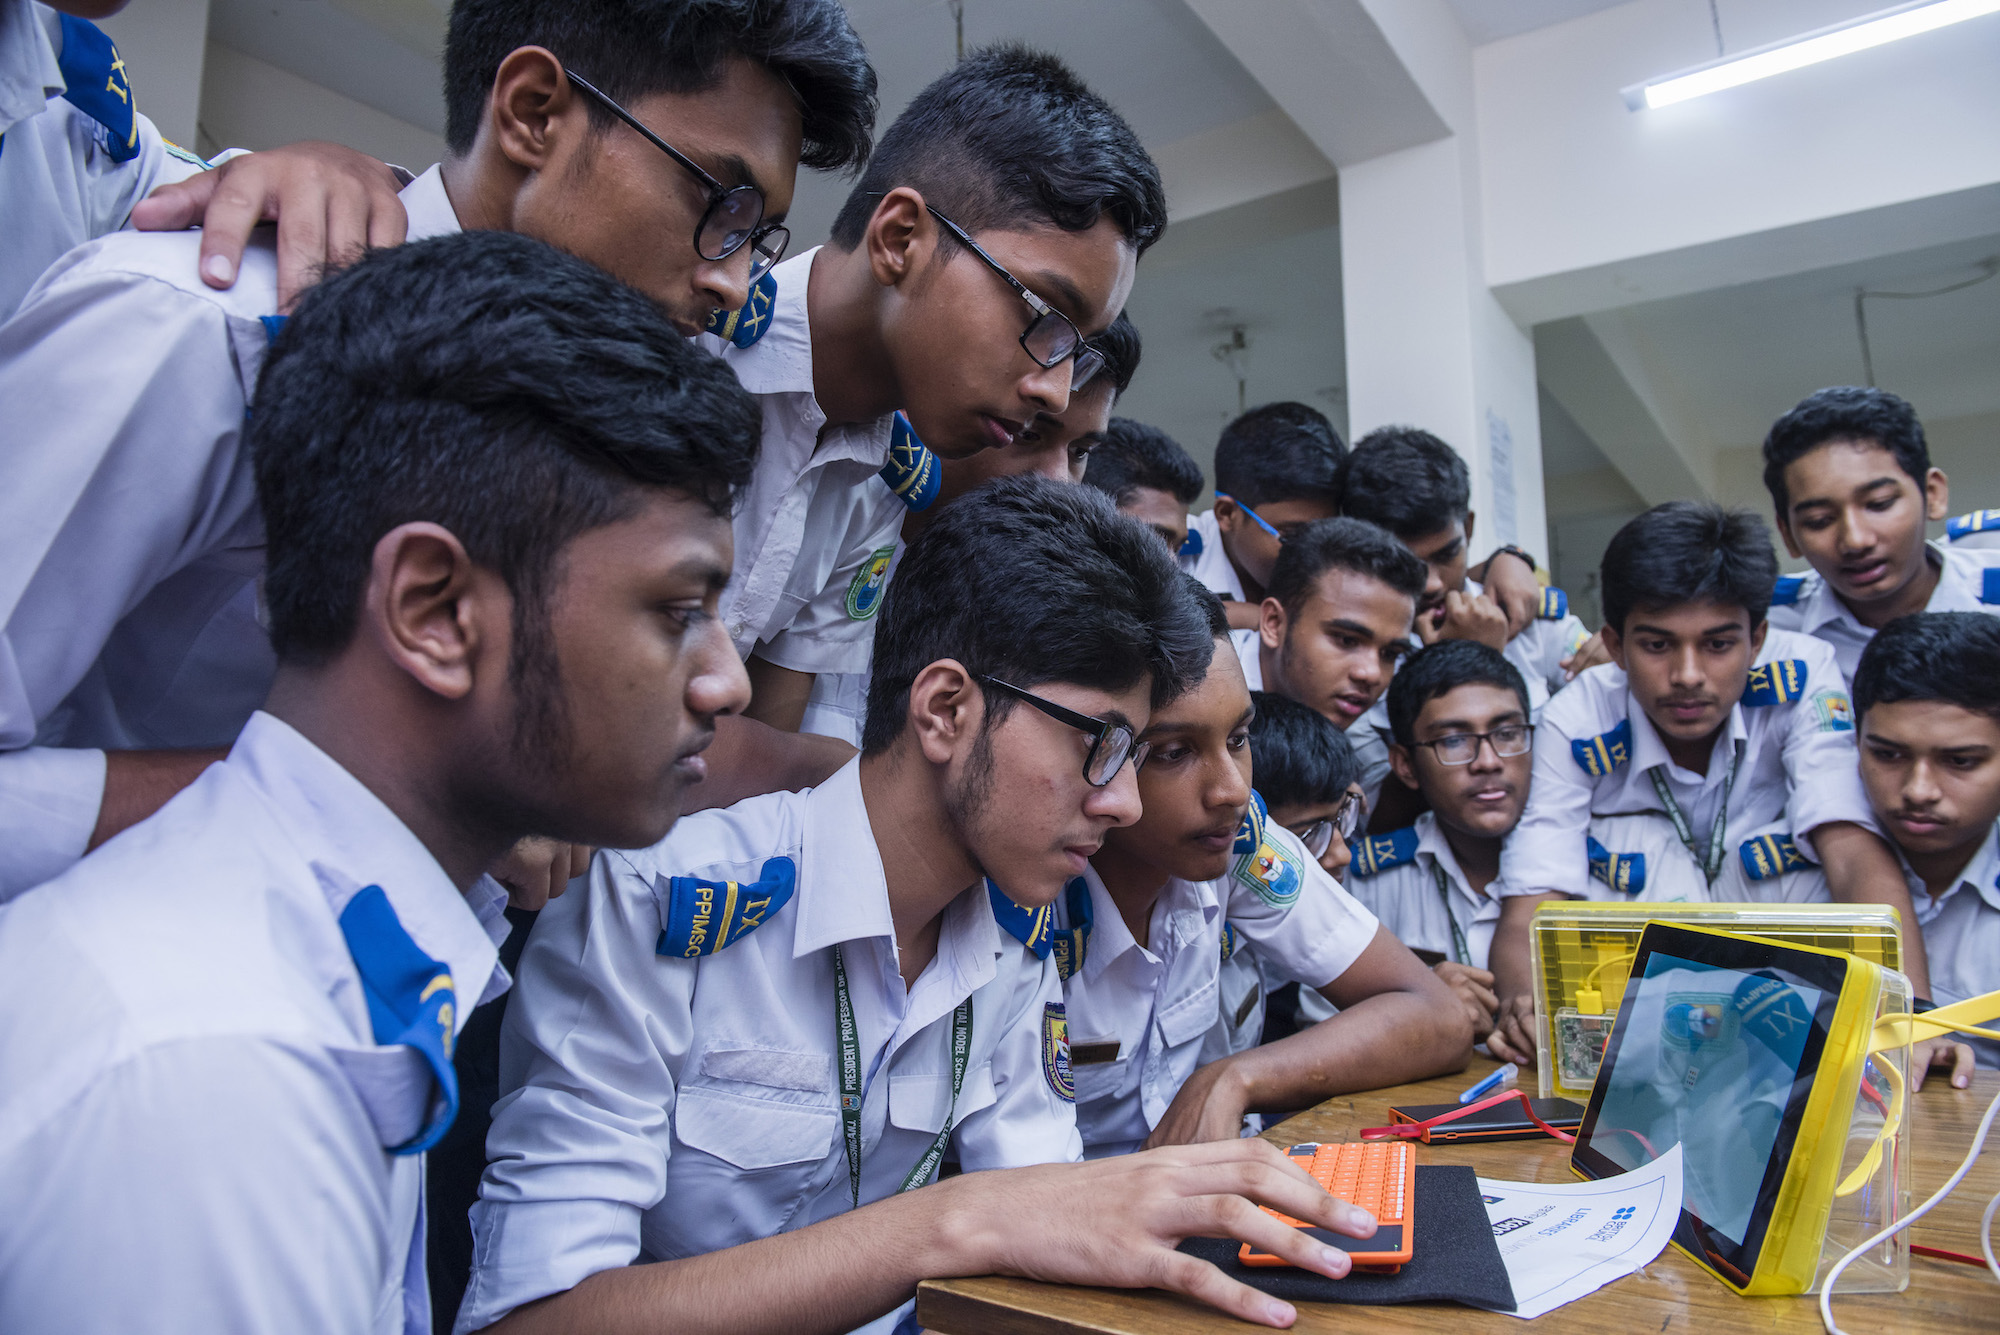
\includegraphics[width=1.0\textwidth]{_TMT7302}
    \end{subfigure}
    
        \begin{subfigure}[]{0.46\textwidth}
        \centering
        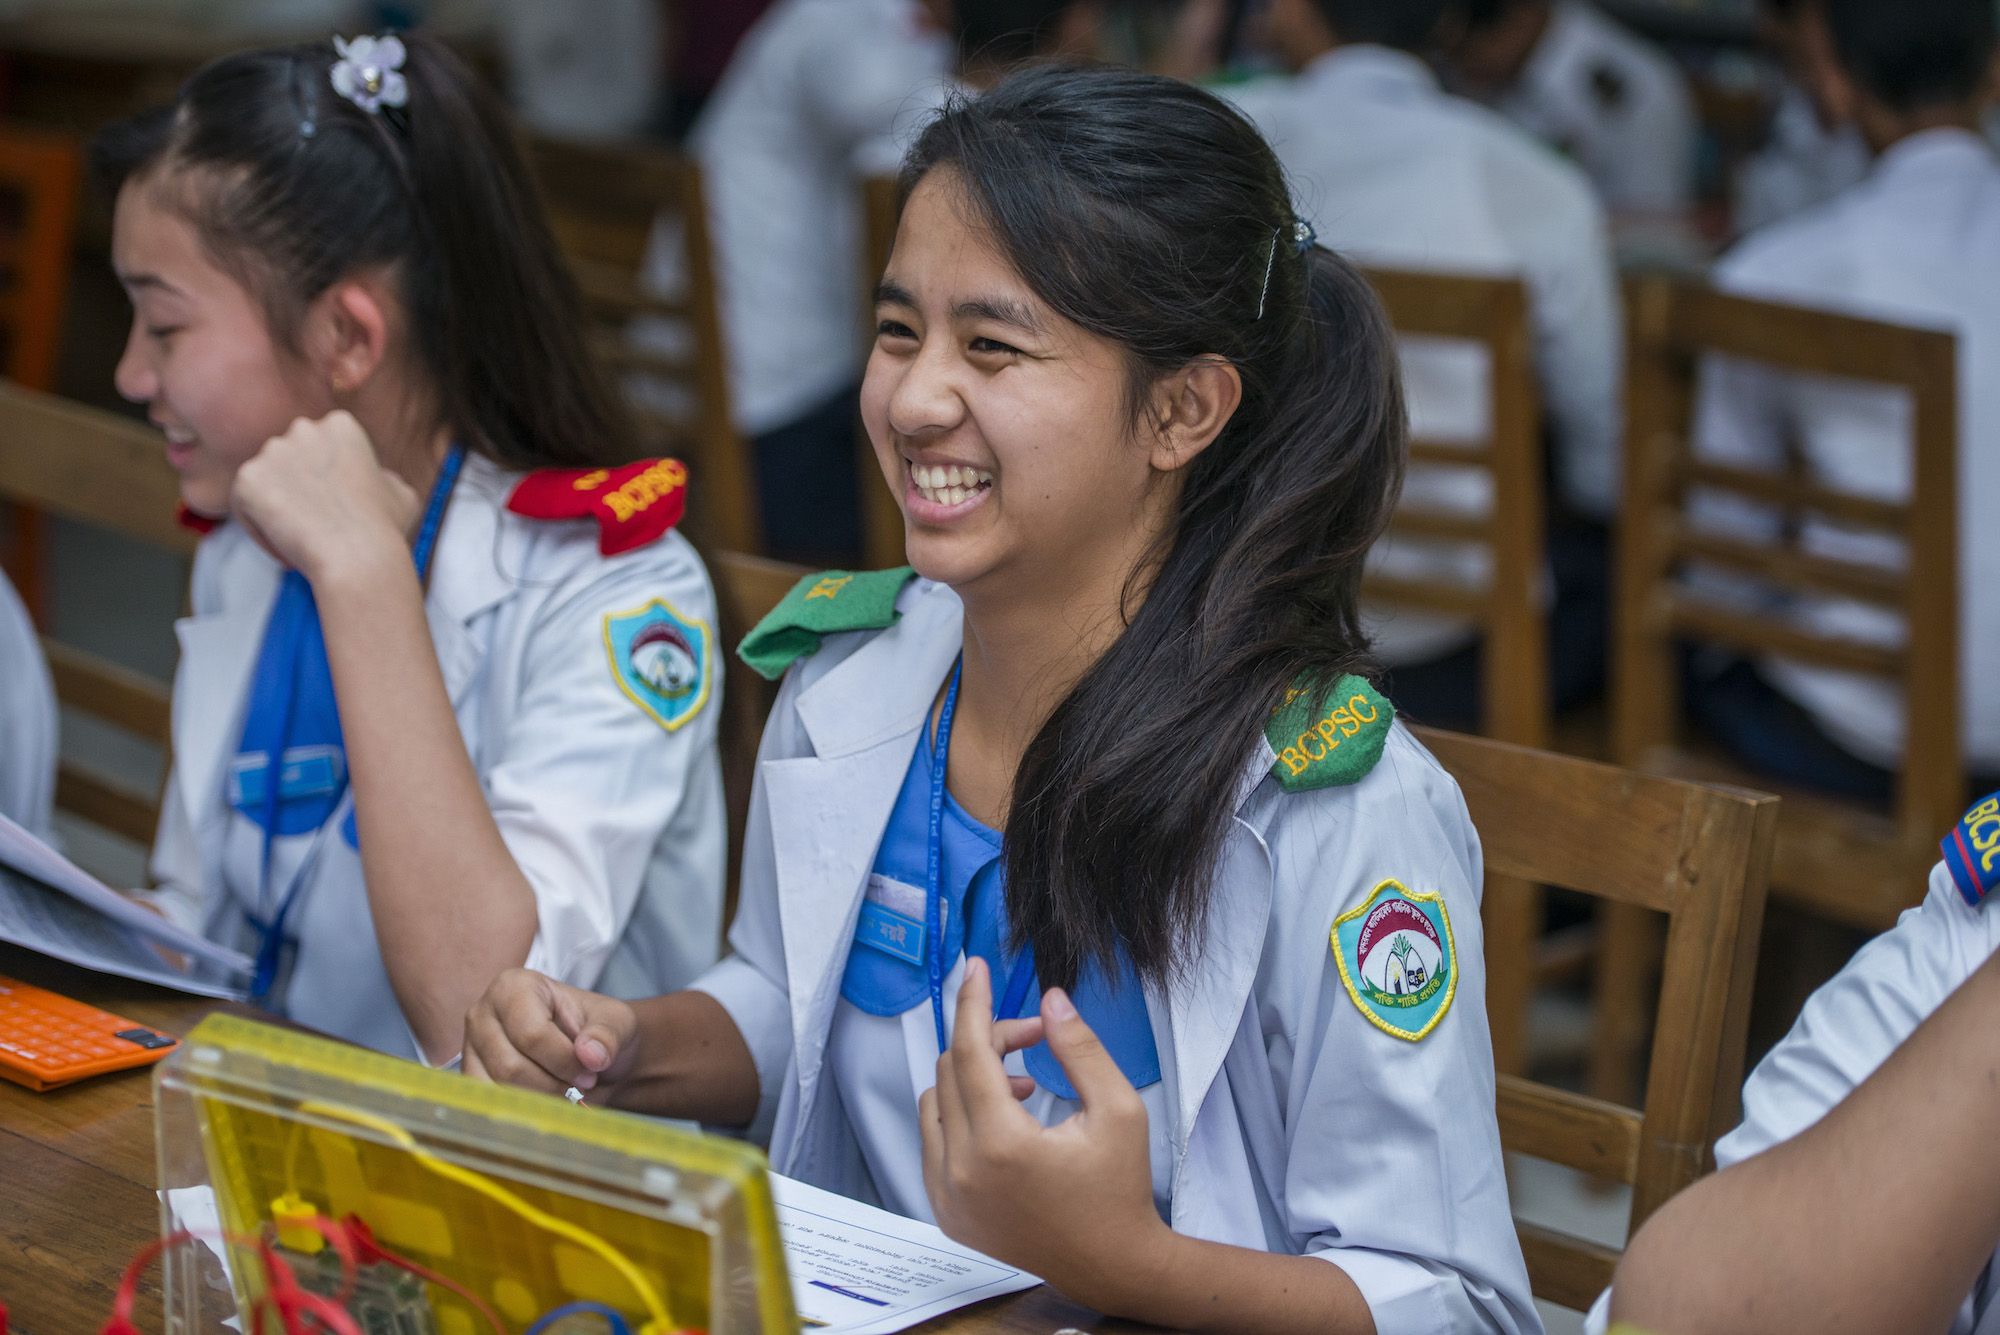
\includegraphics[width=1.0\textwidth]{_TM20868}
    \end{subfigure}
    \begin{subfigure}[]{0.46\textwidth}
        \centering
        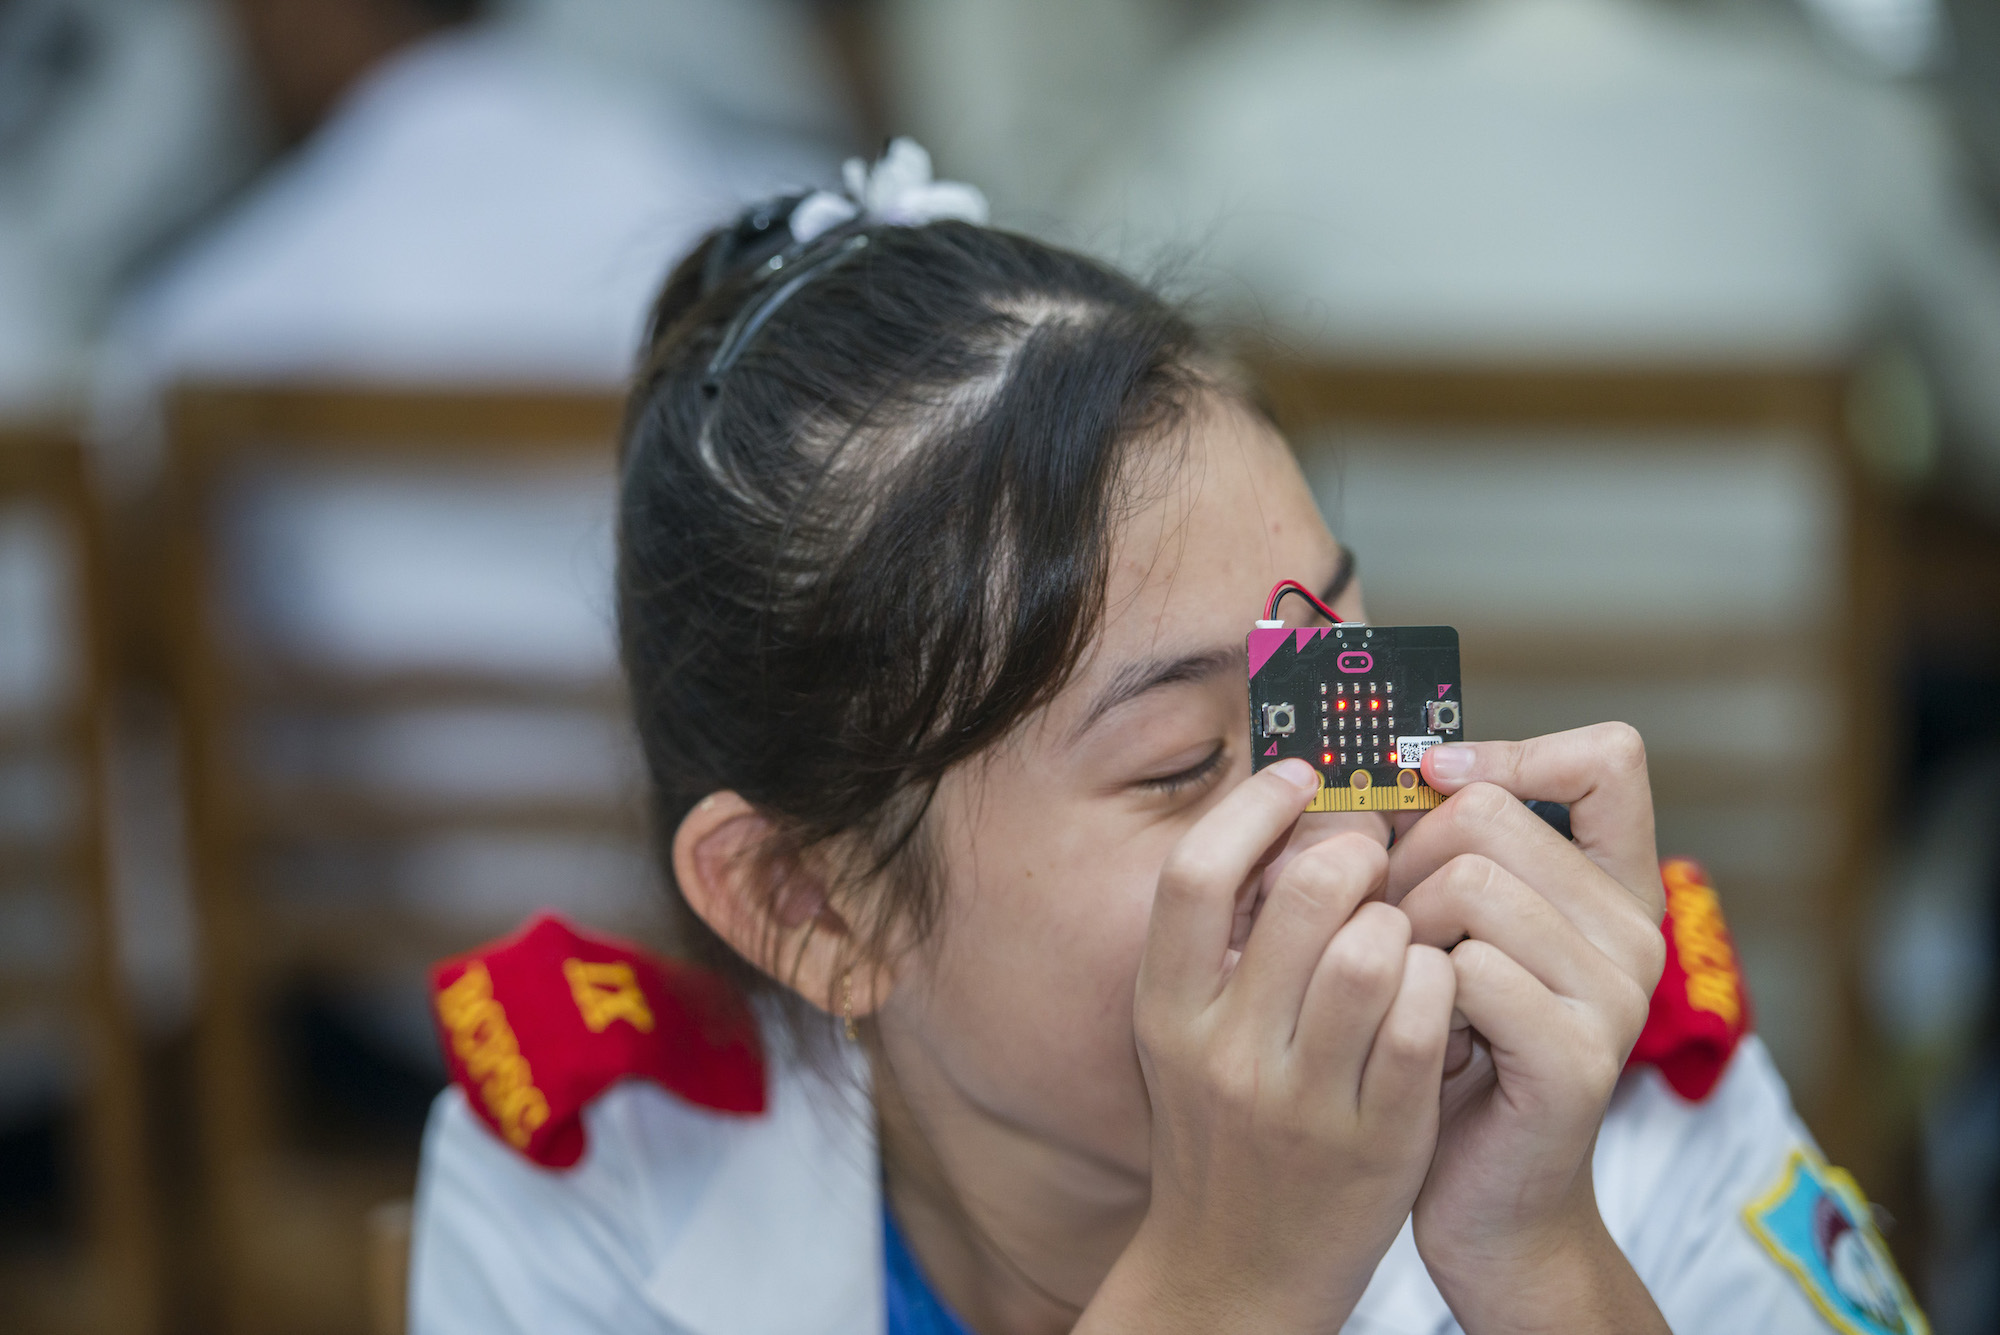
\includegraphics[width=1.0\textwidth]{_TM20980}
    \end{subfigure}    
    \caption{A selection of photos from the Munshiganj, Bandarban and Rangamati library workshops.}
    \label{fig:photos}
\end{figure*}

\newpage
%------------------------------------------------
\subsection{Participant Demographics} % Sub-sub-section

To date the gender distribution of the participants has been 54 per cent male and 46 per cent female (see Figure~\ref{fig:ACgender}). Although near to equality, we would prefer this to be closer to equality. However, invitation of the kids is in the remit of the librarians and the schools have the decision regarding which students to bring.   

\begin{figure}[!htb] % Example image
\center{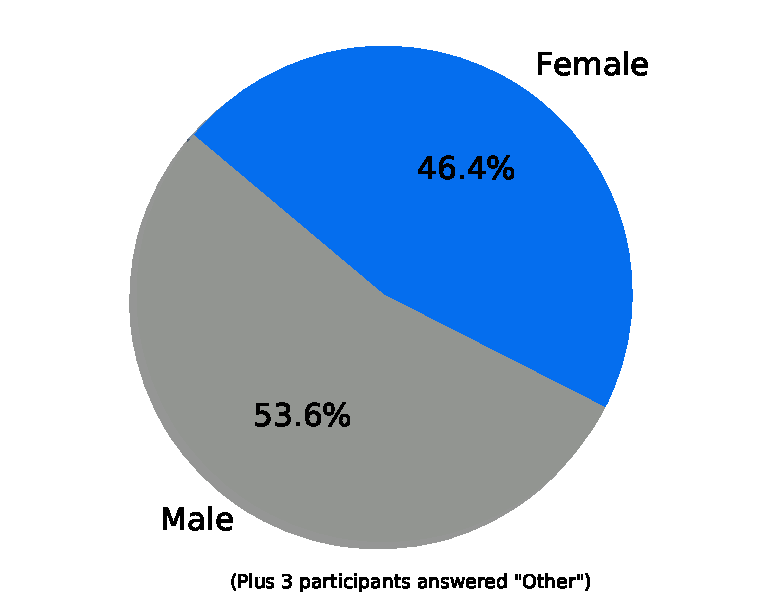
\includegraphics[width=0.6\linewidth]{gender}}
\caption{The gender distribution of participants.}
\label{fig:ACgender}
\end{figure}

%------------------------------------------------

See Figure~\ref{fig:ACage} for the age distribution of participants. The vast majority of participants ($>90$ per cent) have been aged 12 to 16 years old, with an average age of 14 years old. Note that this is by design as we communicate this as the desired age range when planning the workshops.  

\begin{figure}[!htb] % Example image
\center{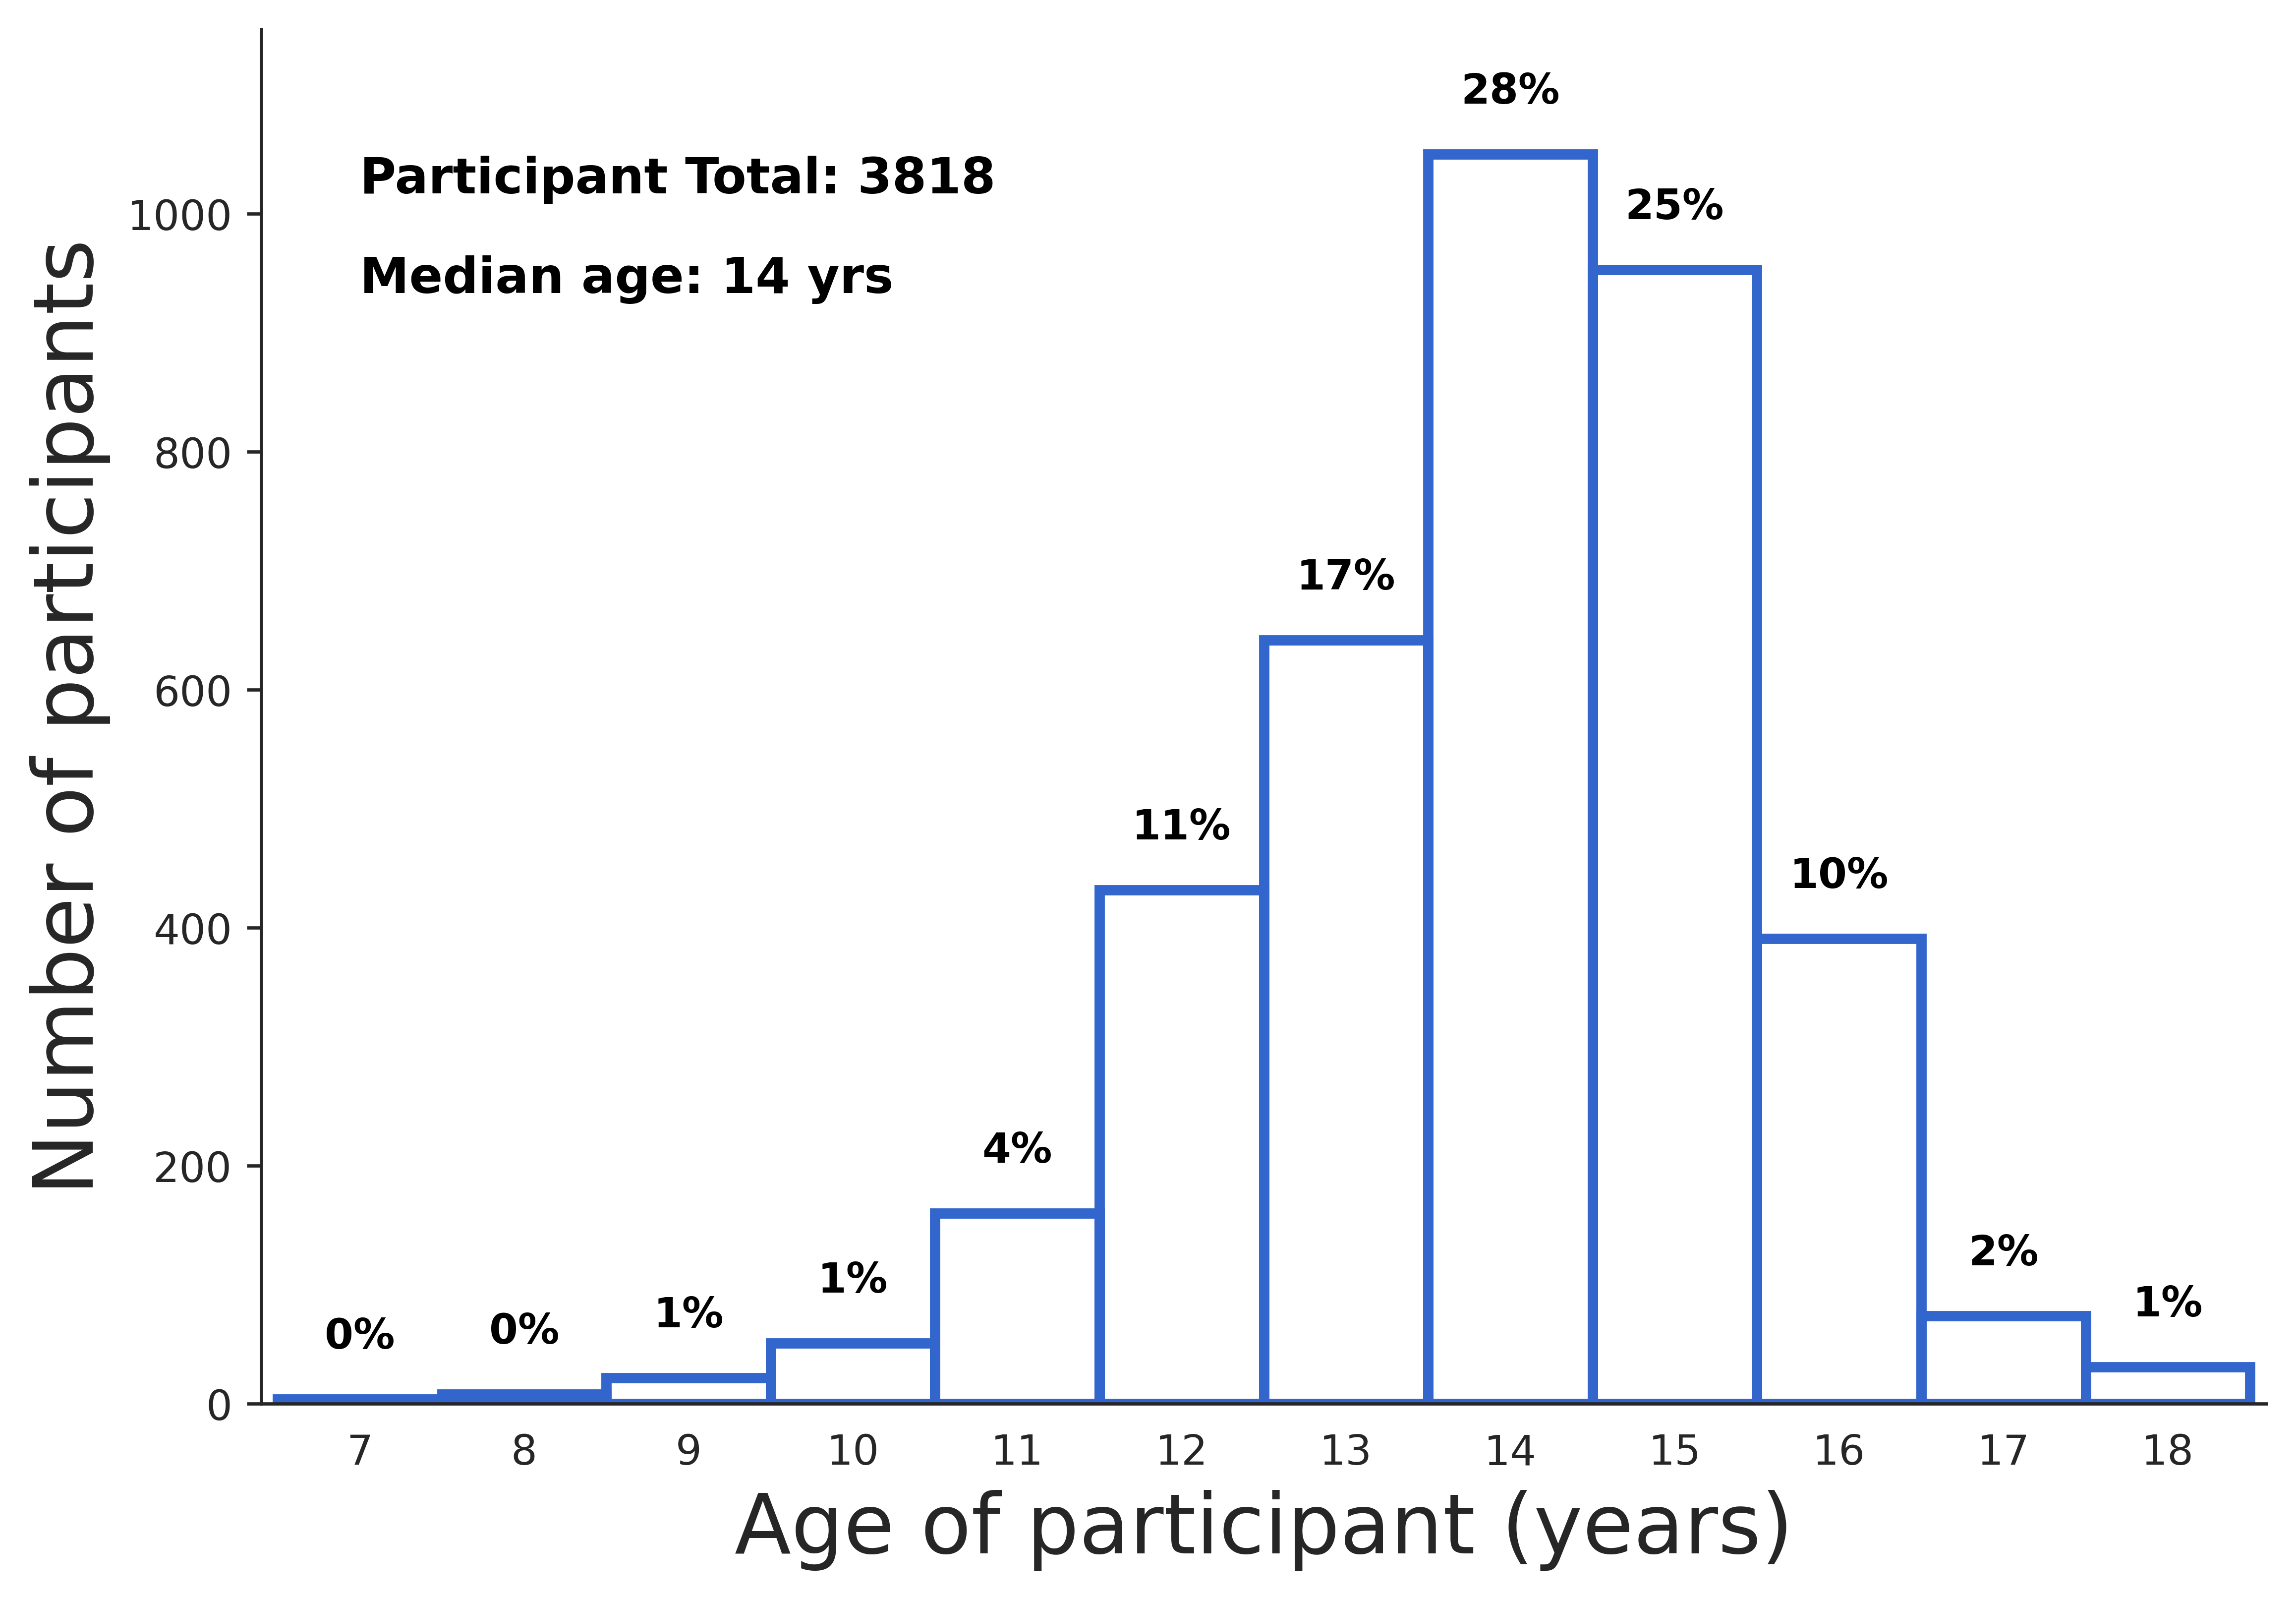
\includegraphics[width=0.65\linewidth]{AgeDistribution}}
\caption{The age distribution of participants.}
\label{fig:ACage}
\end{figure}

%----------------------------------------------------------------------------------------
%	MAJOR SECTION 1
%----------------------------------------------------------------------------------------

\goodbreak
\section{Feedback Results} % Major section
This section will explore the results of the feedback collected:

Figure~\ref{fig:quotes} provides a selection of written comments from participants. Then Figures~\ref{fig:ACworkshopexp}--\ref{fig:challenge} graphically illustrate feedback results; this includes their perceived confidence in their ability to do coding, how interested they are in doing coding, how important they believe coding is, their experience of the workshop, and how often the participants use computers and public libraries, with breakdowns by gender. 


\subsection{Summary of key findings:}
\begin{itemize}
\item We asked the participants to rate their overall experience of the workshop: 77 per cent said it was very good and less than one per cent said it was bad (see Figure~\ref{fig:ACworkshopexp}).

\item There is a clear increase in confidence for the participants and their perceived ability to do coding. Prior to the workshop only 29 per cent felt they were able to do coding, 39 per cent of participants answered that were unable to do coding and 32 per cent didn't know whether they could. Following the workshop, 74 per cent felt they were able to do coding, with 14 per cent unsure and 12 per cent still not confident in their ability (see Figure~\ref{fig:ACcandocoding}). 

\item The number of participants who are interested in coding was increased by the workshop, despite an initial high level of interest prior to the workshop already. The proportion of participants who are very interested in doing coding increased from 65 per cent before the workshop to 69 per cent after. And the proportion of participants who were not interested in learning coding or were unsure decreased from seven to four per cent (see Figure~\ref{fig:ACcodinginterest}). 

\item The workshops increased the perception of the participants in how important coding is to their lives. Prior to the workshop 18 per cent of participants felt coding was unimportant to their lives, or were unsure. After the workshop this reduced to only three per cent. The number who answered that coding was very important increased from 52 per cent to 69 per cent (see Figure~\ref{fig:ACcodingimportance}). 

%\item The majority of participants have never done coding before, but 95 per cent said they would be interested in learning more coding in the future.
\item When asked, 41 per cent of participants said they do not have regular access to a computer at home or at school. This highlights the important role libraries can play in providing IT access to citizens who otherwise would not have it (see Figure~\ref{fig:itaccess}).

 \item 12 per cent of participants (over 400 individuals) said the workshop was their first time using a computer. This figure is higher for the female participants (15 per cent, compared to nine per cent of males; see Figure~\ref{fig:itusefreq}). This is despite a similar proportion of respondents of both genders having access to a computer at home or school (see Figure~\ref{fig:itaccess}).
 
\item Introducing new services has the potential to attract new users. When asked, 42 per cent of participants said the workshop was their first time using the public library (see Figure~\ref{fig:libusefreq}), so the workshops are introducing young people to their library. When asked whether they are more likely to visit the library more often if activities like this are offered, 88 per cent said yes, 11 per cent said maybe and less than one per cent said no (see Figure~\ref{fig:libraryvisitactivities}). And also when asked whether thay are more likely to visit the library if the devices are made avaible then 84 per cent said yes (see Figure~\ref{fig:libraryvisitdevices}).

\item Girls are much less likely to be have used, and regularly be using, the libraries than boys. 48 per cent of girls said they had never used the library before, compared to 38 per cent of boys (see Figure~\ref{fig:libusefreq}). And only three per cent of girls said they very regularly use the library (i.e. multiple times a week), compared to eight per cent of boys. This is despite a higher proportion of girls expressing interest in visiting the library (with 57 per cent of girls saying they are very interested in visiting the library compared with 40 per cent of boys; see Figure~\ref{fig:libvisitinterest}). 
\end{itemize}
  
\subsection{Revision of questionnaire forms}
It should be noted that a few iterations of the questionnaires have been used to date, with some questions removed and others added. The most substantial revision was the introduction of a pre-workshop questionnaire, introduced in October 2019, in order to measure change before and after the workshop. Prior to this there was a single post--workshop form. As a result of these revisions not all questions have been asked to all participants. In order to illustrate this, the sample size for each of the questions is given in the lower right corner of the corresponding figure. 

\begin{figure*}[t!]
    \centering
        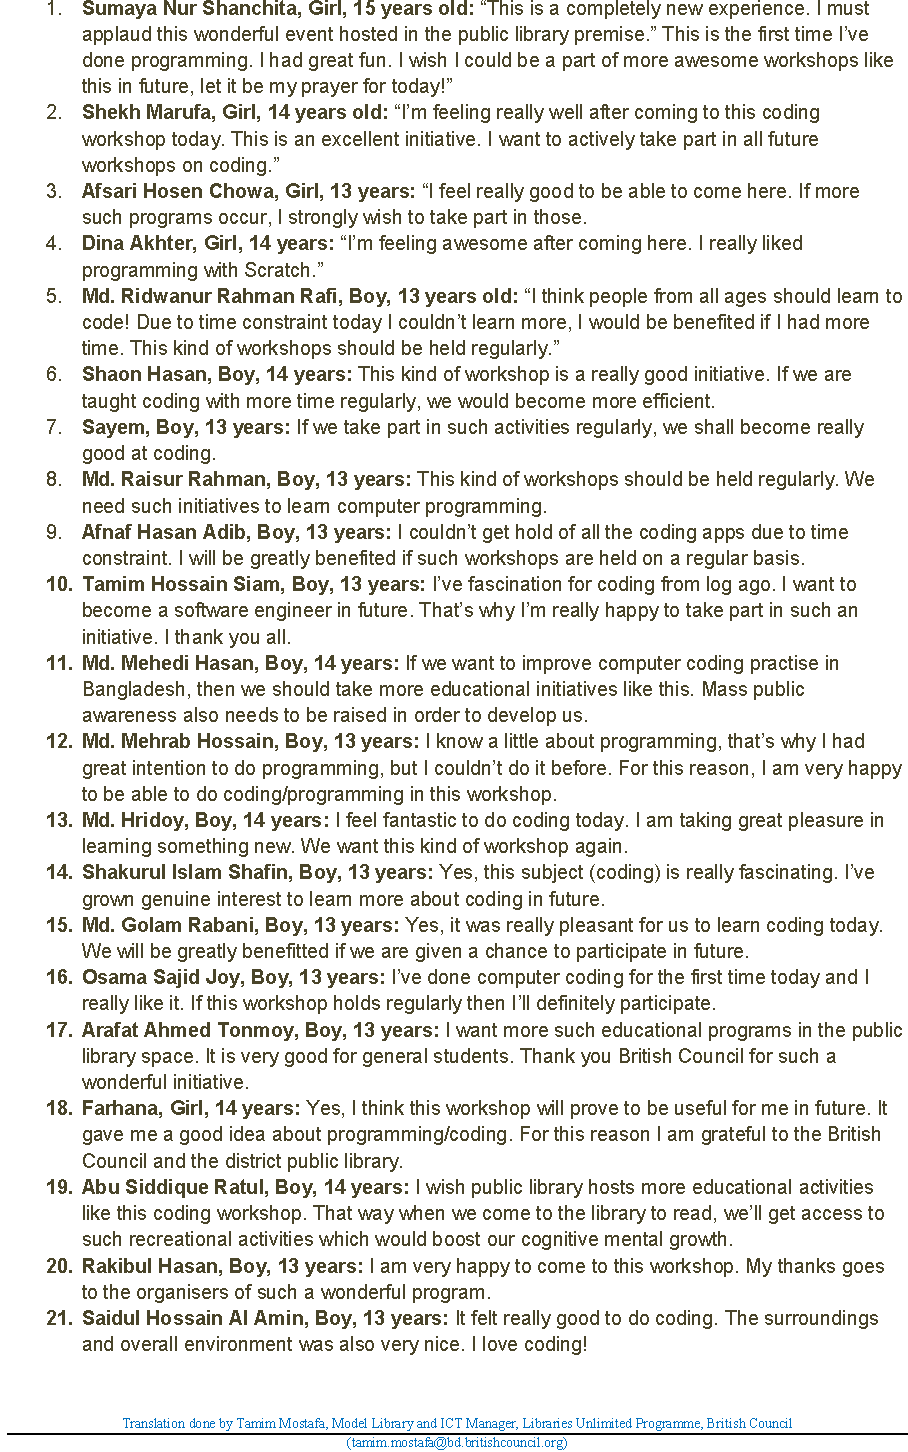
\includegraphics[width=0.85\textwidth]{quotes-crop}
\caption{A selection of written comments collected on the feedback forms.  } 
\label{fig:quotes}
\end{figure*}


\begin{figure*}[t!]
    \centering
        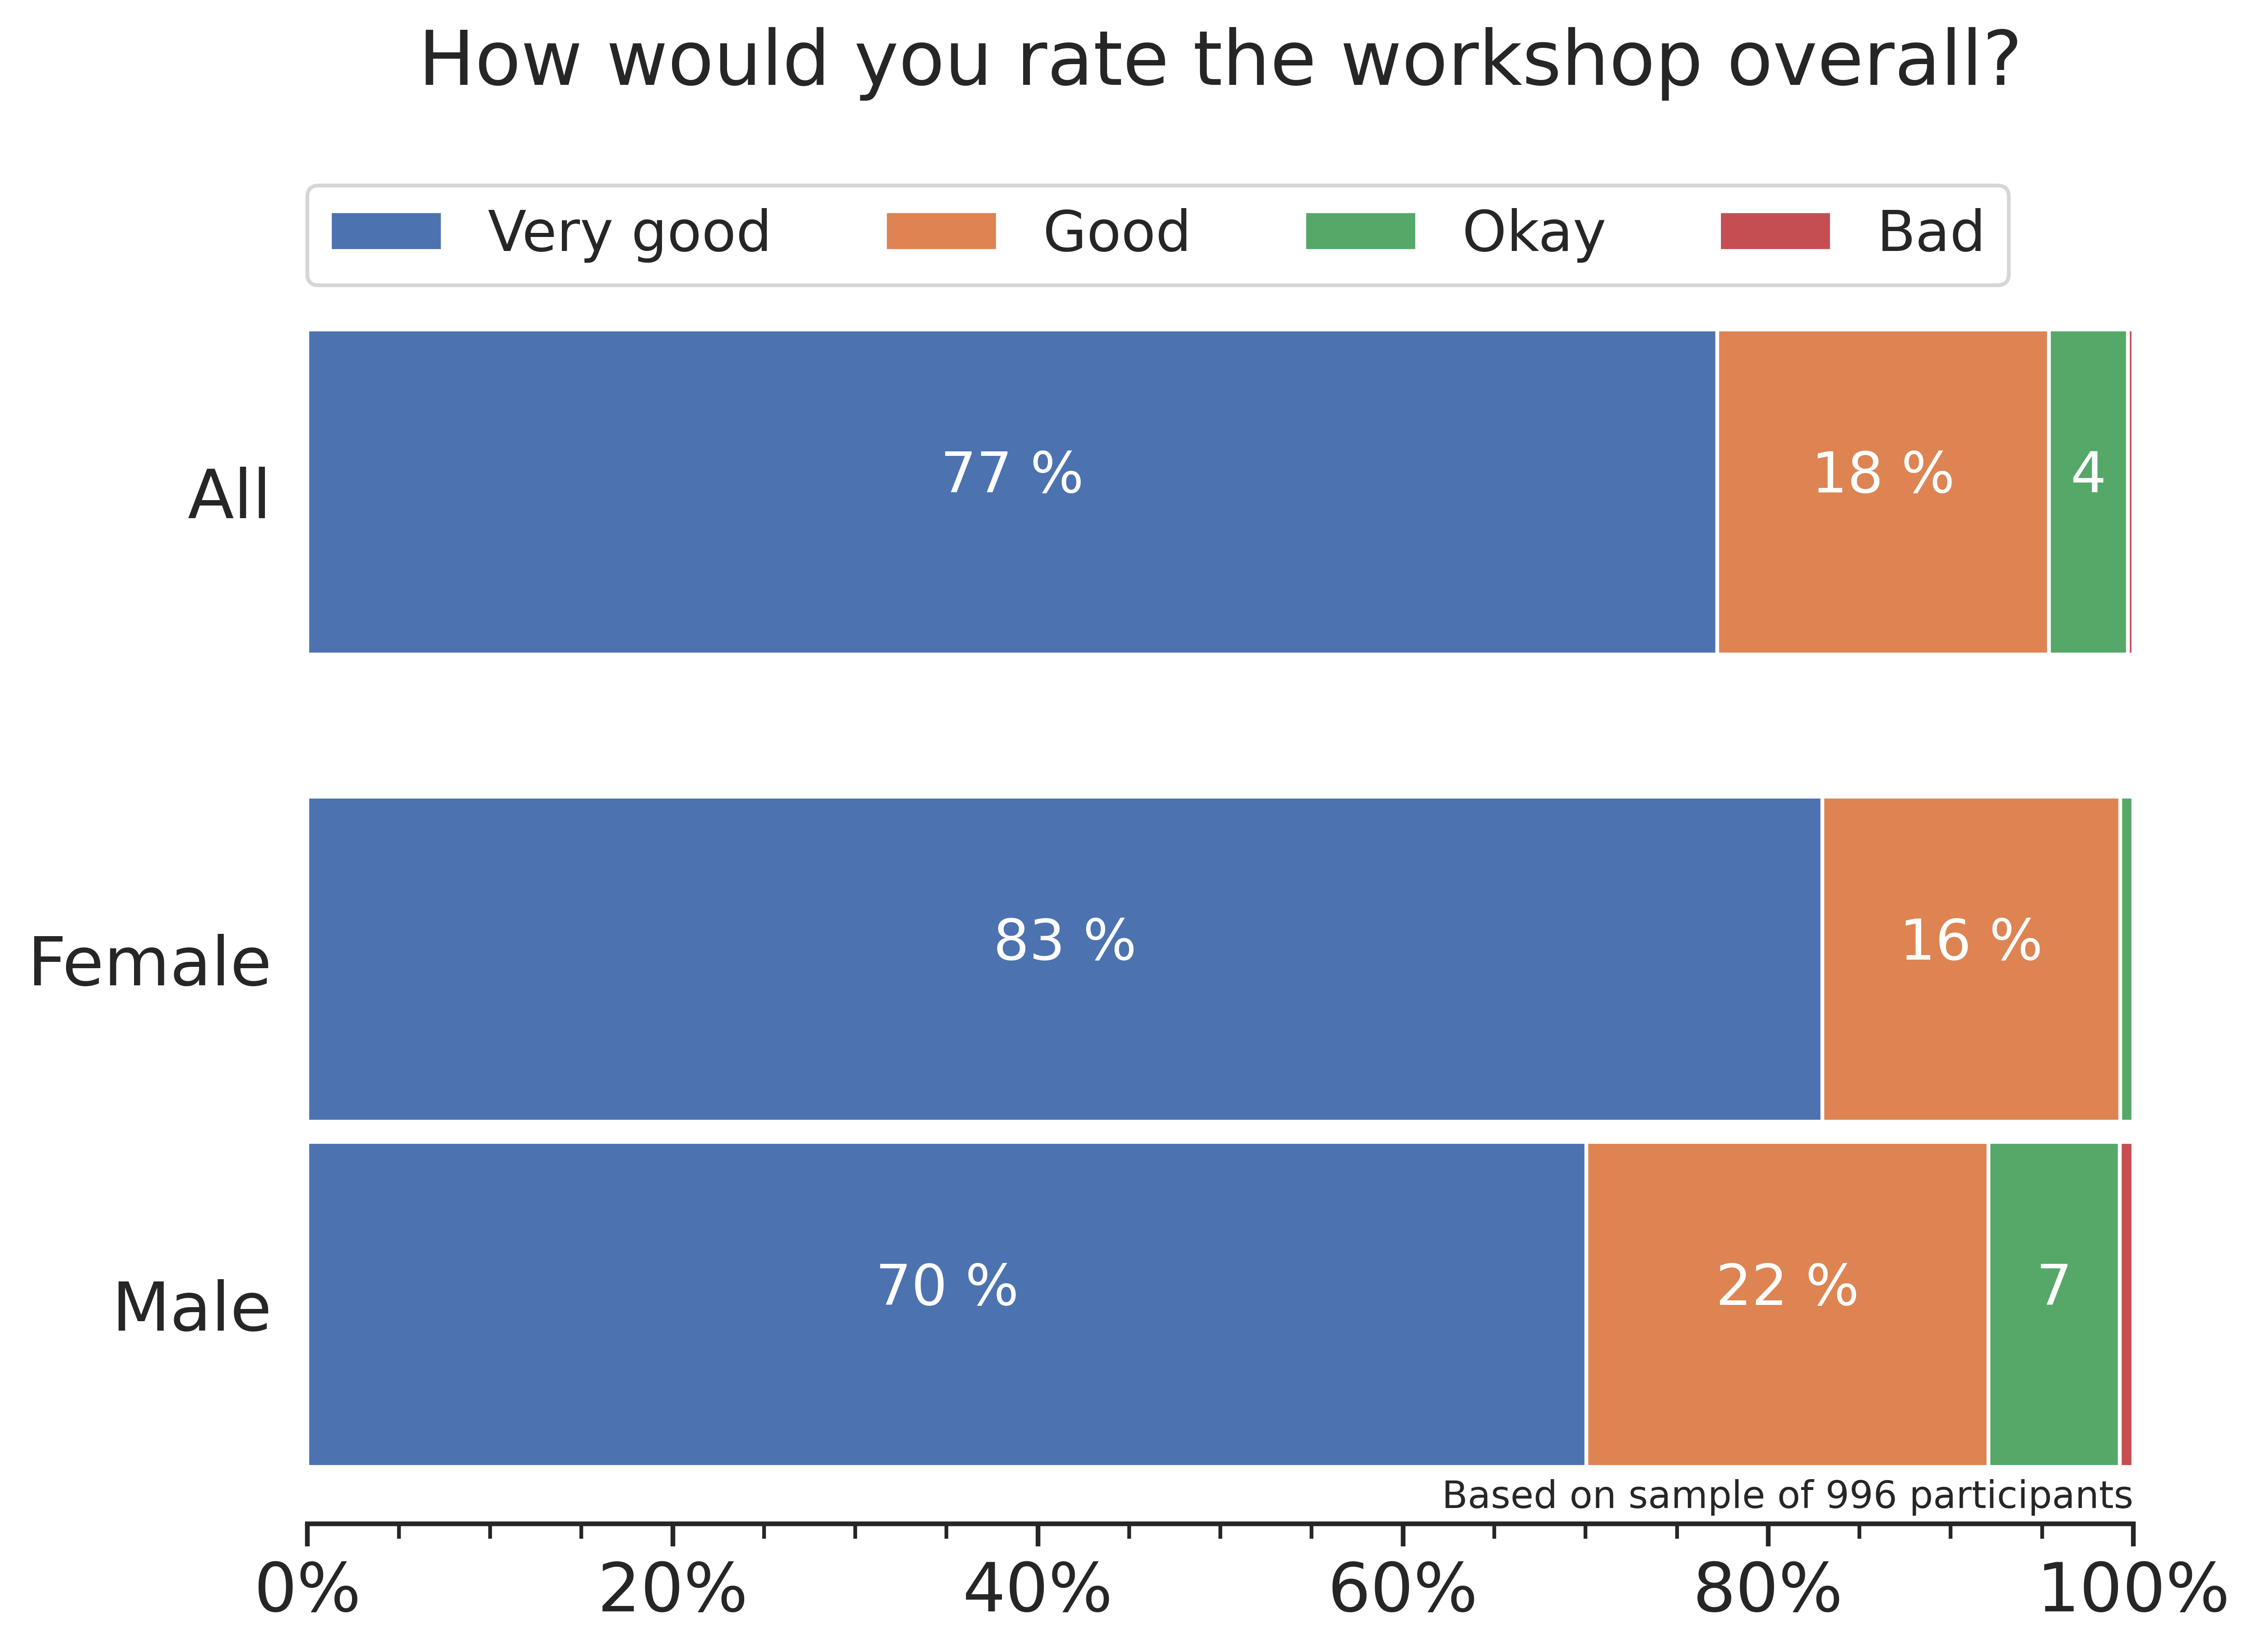
\includegraphics[width=0.85\textwidth]{bar_WorkshopFeedback}
    \caption{The participants were asked to rate their overall experience of the workshop. 77 per cent said it was very good, 18 per cent said good, four per cent said okay and less than one per cent said it was bad. Girls tend to report a more favourable opinion than boys.}
    \label{fig:ACworkshopexp}
\end{figure*}


\begin{figure*}[t!]
    \centering
        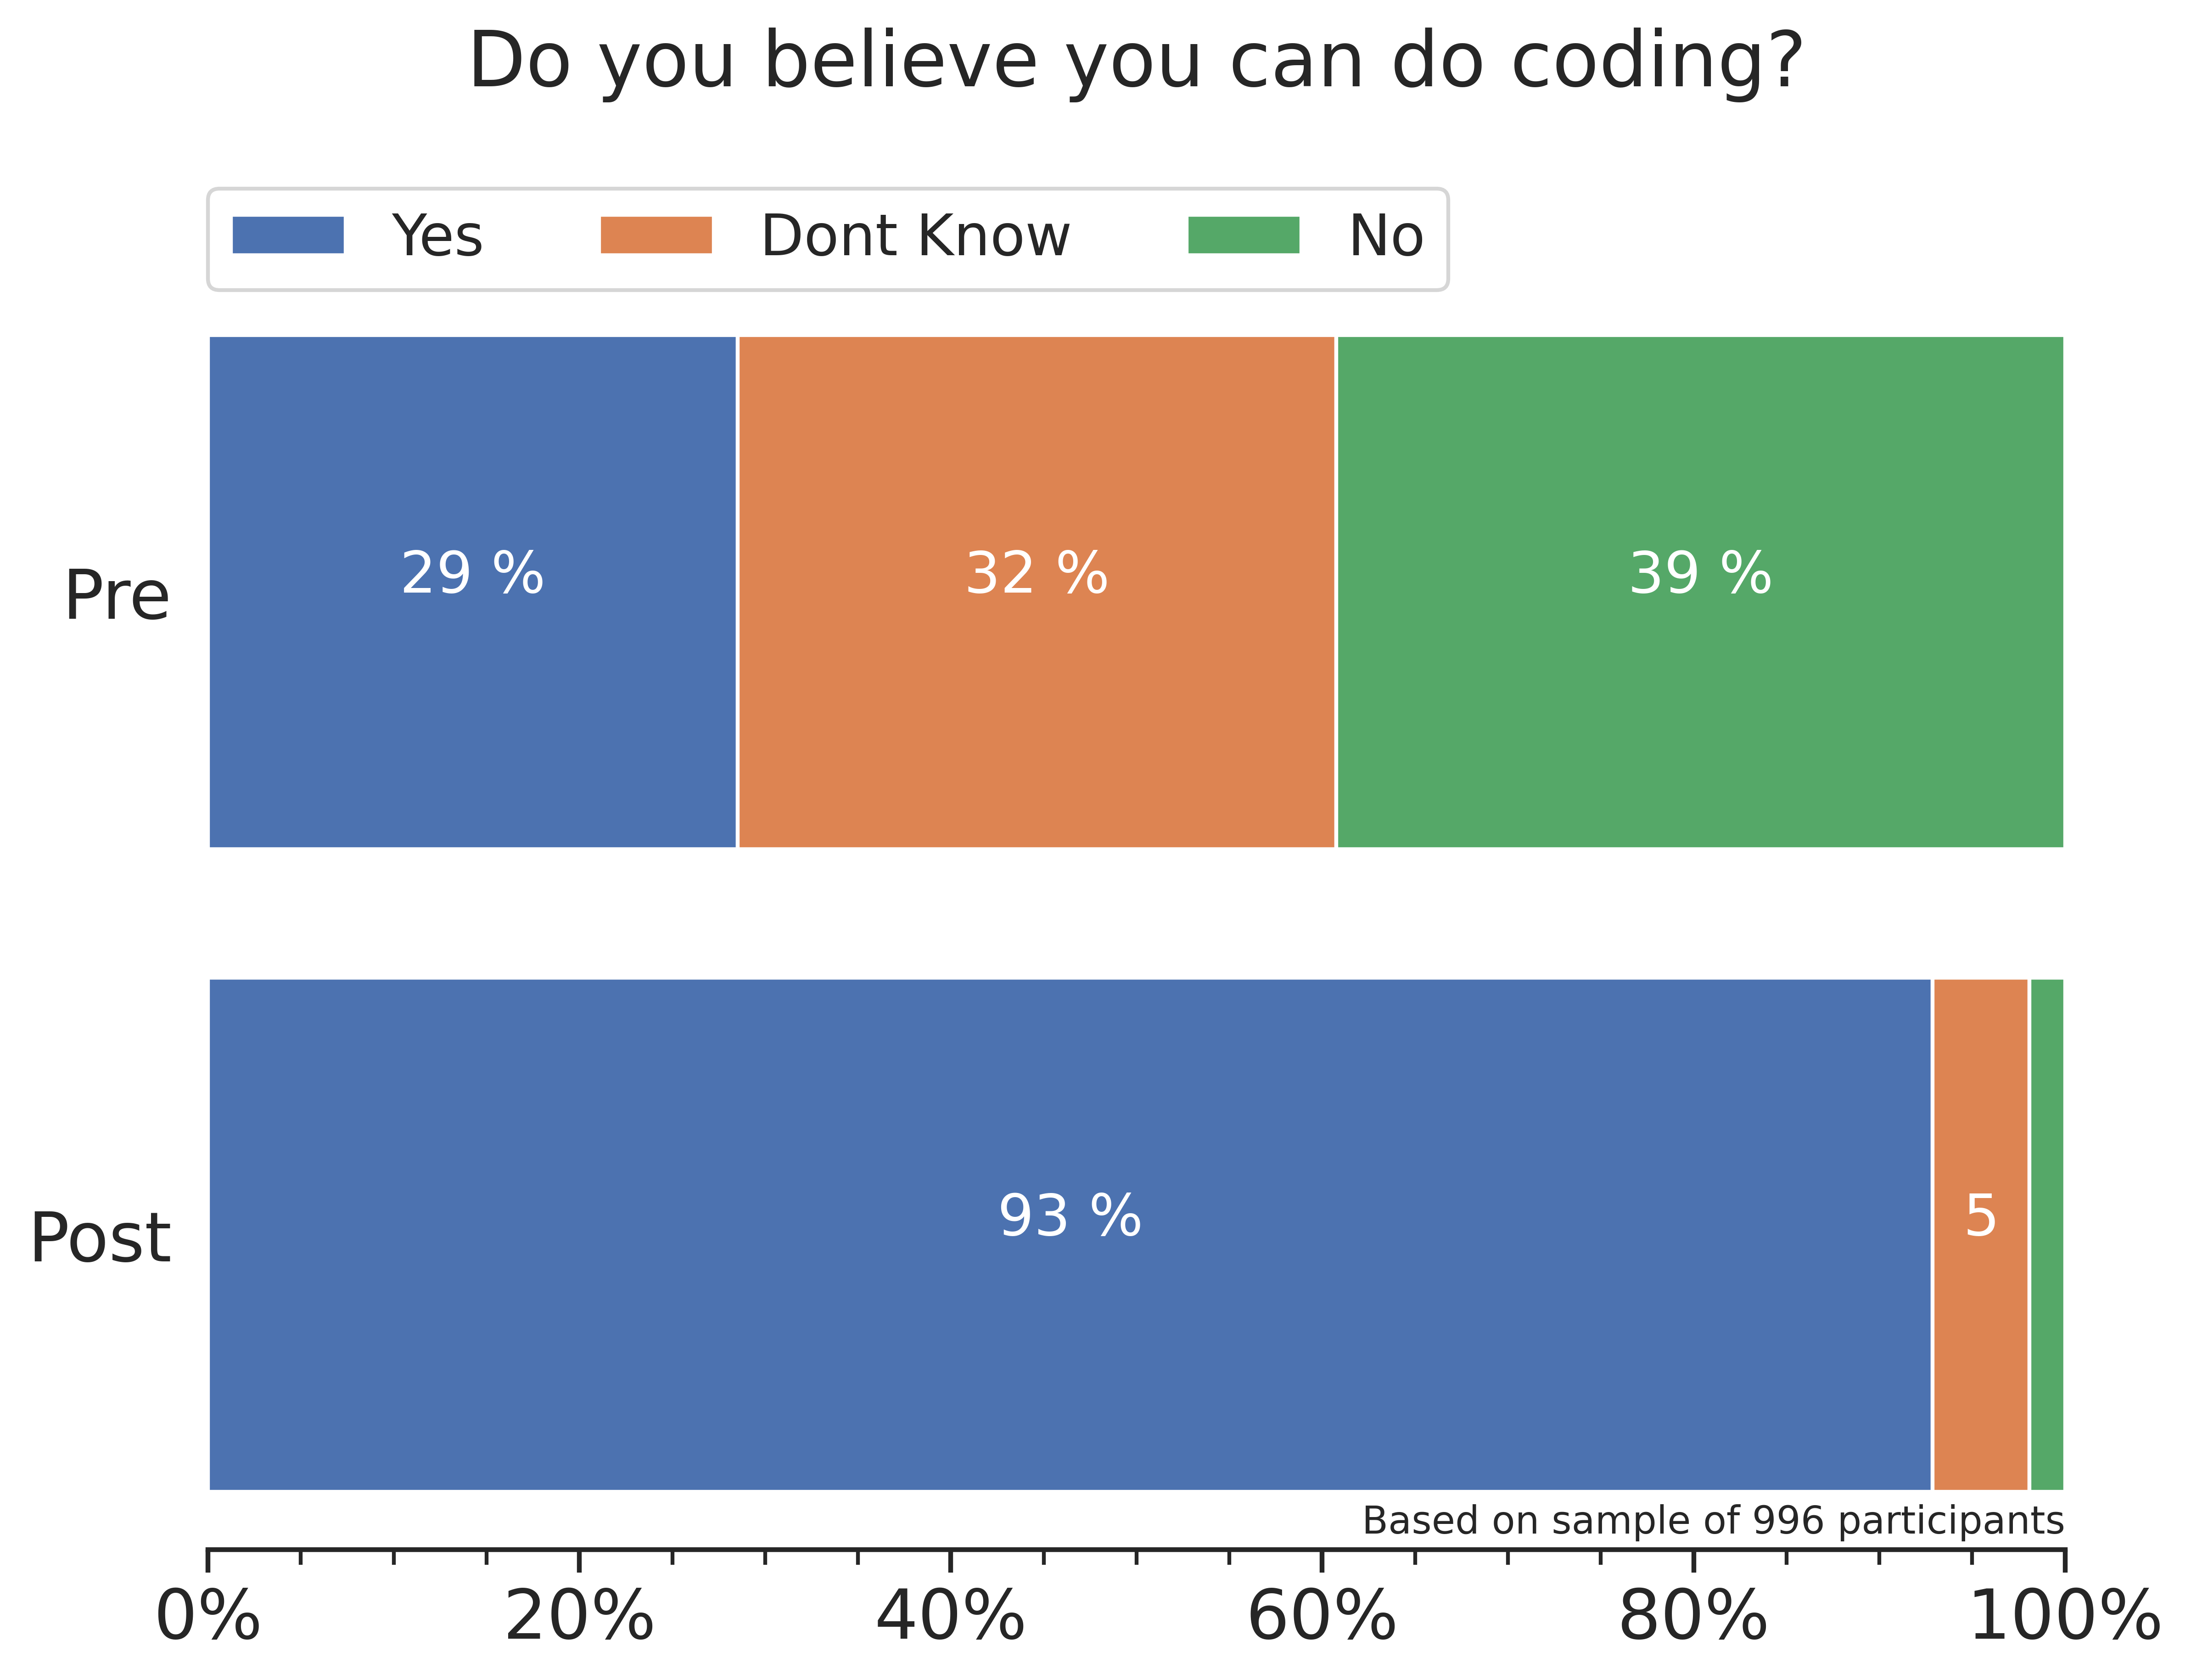
\includegraphics[width=0.85\textwidth]{bar_CanDoCoding}
\caption{The participants were asked before and after the workshop whether they believed they could do coding. There is a clear increase in confidence for the participants and their perceived ability to do coding. Prior to the workshop only 29 per cent felt they were able to do coding, 39 per cent of participants answered that were unable to do coding and 32 per cent didn't know whether they could. Following the workshop, 74 per cent felt they were able to do coding, with 14 per cent unsure and 12 per cent still not confident in their ability.} 
\label{fig:ACcandocoding}
\end{figure*}


\begin{figure*}[t!]
    \centering
        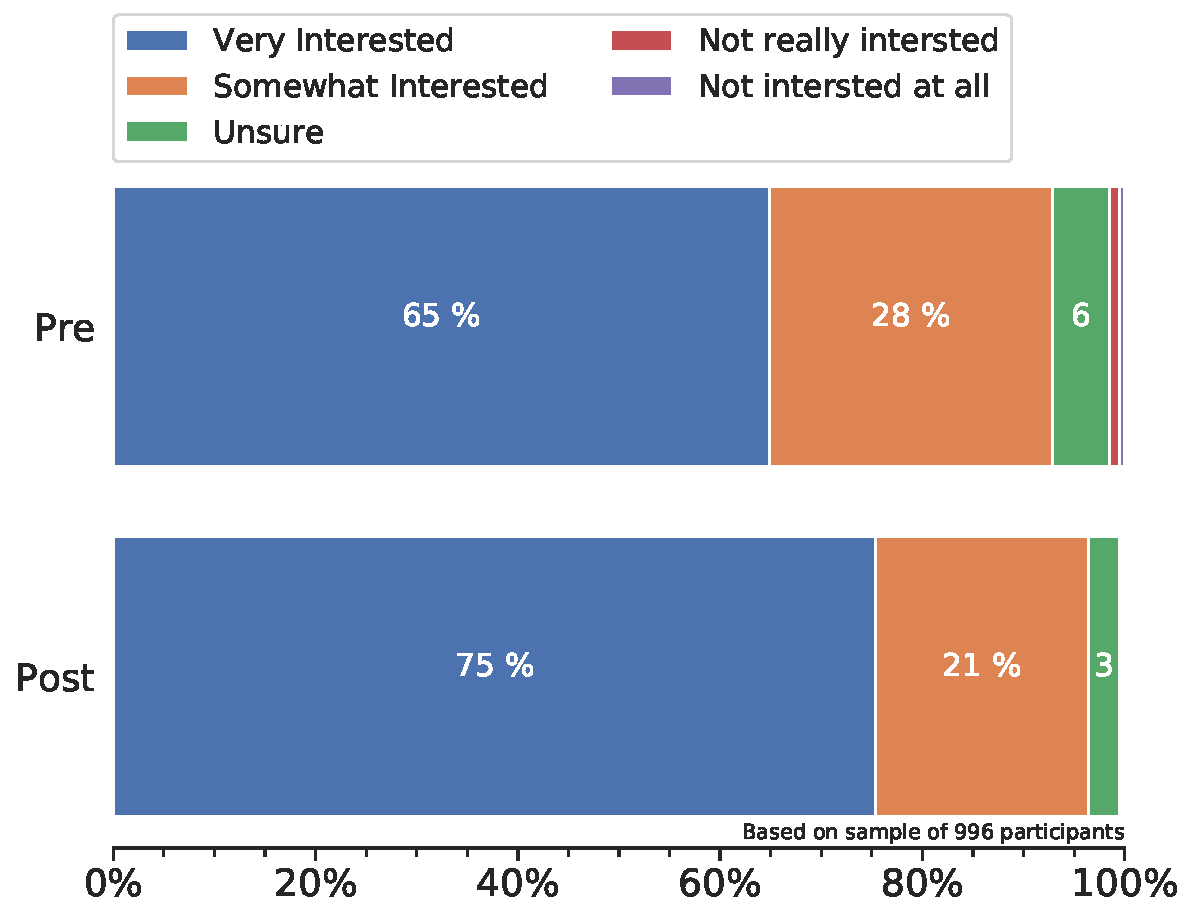
\includegraphics[width=0.85\textwidth]{bar_CodingInterest}
\caption{The participants were asked before and after the workshop how interested they are in doing coding. Despite an initially high interest, the workshops increase their interest in coding. The proportion of participants who are very interested in doing coding increased from 65 per cent before the workshop to 69 per cent after. And the proportion of participants who were not interested in learning coding or were unsure decreased from seven to four per cent.}
\label{fig:ACcodinginterest}
\end{figure*}


\begin{figure*}[t!]
    \centering
        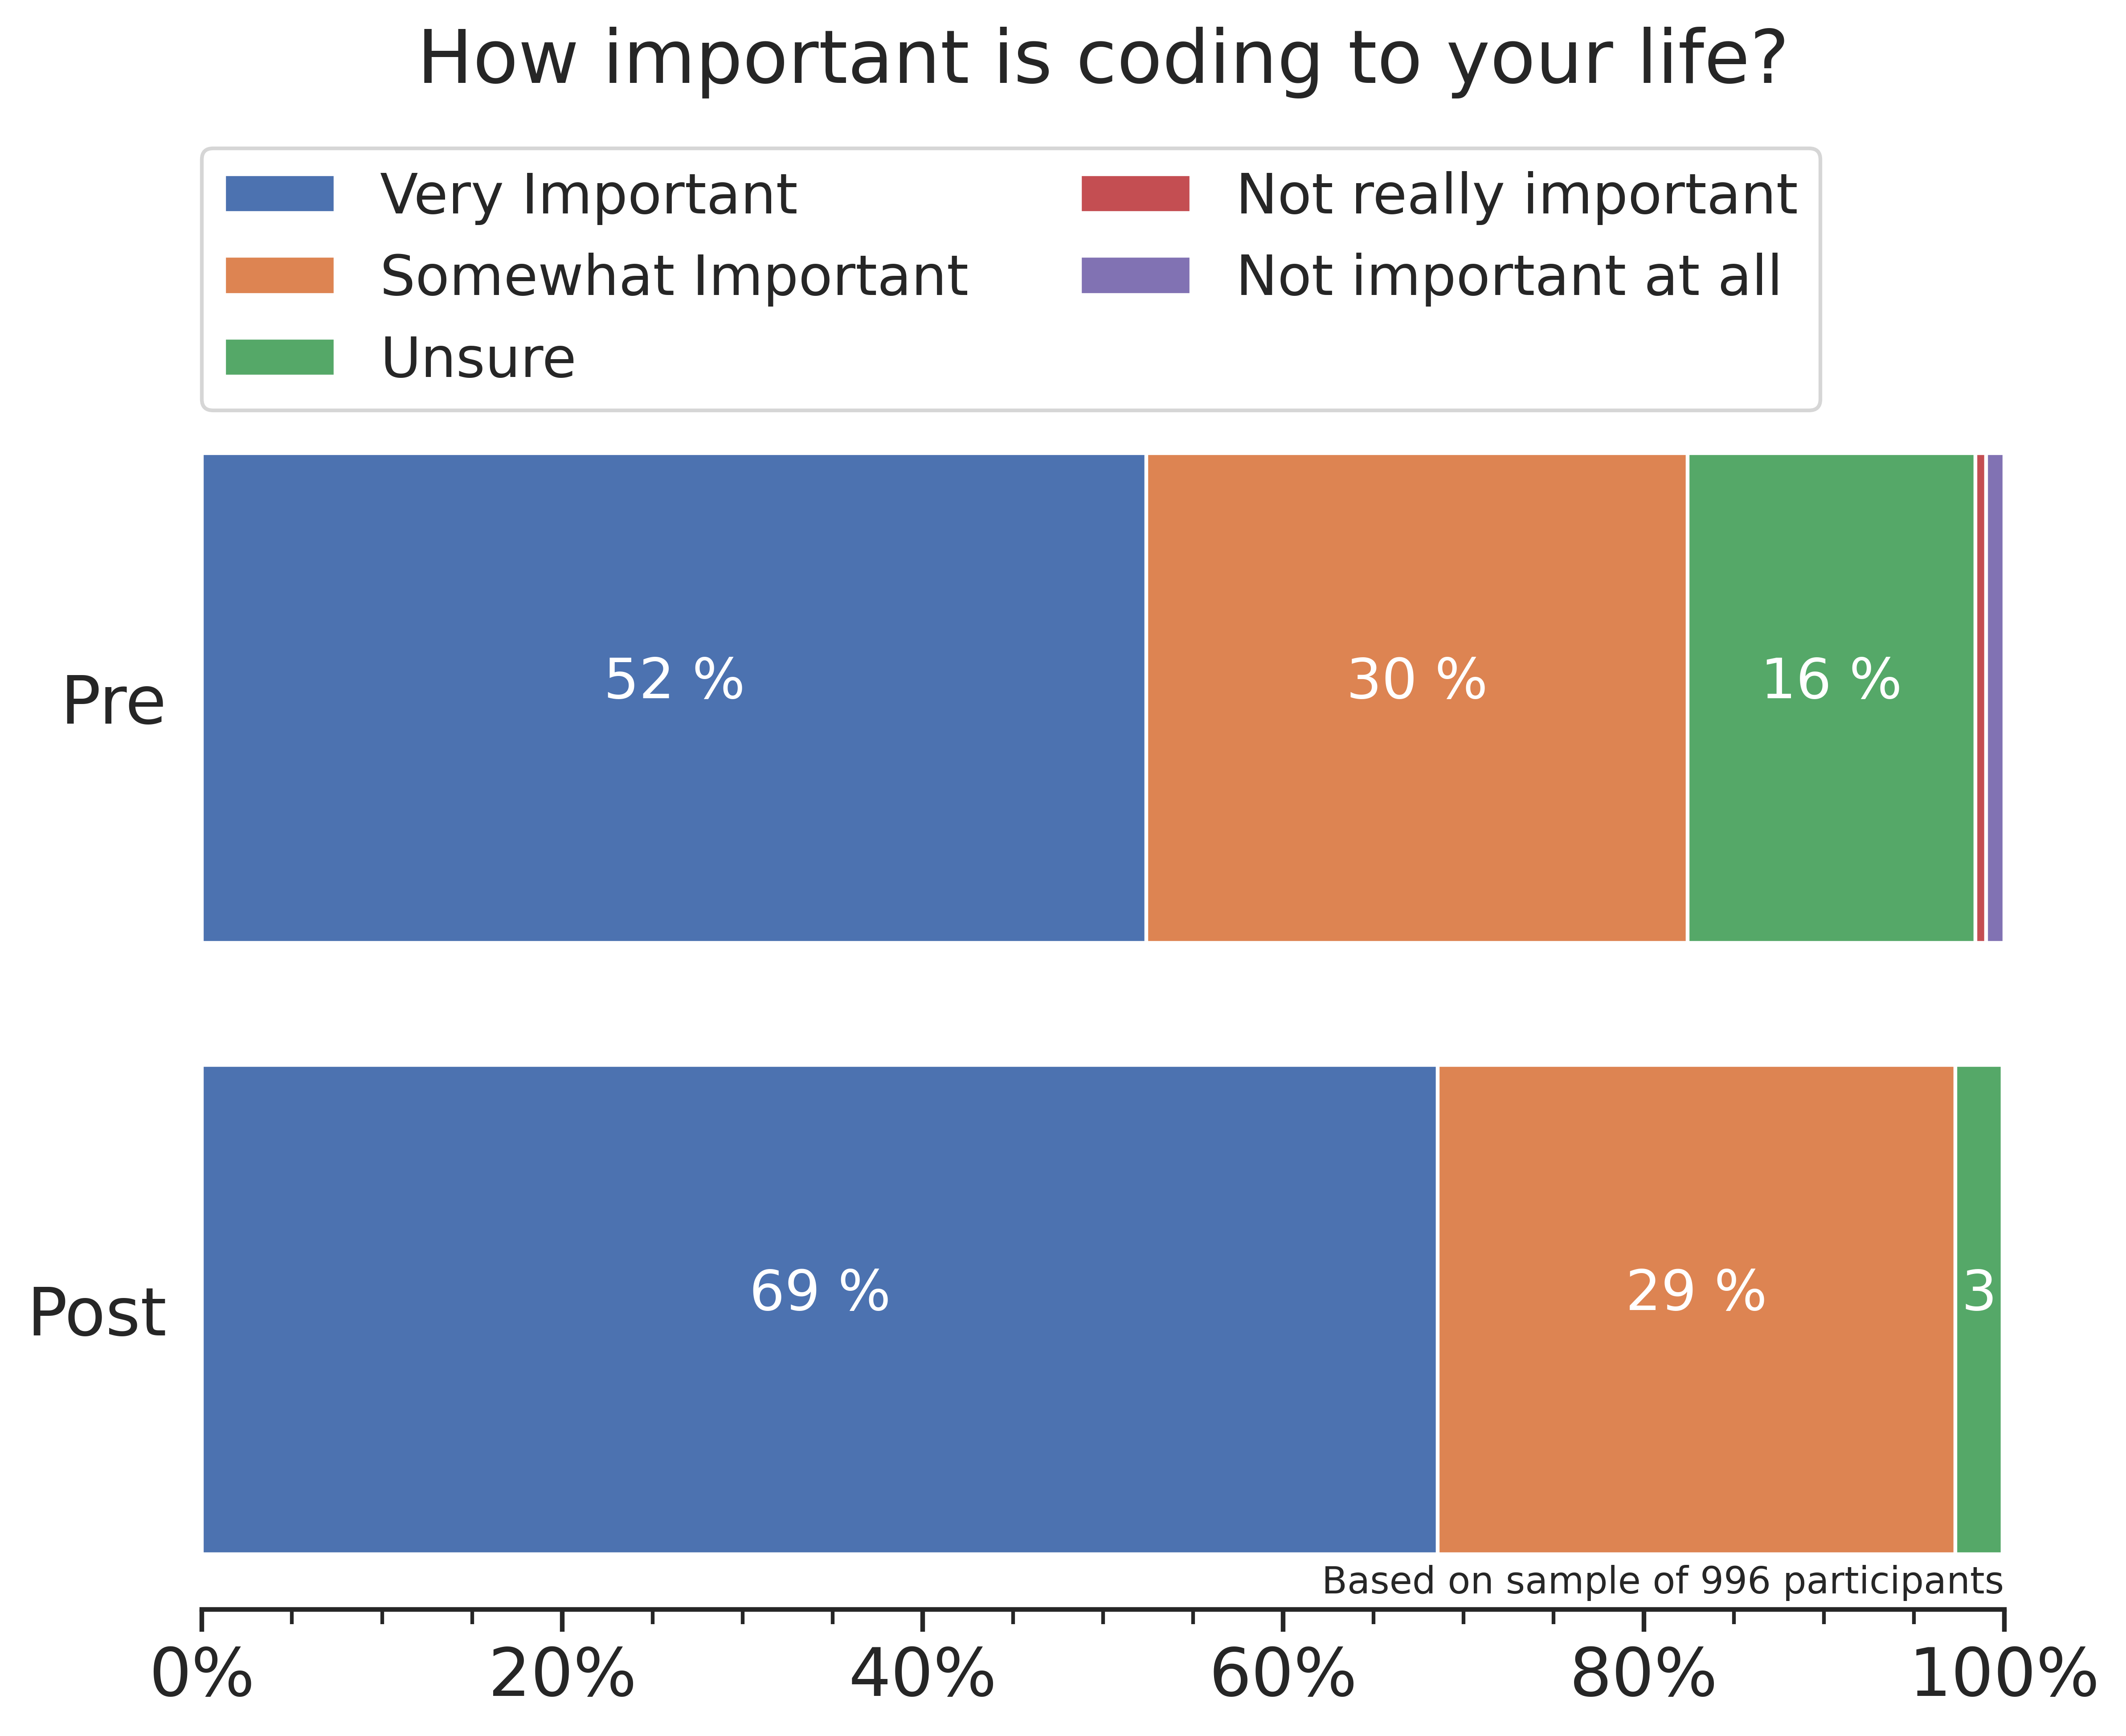
\includegraphics[width=0.85\textwidth]{bar_CodingImportance}
\caption{The participants were asked before and after the workshop how important they felt coding is to their lives. The workshops increased the perception of the participants in how important coding is to their lives. Prior to the workshop 18 per cent of participants felt coding was unimportant to their lives, or were unsure. After the workshop this reduced to only three per cent. The number who answered that coding was very important increased from 52 per cent to 69 per cent.}
\label{fig:ACcodingimportance}
\end{figure*}

\begin{figure*}[t!]
    \centering
        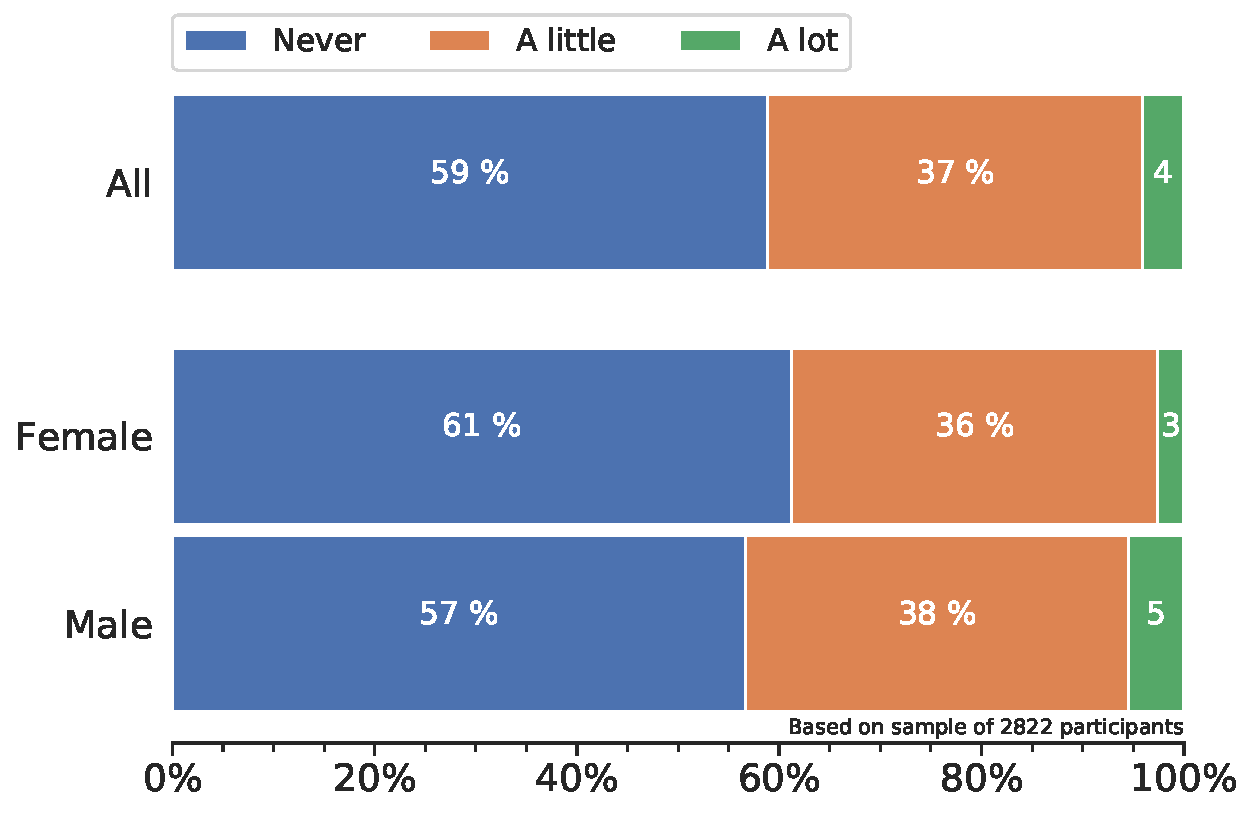
\includegraphics[width=0.75\textwidth]{bar_codedbefore}
\caption{The participants were asked whether they had done any coding before the workshop. The majority have not (59 per cent), with 37 per cent having done a little and only 4 per cent having done a lot. This question has been retired. }
\label{fig:codedbefor}
\end{figure*}

\begin{figure*}[t!]
    \centering
        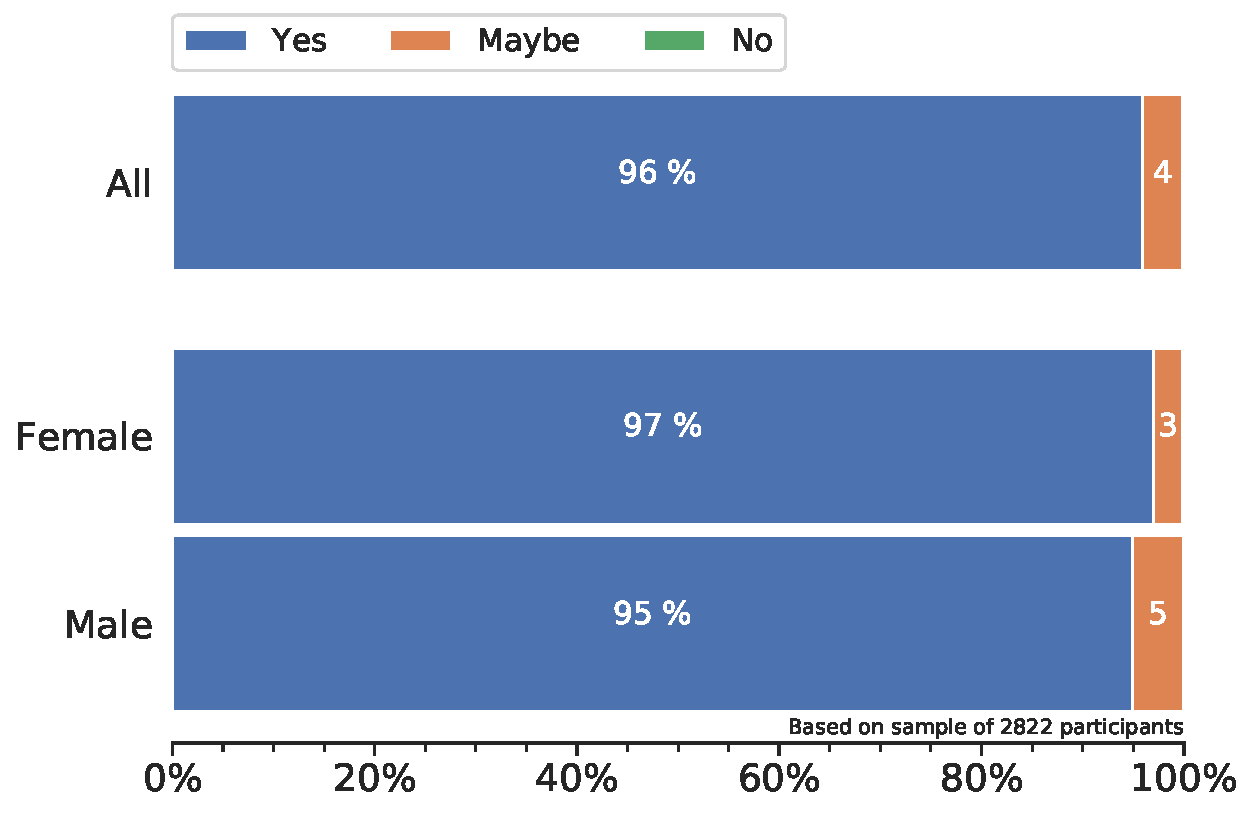
\includegraphics[width=0.75\textwidth]{bar_learnmore}
\caption{The participants were asked whether they would be interested in learning more coding after the workshop. Clearly the vast majority were interested. However this question was revised to include a pre-workshop measure of interest to determine the extent to which interest can be attributed to the workshop. This question has been retired.} 
\label{fig:learnmore}
\end{figure*}

\begin{figure*}[t!]
    \centering
        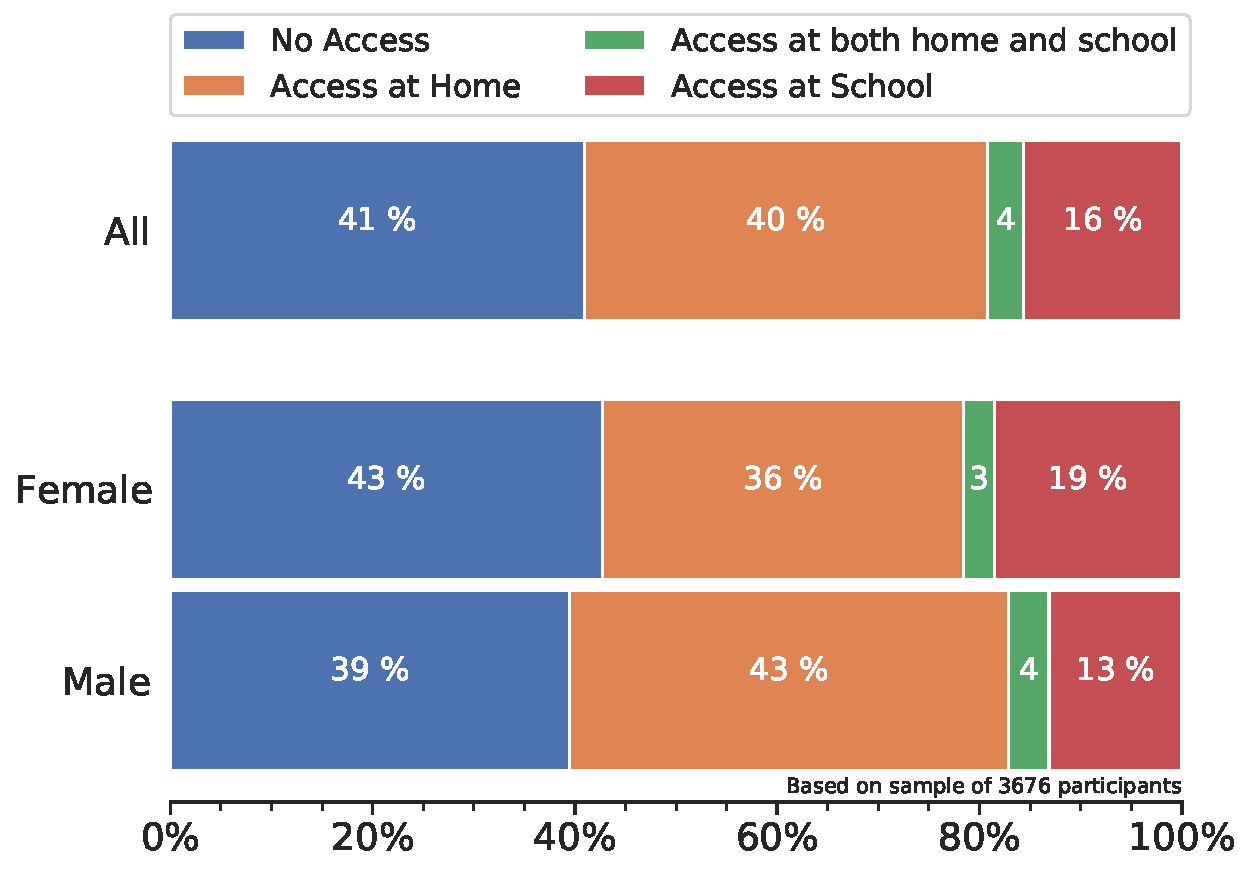
\includegraphics[width=1\textwidth]{bar_ITaccess}
\caption{The participants were asked whether they have regular access to a computer at home or at school. 41 per cent of participants said they do not have regular access to a computer at home or at school, highlighting the important role libraries can play in providing access. Another 40 per cent have access at home and 20 per cent have access at school. } 
\label{fig:itaccess}
\end{figure*}

\begin{figure*}[t!]
    \centering
        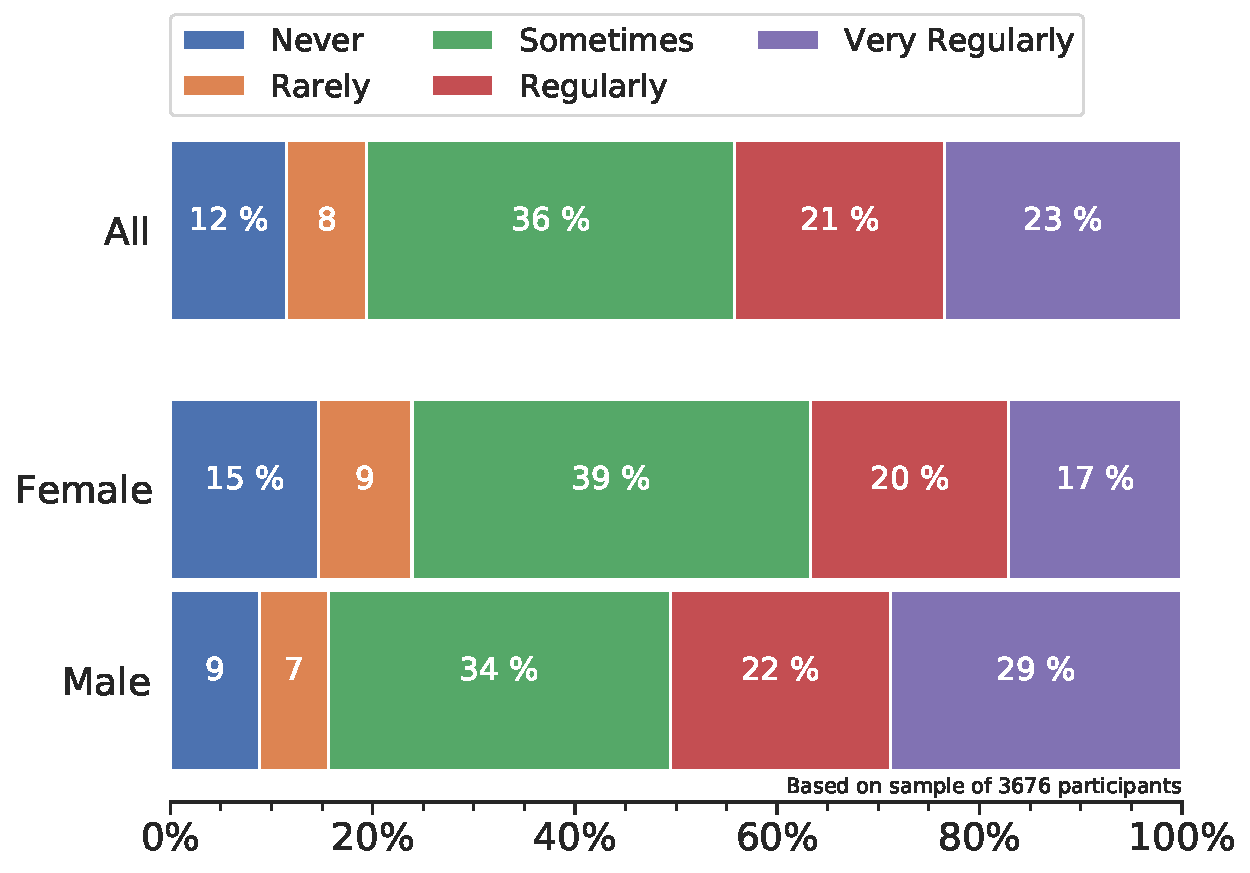
\includegraphics[width=1\textwidth]{bar_UseComputersOften}
\caption{The participants were asked how often they use a computer. The following definitions were used:  \textit{``Never''} = first time using a computer,  \textit{``Rarely''} = once or twice a year, \textit{``Sometimes''} = once per month,  \textit{``Regularly''} = at least once a week and  \textit{``Very regularly''} = many times a week. We find that 12 per cent had never used a computer prior to the workshop (this is higher in girls with proportion of 15 per cent compared to 9 per cent of boys). We also find that boys are much more likely to report to using computers very regularly with 30 per cent of boys doing so compared to only 17 per cent of girls. } 
\label{fig:itusefreq}
\end{figure*}


\begin{figure*}[t!]
    \centering
        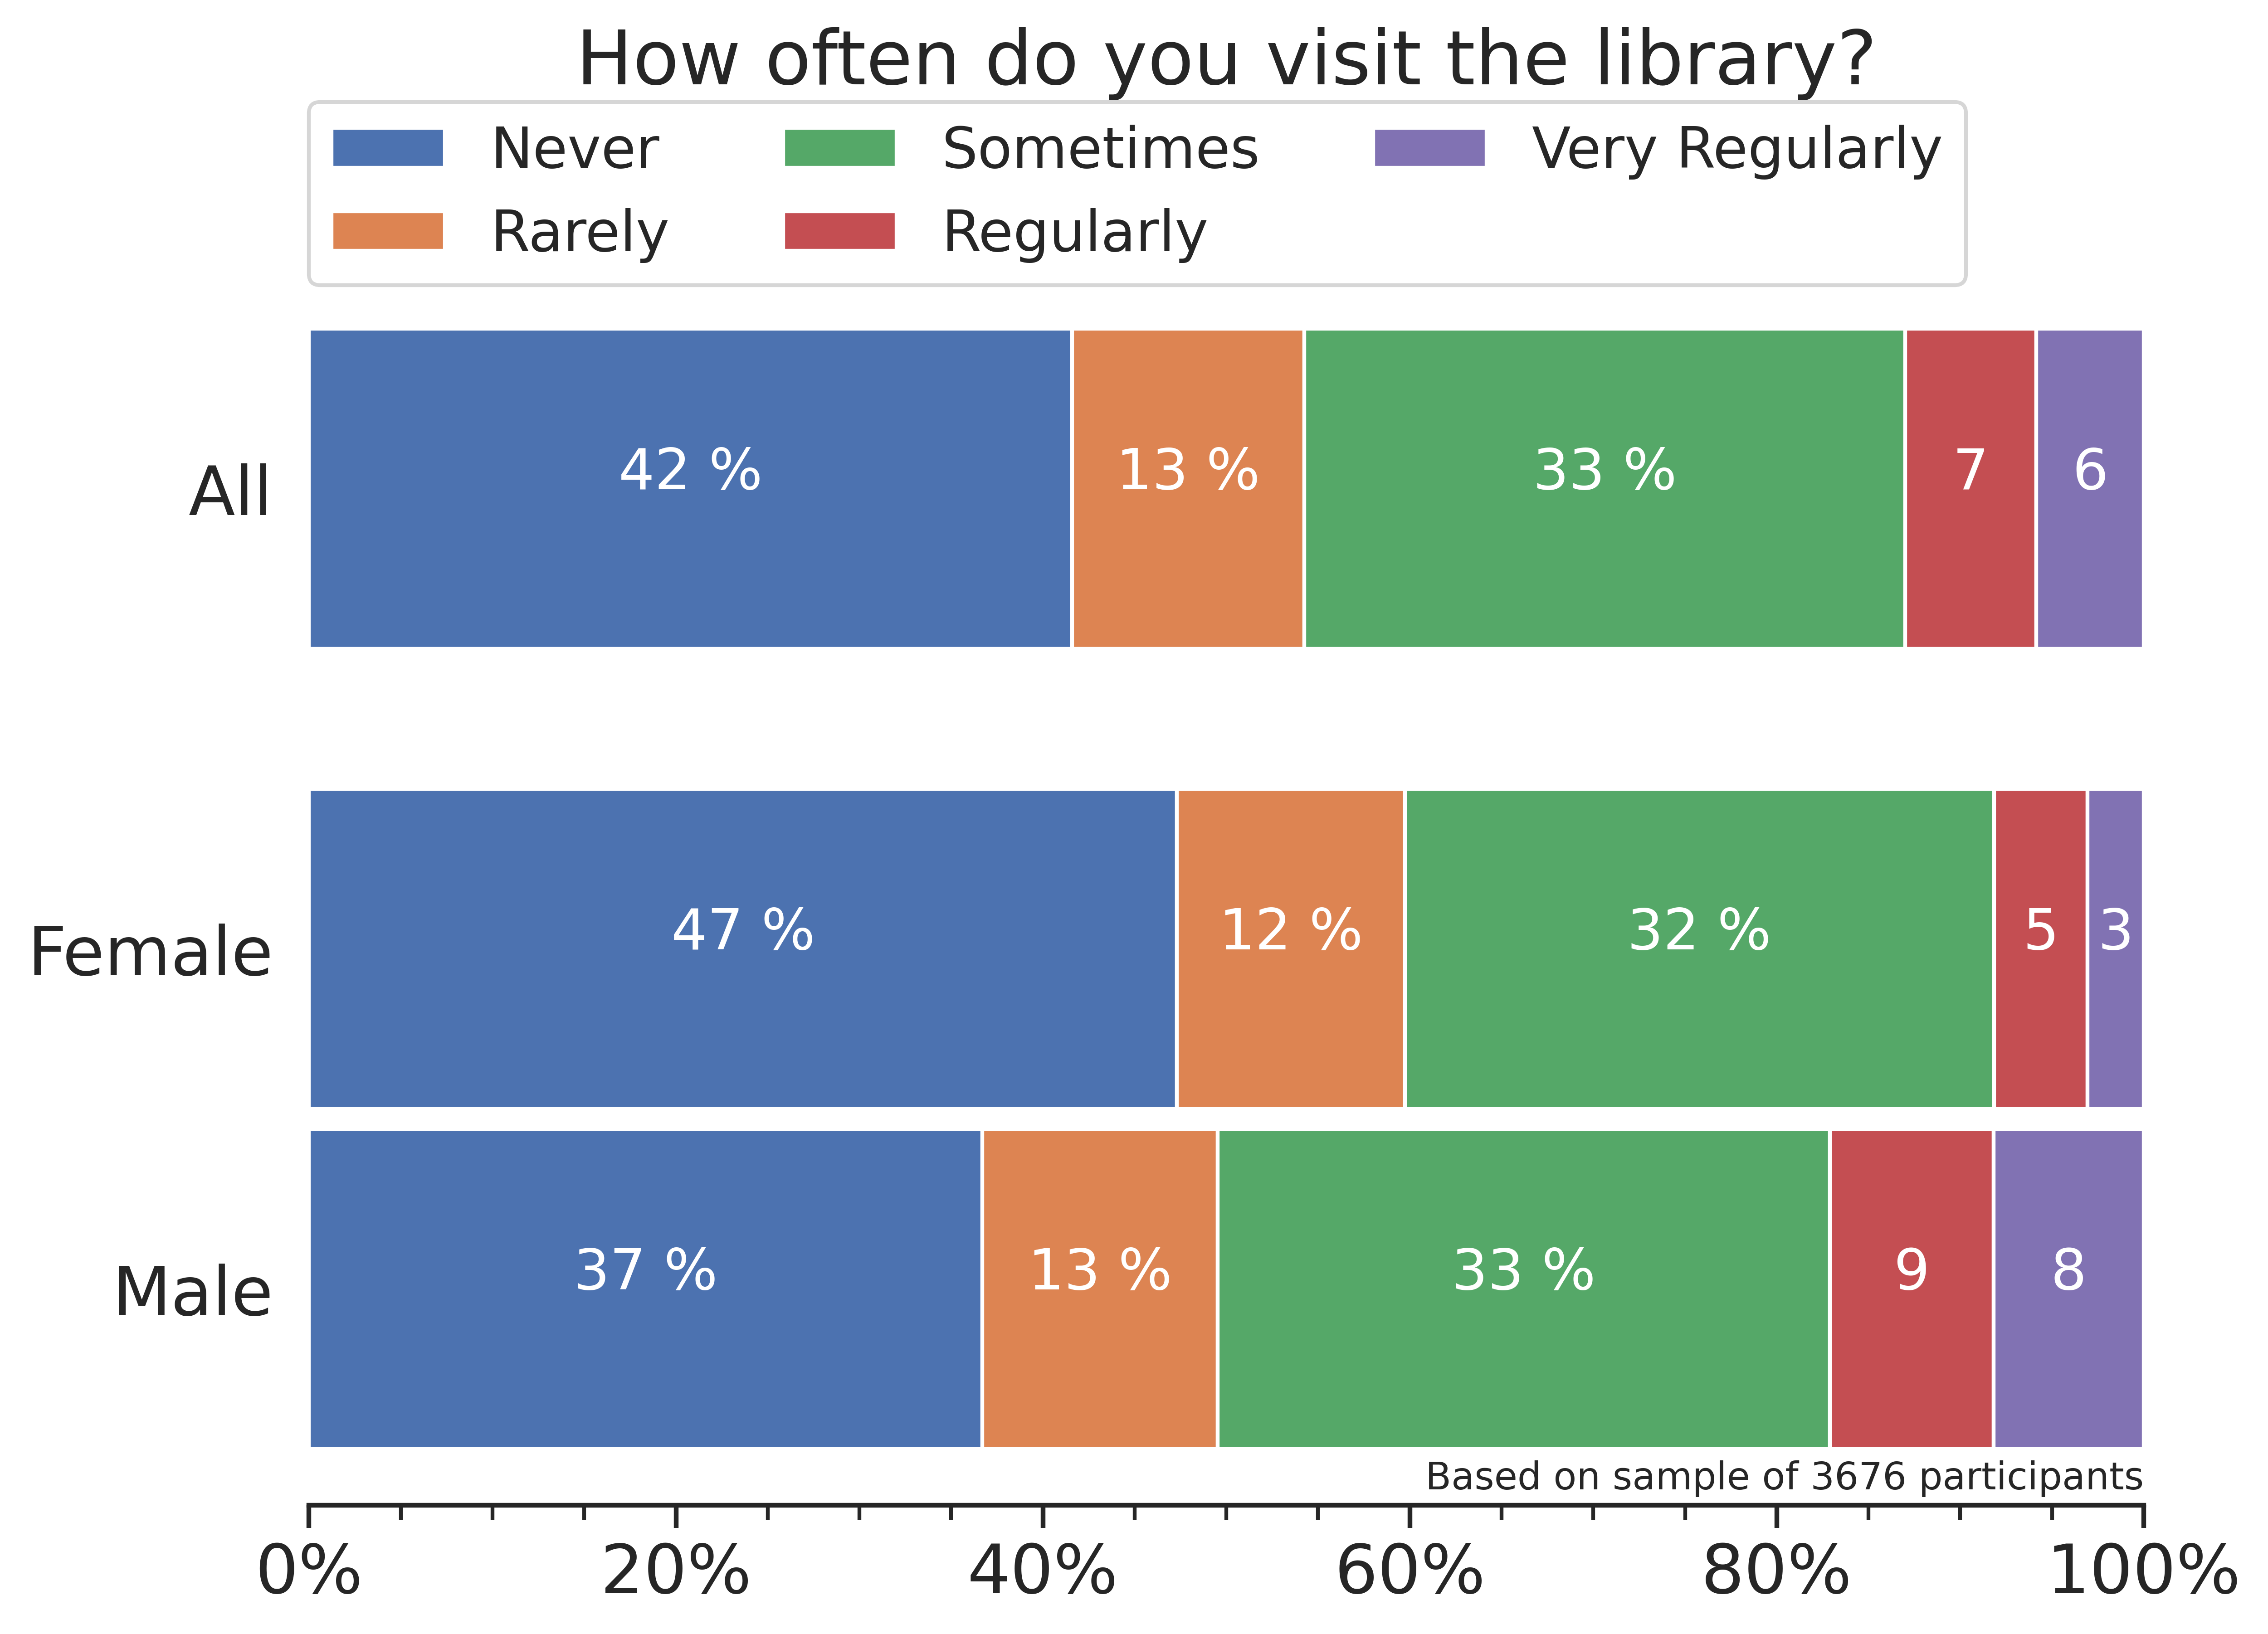
\includegraphics[width=1\textwidth]{bar_VisitLibraryBefore}
\caption{The participants were asked how often they use a library (not including their school library). The following definitions were used:  \textit{``Never''} = first time in a library,  \textit{``Rarely''} = once or twice a year, \textit{``Sometimes''} = once per month,  \textit{``Regularly''} = at least once a week and  \textit{``Very regularly''} = many times a week. 42 per cent of participants had never used the library prior to our workshop, a proportion which is higher in the girls (48 per cent compared to 38 per cent of the boys). The workshops are introducing young people to their local library. Less than 50 per cent of participants report to be using the libraries on even a monthly basis (i.e. ''sometimes'', ''regularly'' and ''very regularly'' combined). And less than 13 per cent are using the libraries on a weekly or daily basis (i.e. ''regularly'' and ''very regularly'').} 
\label{fig:libusefreq}
\end{figure*}

\begin{figure*}[t!]
    \centering
        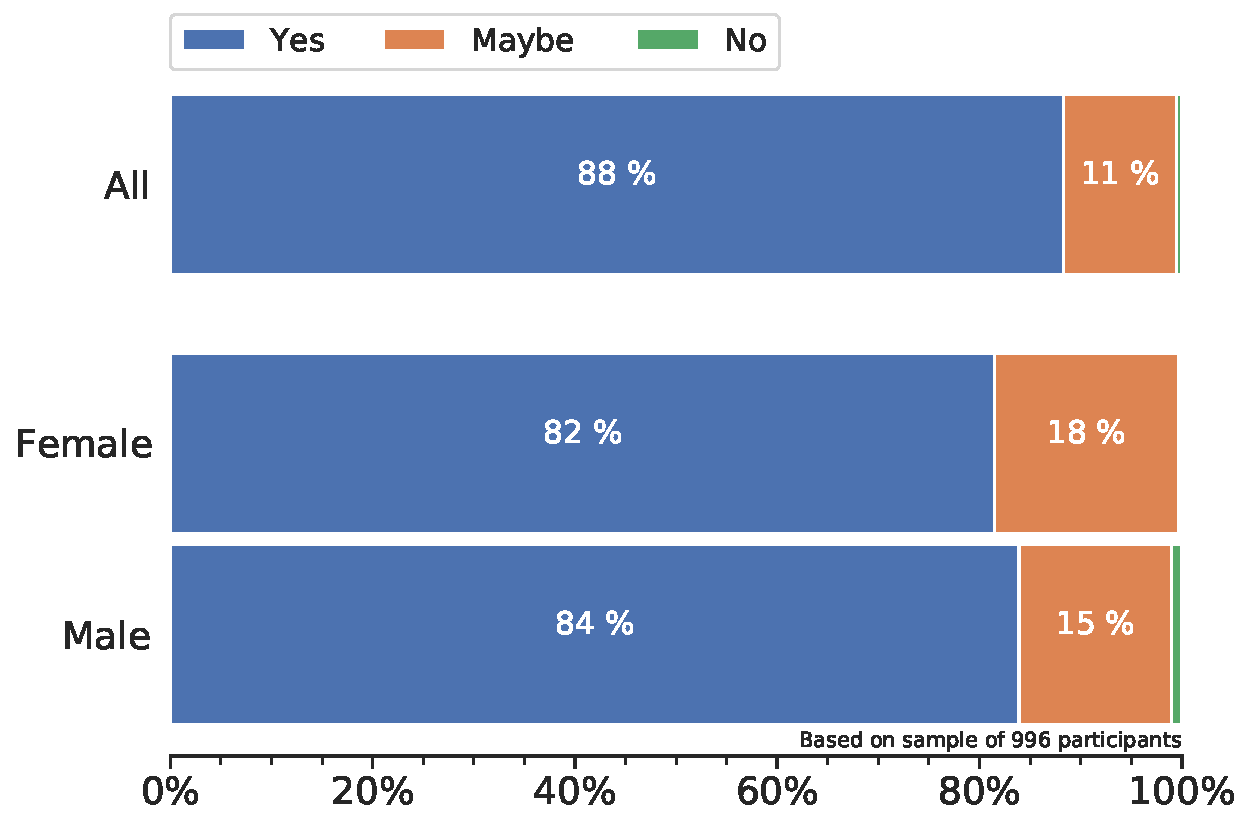
\includegraphics[width=1\textwidth]{bar_VisitLibrary_Activities}
\caption{The participants were asked whether they would visit the library more often if activities like this [the workshop] were offered. The positive response to this question, with 88 per cent saying yes, shows the potential for attracting new library users through the introduction of innovative new services.  } 
\label{fig:libraryvisitactivities}
\end{figure*}

\begin{figure*}[t!]
    \centering
        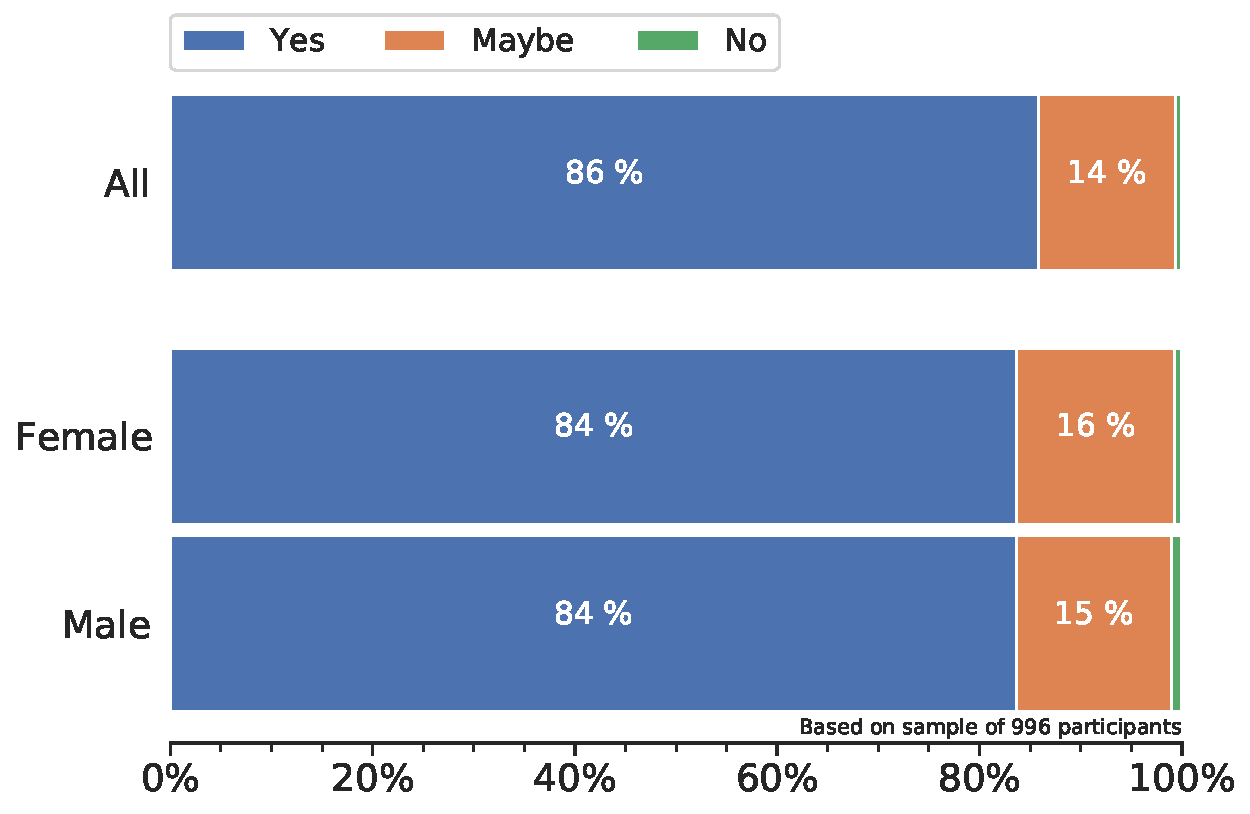
\includegraphics[width=1\textwidth]{bar_VisitLibrary_Devices}
\caption{The participants were asked whether they would visit the library regularly if the devices [micro:bit and Kano] are made publicly available. The vast majority answered positively (with $84$ per cent answering yes), highlighting the potential for attracting new library users through the introduction of innovative new services.} 
\label{fig:libraryvisitdevices}
\end{figure*}

\begin{figure*}[t!]
    \centering
        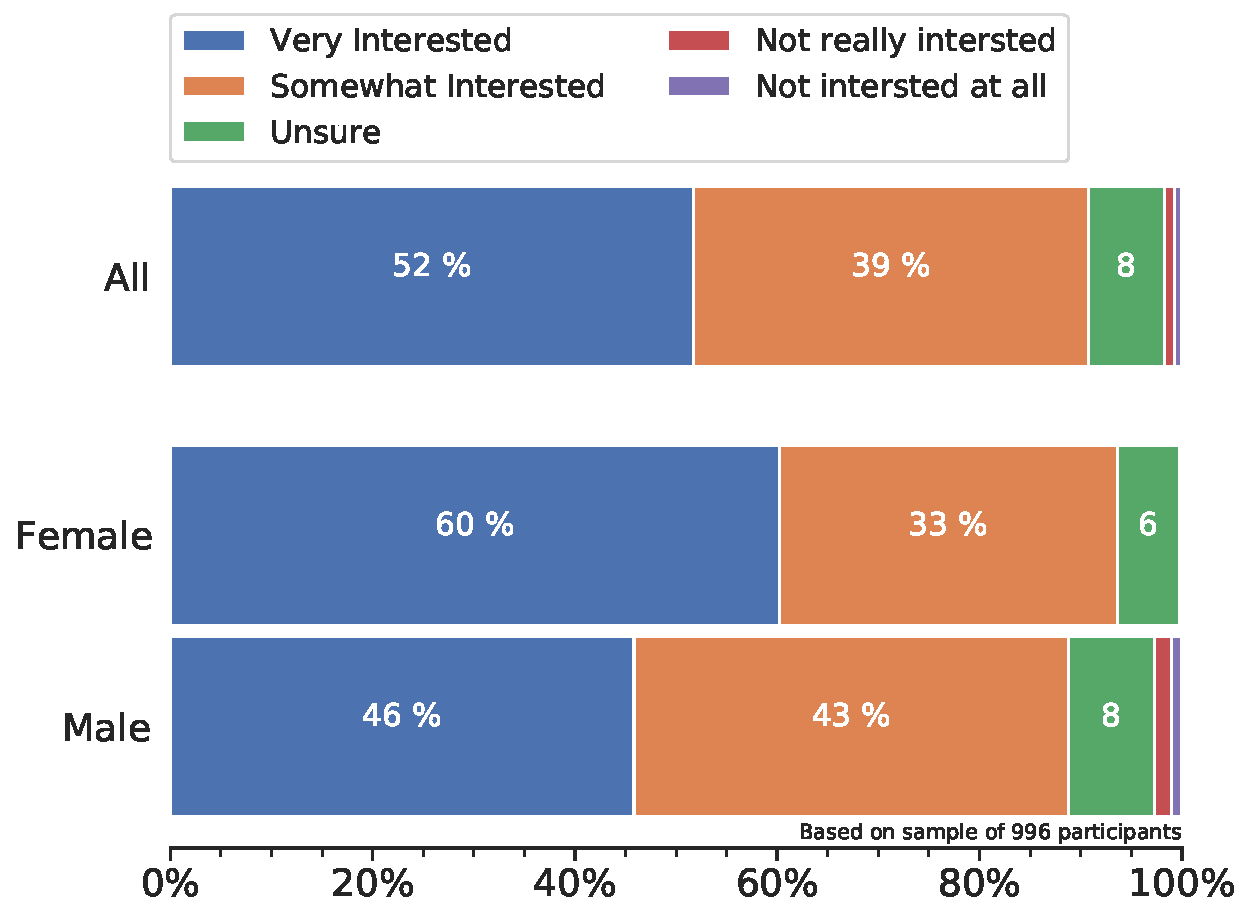
\includegraphics[width=1\textwidth]{bar_DesireLibraryVisit}
\caption{The participants were asked before the workshop how interested they are in visiting the library. The vast majority express an interest in using the library, with 52 per cent reporting to be ''very interested'' and a further 39 per cent ''interested''. }
\label{fig:libvisitinterest}
\end{figure*}


\begin{figure*}[t!]
    \centering
        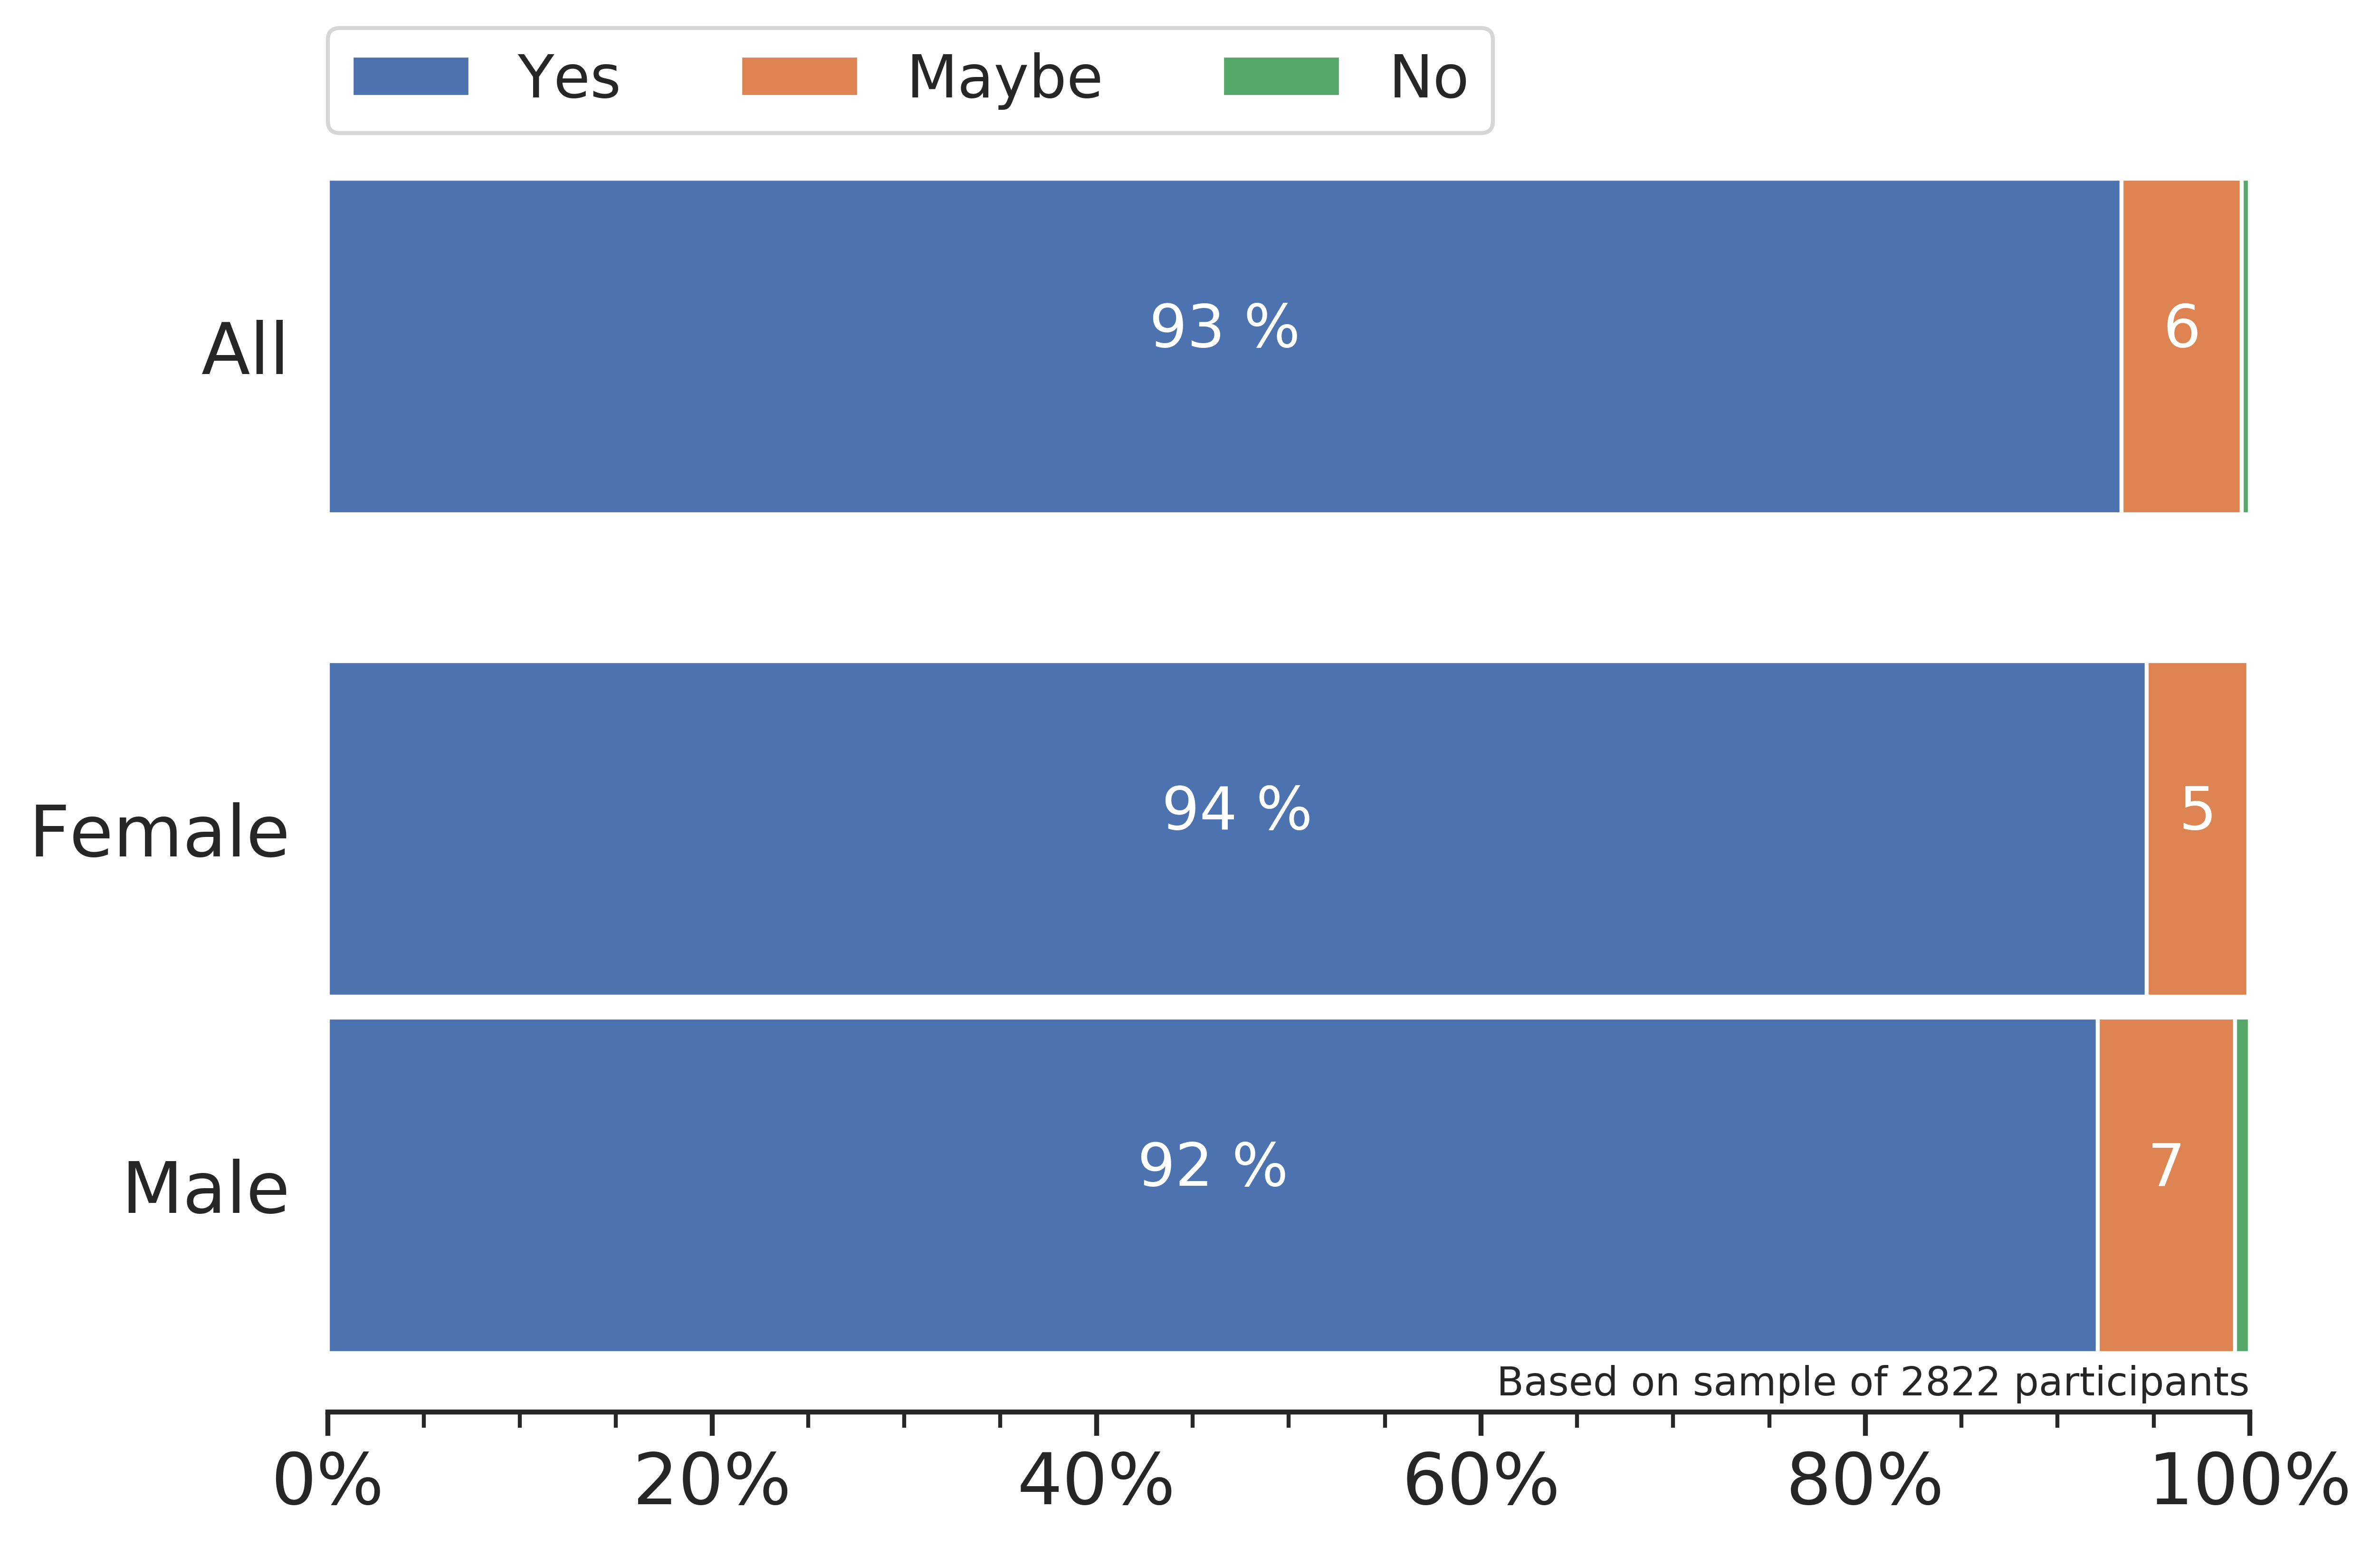
\includegraphics[width=1\textwidth]{bar_usedevices}
\caption{The participants were asked ``if the devices [micro:bit and Kano] were publicly available in the library would you use them?''. The vast majority answered positively (with $>95$ per cent answering yes). This question has been retired. } 
\label{fig:usedevices}
\end{figure*}



\begin{figure}[!htb]
\center{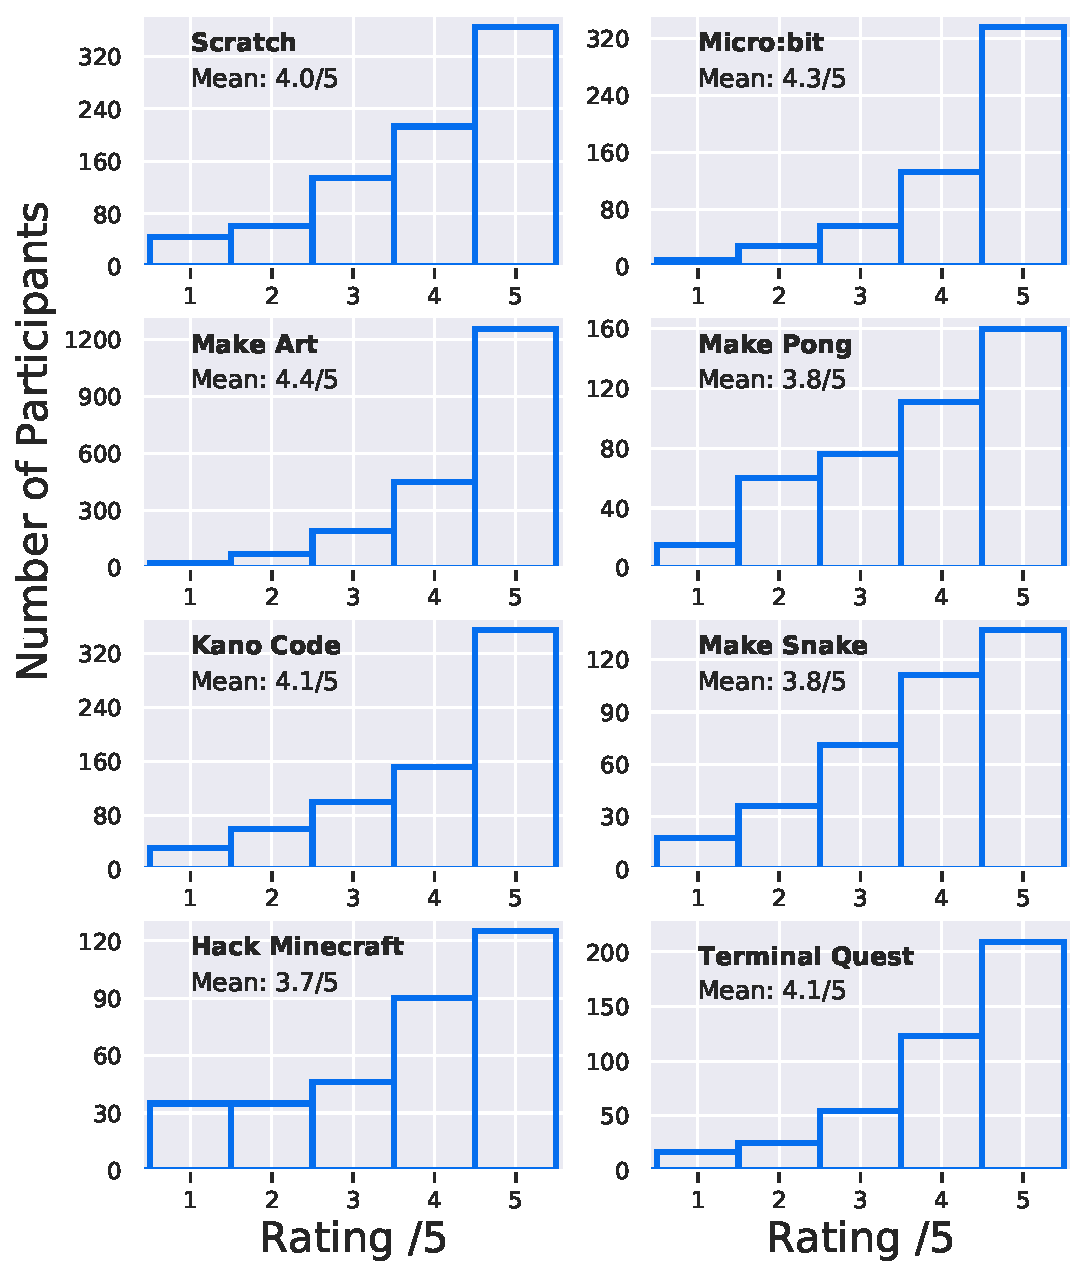
\includegraphics[width=0.9\linewidth]{AppRatings}}
\caption{The participants were asked which coding app or activity they participated in and to rate this out of five (where 0 is hated it and 5 is loved it). These histograms show the distribution of ratings for each app, as well as the mean rating for each app. This question is primarily for our internal understanding. Make Art and micro:bit have proven to be the most favored activities with the participants. } 
\label{fig:appratings}
\end{figure}

\begin{figure*}[t!]
    \centering
        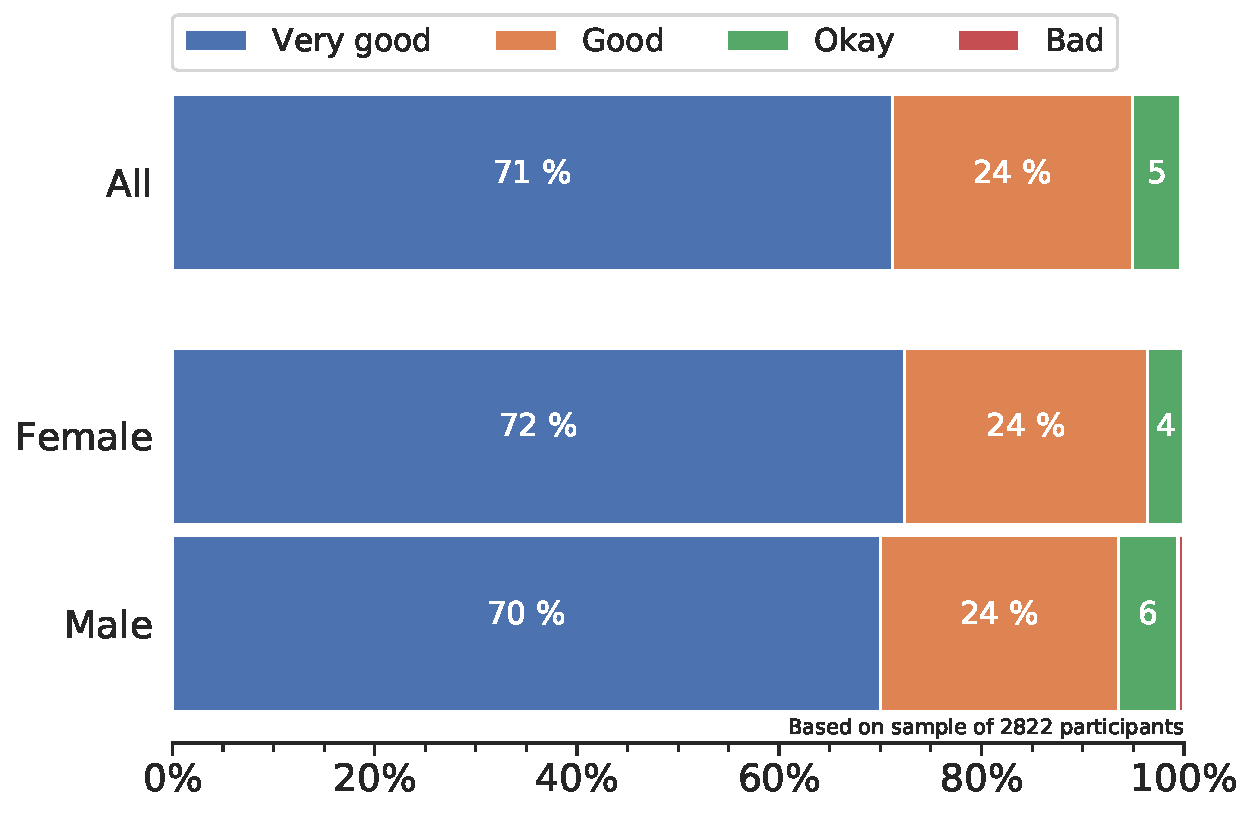
\includegraphics[width=0.7\textwidth]{bar_kanoexp}
    \caption{\small The participants were asked to rate their overall experience on the Kano. Clearly the vast majority of participants have had a positive experience of the Kano devices. This question was revised in October 2019 to the more general form of rating the overall workshop (given in Fig.\ref{fig:ACworkshopexp}). This question is now retired.}
    \label{fig:kanoexp}
\end{figure*}

\begin{figure*}[t!]
    \centering
        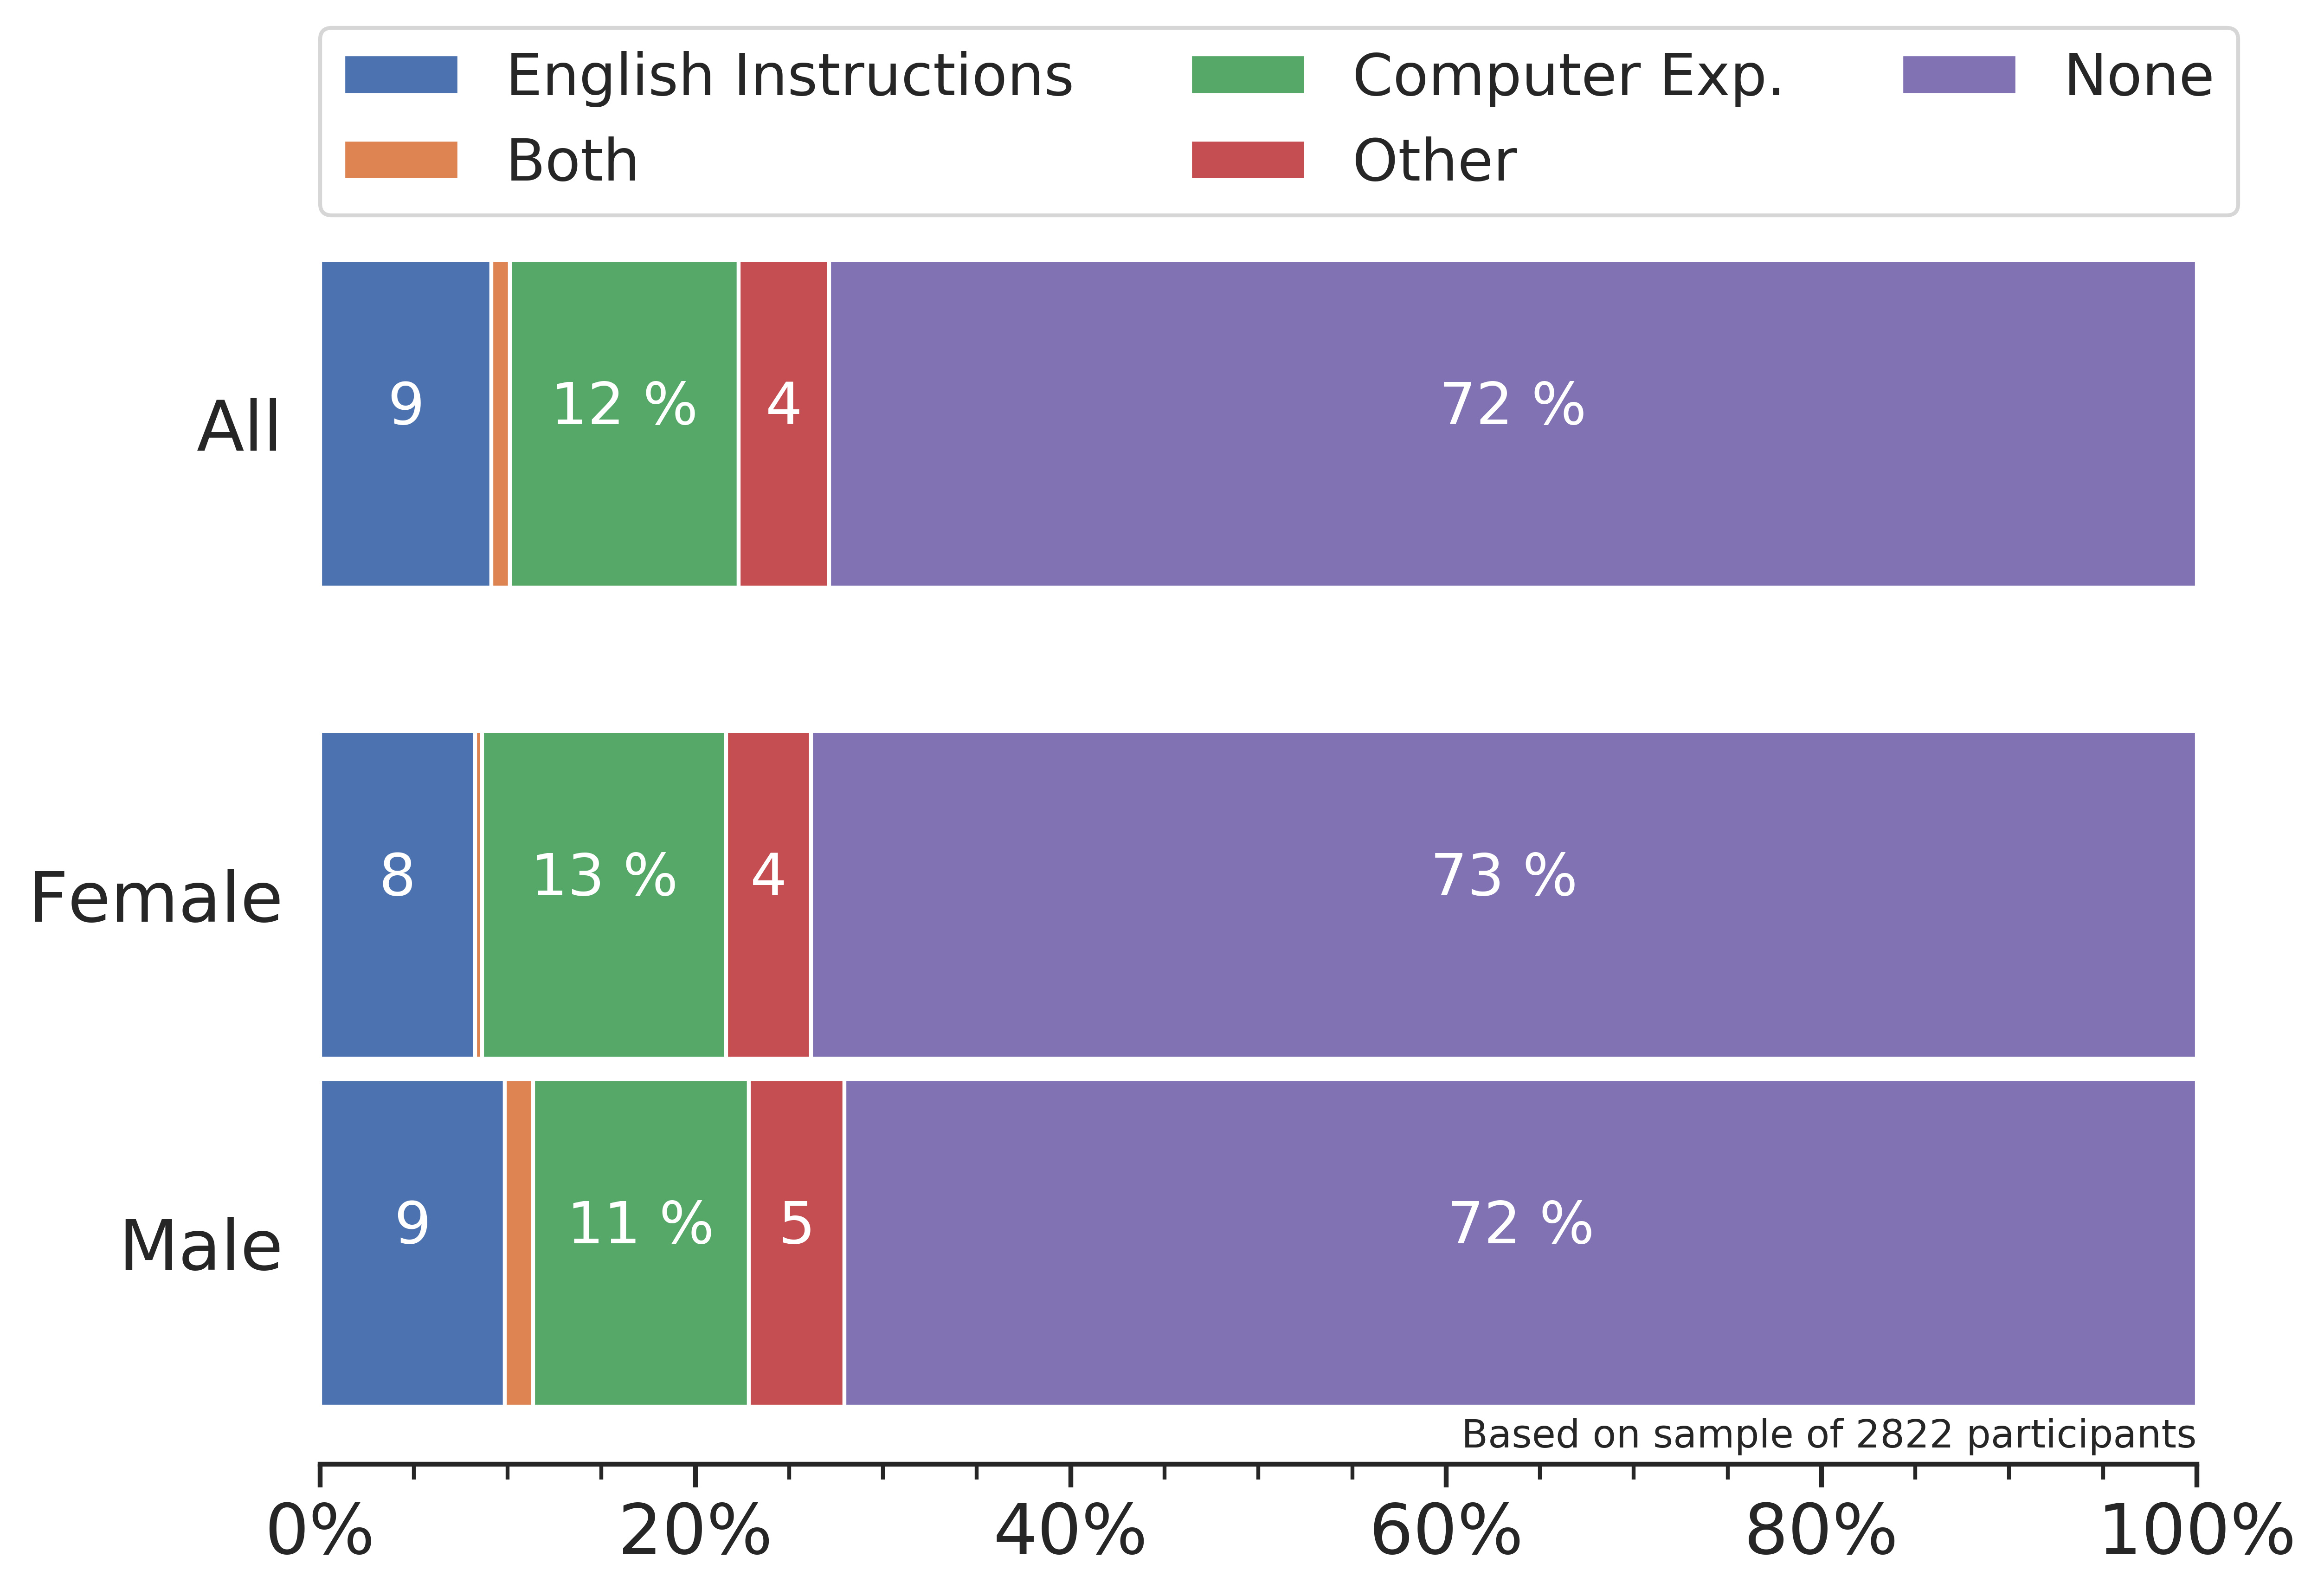
\includegraphics[width=0.7\textwidth]{bar_challenge}
\caption{\small The participants were asked which aspect of their Kano experience was most challenging. The following options were given: ``Understanding and following English language instructions'', ``I am inexperienced in using computers'', ``Other'' and ``None''. This question was used for internal review so we could understand and address the challenges faced by the participants. The data confirmed our empirical observations that those kids new to computers generally struggle most. This question is now retired.} 
\label{fig:challenge}
\end{figure*}

%%%%%%%%%%%%%%%%%%%%%%%%%%%%%%%%%%%%%%%%%%%%%%%%%%%%%%%%%%%%%%%%%%%%%%%%%%%%%%%%%%%%%%%%%%%%%%%%%
%%%%%%%%%%%%%%%%%%%%%%%%%%%%%%%%%%%%%%%%%%%%%%%%%%%%%%%%%%%%%%%%%%%%%%%%%%%%%%%%%%%%%%%%%%%%%%%%%
%%%%%%%%%%%%%%%%%%%%%%%%%%%    Code Club chapter        %%%%%%%%%%%%%%%%%%%%%%%%%%%%%%%%%%%%%%%%%
%%%%%%%%%%%%%%%%%%%%%%%%%%%%%%%%%%%%%%%%%%%%%%%%%%%%%%%%%%%%%%%%%%%%%%%%%%%%%%%%%%%%%%%%%%%%%%%%%
%%%%%%%%%%%%%%%%%%%%%%%%%%%%%%%%%%%%%%%%%%%%%%%%%%%%%%%%%%%%%%%%%%%%%%%%%%%%%%%%%%%%%%%%%%%%%%%%%


\chapter{Code Club}\label{chapter:codeclub}
\graphicspath{{codeclub_plots/}{images/}} % Specifies the directory where pictures are stored




\includegraphics[width=0.7\linewidth, left]{codeclub.jpeg}

Code Clubs are regular structured meetings where a volunteer mentor from the local community assists young people is some coding activities. The aim is to establish a club in as many libraries as possible. These will then meet at least once a week for approximately two hours, during which time participants will be assisted through some coding activities. 

\textit{Code Club}, which is an initiative spearheaded by the \textit{Raspberry Pi Foundation}, provides a complete curriculum covering modules in a variety of programming language, including Python, HTML, Scratch and micro:bit. Upon completion of a module a certificate will be presented to the participants. Libraries Unlimited will also be developing some custom modules based around robotics and climate action accessory kits for the micro:bit, which will be provided to each library. A training boot-camp will be held with the Code Club mentors in order to demonstrate the proper use of these kits.

To date, there are Code Clubs established in 25 district government public libraries with total 231 (106 female \& 125 male) participants meeting regularly. A total of 112 sessions have been completed across these clubs, with four coding languages (Python, HTML \& CSS, Micro:bit and Scratch) being taught. Eight clubs have already completed their first course.

Online Code Clubs were launched in April 2020 to cover the period of library closures due to the Covid-19 pandemic. Two classes are held per week covering a variety of coding languages. As of 15 June 2020, 18 classes have been conducted with a combined total number of 280 participants. 

The Code Club participants complete a general questionnaire when they first join a club and then for each module another questionnaire will be completed at the beginning and the end of the module. The general questionnaire is aimed at measuring attitudinal impacts from the Code Clubs, such as participant's perceived ability to do coding, their interest in coding, whether they believe learning to code will be beneficial to their future careers, etc. The module specific questionnaires are focused on measuring learning outcomes such as the participant's familiarity with core programming concepts. 


\textbf{Data collection is still underway for the Code Clubs, with insufficient data available for an analysis to be presented at this stage. }


%%%%%%%%%%%%%%%%%%%%%%%%%%%%%%%%%%%%%%%%%%%%%%%%%%%%%%%%%%%%%%%%%%%%%%%%%%%%%%%%%%%%%%%%%%%%%%%%%
%%%%%%%%%%%%%%%%%%%%%%%%%%%%%%%%%%%%%%%%%%%%%%%%%%%%%%%%%%%%%%%%%%%%%%%%%%%%%%%%%%%%%%%%%%%%%%%%%
%%%%%%%%%%%%%%%%%%%%%%%%%%%    Do your bit chapter      %%%%%%%%%%%%%%%%%%%%%%%%%%%%%%%%%%%%%%%%%
%%%%%%%%%%%%%%%%%%%%%%%%%%%%%%%%%%%%%%%%%%%%%%%%%%%%%%%%%%%%%%%%%%%%%%%%%%%%%%%%%%%%%%%%%%%%%%%%%
%%%%%%%%%%%%%%%%%%%%%%%%%%%%%%%%%%%%%%%%%%%%%%%%%%%%%%%%%%%%%%%%%%%%%%%%%%%%%%%%%%%%%%%%%%%%%%%%%

\chapter{Do Your Bit}\label{chapter:DYB}
\graphicspath{{doyourbit/}{images/}} % Specifies the directory where pictures are stored


\includegraphics[width=0.7\linewidth, left]{DYBlogo} % Include a department/university logo - this will require the graphicx package

\section{Introduction} % Major section

\href{https://microbit.org/do-your-bit/}{\DYB} is a global micro:bit campaign aimed at inspiring young people to think about how to combine technology and creativity to develop practical solutions to the UN's Sustainable Development Goals (SDGs). The campaign is led by the \textit{Micro:bit Educational Foundation} alongside \textit{ARM}, and \textit{World's Largest Lesson} (in partnership with \textit{Unicef}). With a focus on SDGs 14 and 15, \textit{Life Below Water} and \textit{Life on Land}, the 2019--2020 campaign (which ran until February 2020) encouraged kids to try to solve environmental problems with the micro:bit. Libraries Unlimited have conducted a series of two--day workshops focusing on \DYB in government public libraries across Bangladesh. 

Each workshop included a general introduction to the SDGs, an introduction to the specific SDGs 14 and 15 and a series of micro:bit activities relevant to the particular SDGs. The activities included programming the micro:bit to act as species counter, an anti-poaching collar, a tree protector and an auto--farmer for SDG 15 (\textit{life on land}), and programming the micro:bit as a guiding light for sea--turtle hatchlings, a bright and loud device to attach to a fishing net to avoid by--catch, an ocean health monitor and a prototype oil spill cleaner for SDG 14 (\textit{life below water}). 

These activities were spread over two full days with the same group of participants. Note that the first workshop was one day-long, but this proved to be insufficient time to cover the necessary material. 

At beginning and end of each workshop a pre- and post- questionnaire was distributed to each participants to complete. The results in this report are generated from an analysis of these forms.



\subsection{The Key Aims:}

The key aims for the \DYB campaign within Libraries Unlimited is to:
\begin{itemize}
\item Inspire a desire to do coding and provide a more in-depth coding experience to young people (relative to the introductory coding workshops).
\item Develop problem solving skills and creative thinking in the service users.
\item Educate people about the SDGs.
\item Inspire young people to think about how coding and technology can be applied practically in the real-world.
\item Educate people to better understand how technology works, develop computational thinking and inspire future tech innovators.
\item Increase the scope of the activities available within the public library network and attract more users to the libraries.
\end{itemize}

%------------------------------------------------

\section{Workshop Details} % Sub-section

Libraries Unlimited has conducted three \DYB workshops in Govt. District Public Libraries in Bangladesh as part of the 2019--2020 campaign. An overview of the workshops held is presented in Table~\ref{tab:DYBworkshops}.% and a map indicating the locations of library based workshops to date is presented in Figure~\ref{fig:map}.

\begin{table}[ht] 
\centering % Centres the table on the page, comment out to left-justify
\begin{tabular}{l l c c c c} % The final bracket specifies the number of columns in the table along with left and right borders which are specified using vertical pipes (|); each column can be left, right or center-justified using l, r or c. Columns will widen to hold the content in them by default, to specify a precise width, use p{width}, e.g. p{5cm}
\hline % Top horizontal line
\# & Location & Date & \multicolumn{3}{c}{Number of Participants:}\\ % Amalgamating several columns into one cell is done using the \multicolumn command with the number of columns to amalgamate as the first argument and then the justification (l, r or c)
%\cmidrule(l){3-5} % Horizontal line spanning less than the full width of the table - you can add (r) or (l) just before the opening curly bracket to shorten the rule on the left or right side
&&& Total & Female & Male\\ % Column names row
\hline
\hline
1 & Sufia Kamal National Library & 24/09/2019 & 16 & 6 & 10\\
2 & Coxs Bazar Public Library & (16\,\&\,17)/11/2019 & 23 & 14 & 9\\
3 & Mymensingh Public Library & (11\,\&\,12)/01/2020 & 21 & 0 & 21\\

\hline % In-table horizontal line
 && \textbf{Total} & \textbf{60} & \textbf{20} & \textbf{40}\\ % Summary/total row
\hline% Bottom horizontal line
\end{tabular}
\caption{Details on the workshops held to date.} % Table caption, can be commented out if no caption is required
\label{tab:DYBworkshops} % A label for referencing this table elsewhere, references are used in text as \ref{label}
\end{table}
%------------------------------------------------

%\begin{figure}[!htb] % Example image
%\center{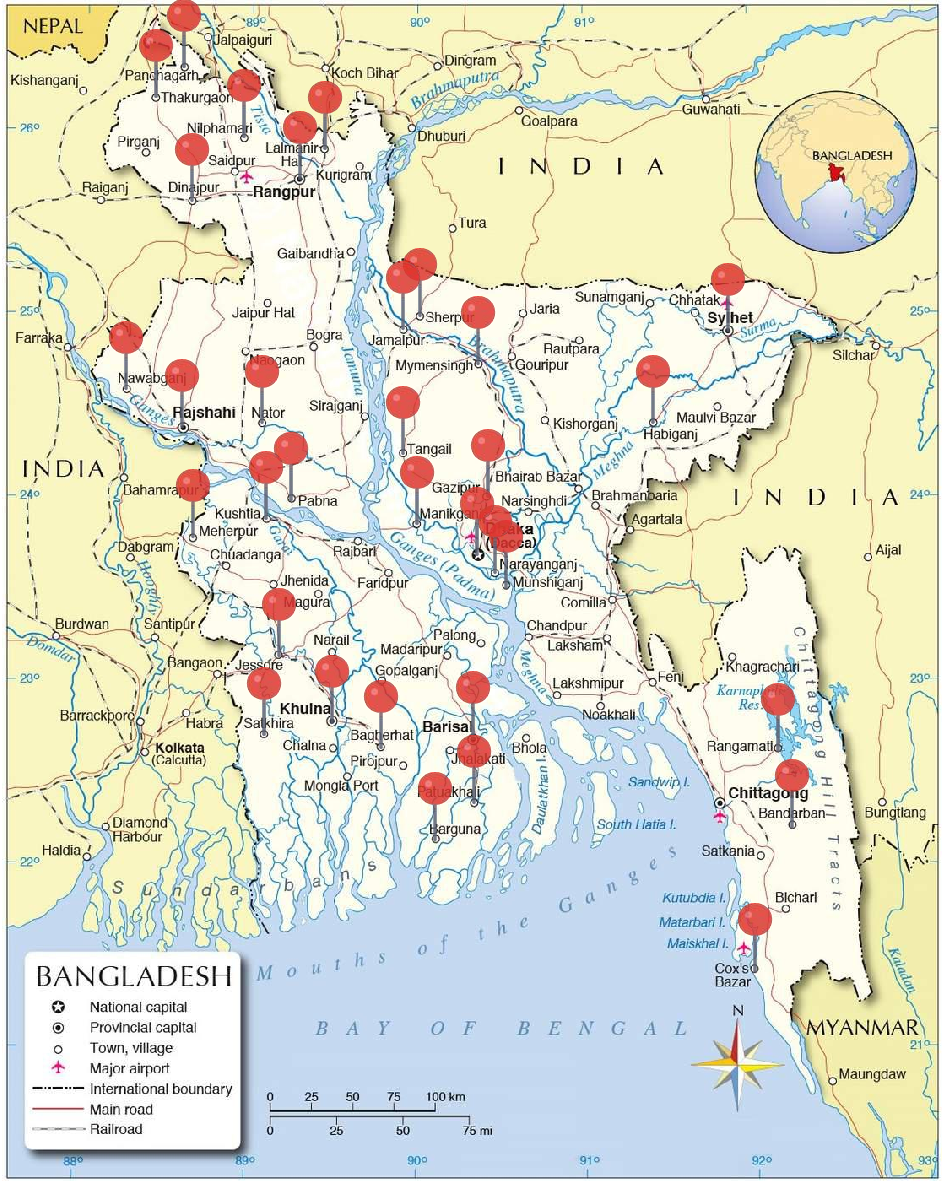
\includegraphics[width=0.99\linewidth]{PinnedMap-crop}}
%\caption{Map of Bangladesh with the location of held workshops pinned.}
%\label{fig:map}
%\end{figure}

%------------------------------------------------

\begin{figure*}[t!]
    \centering
    \begin{subfigure}[]{0.46\textwidth}
        \centering
        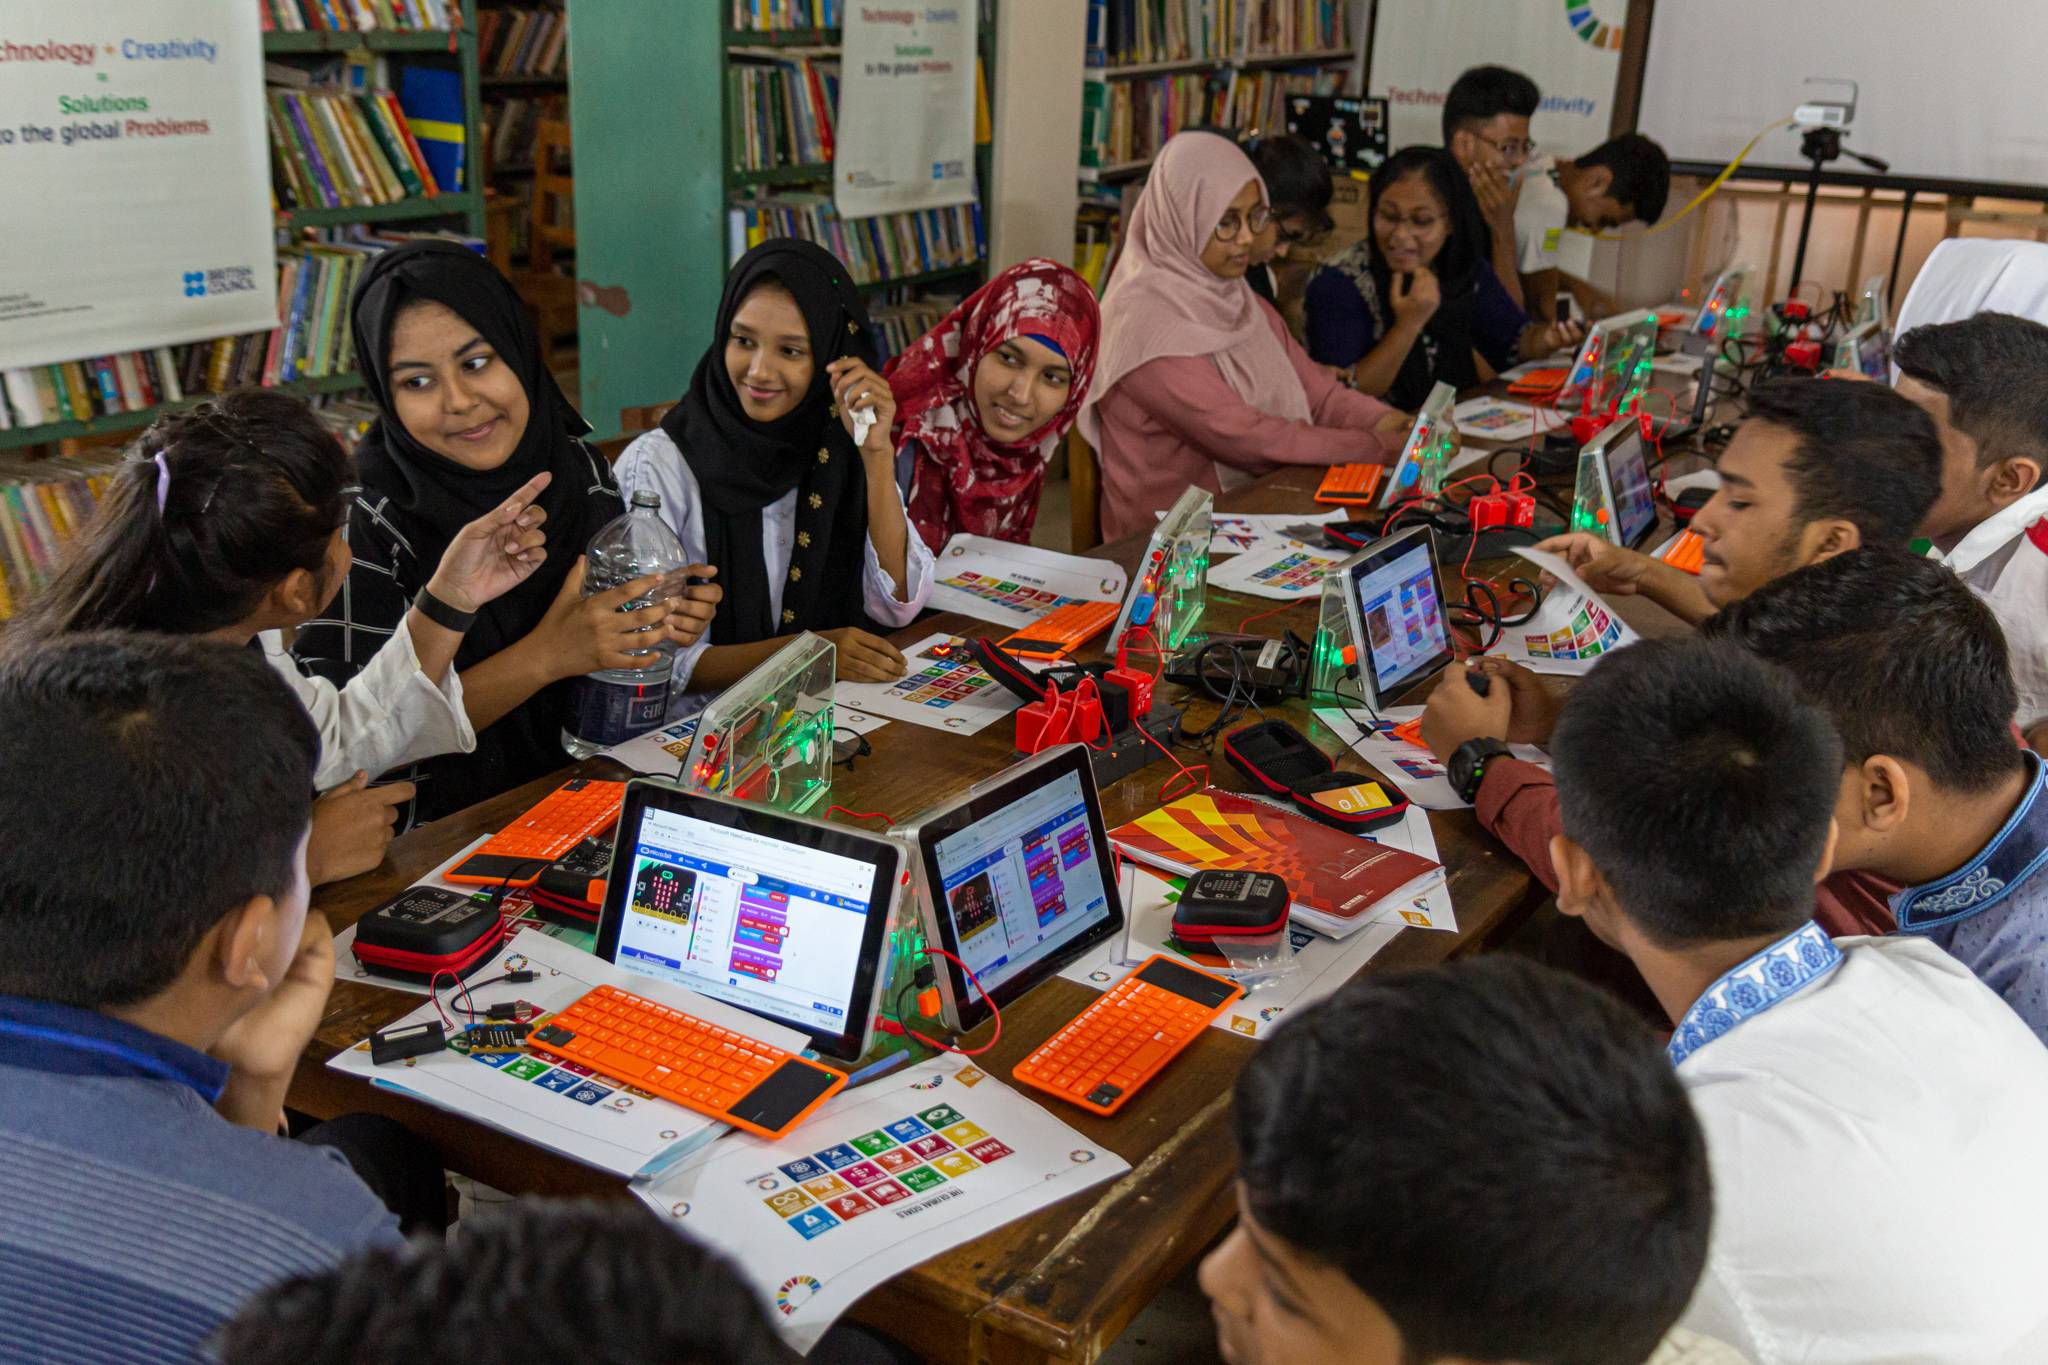
\includegraphics[width=1.0\textwidth]{dyb_coxsbazar_s_22}
    \end{subfigure}
    \begin{subfigure}[]{0.46\textwidth}
        \centering
        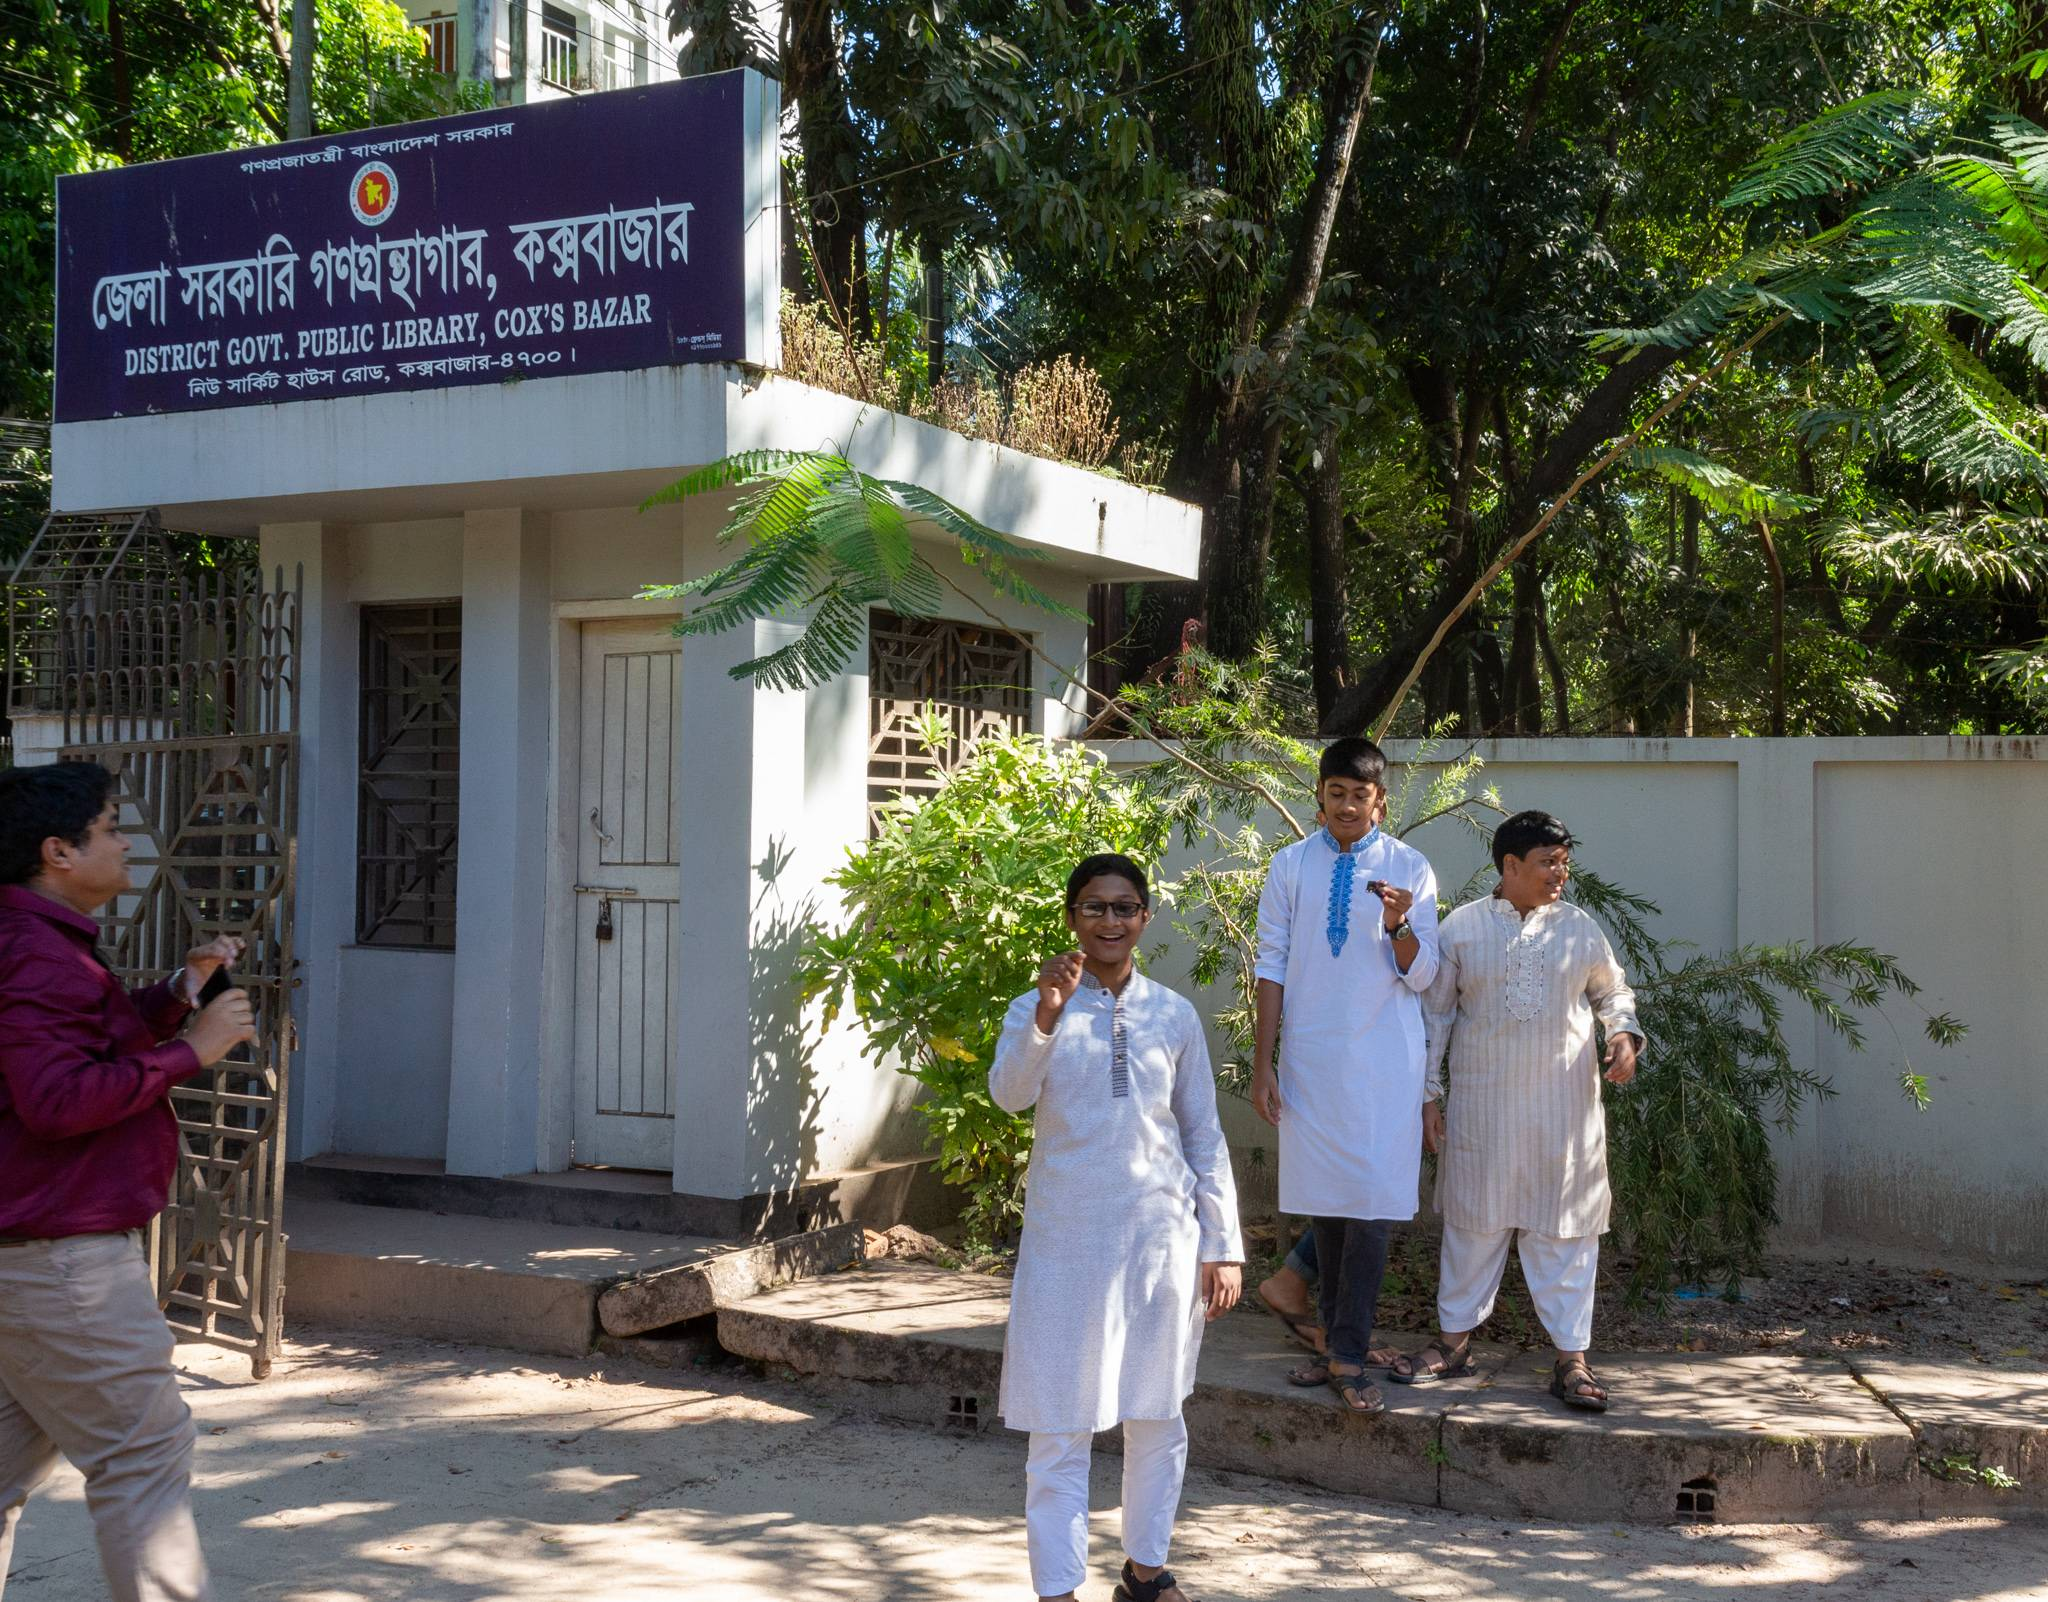
\includegraphics[width=1.0\textwidth]{dyb_coxsbazar_s_17}
    \end{subfigure}

        \begin{subfigure}[]{0.46\textwidth}
        \centering
        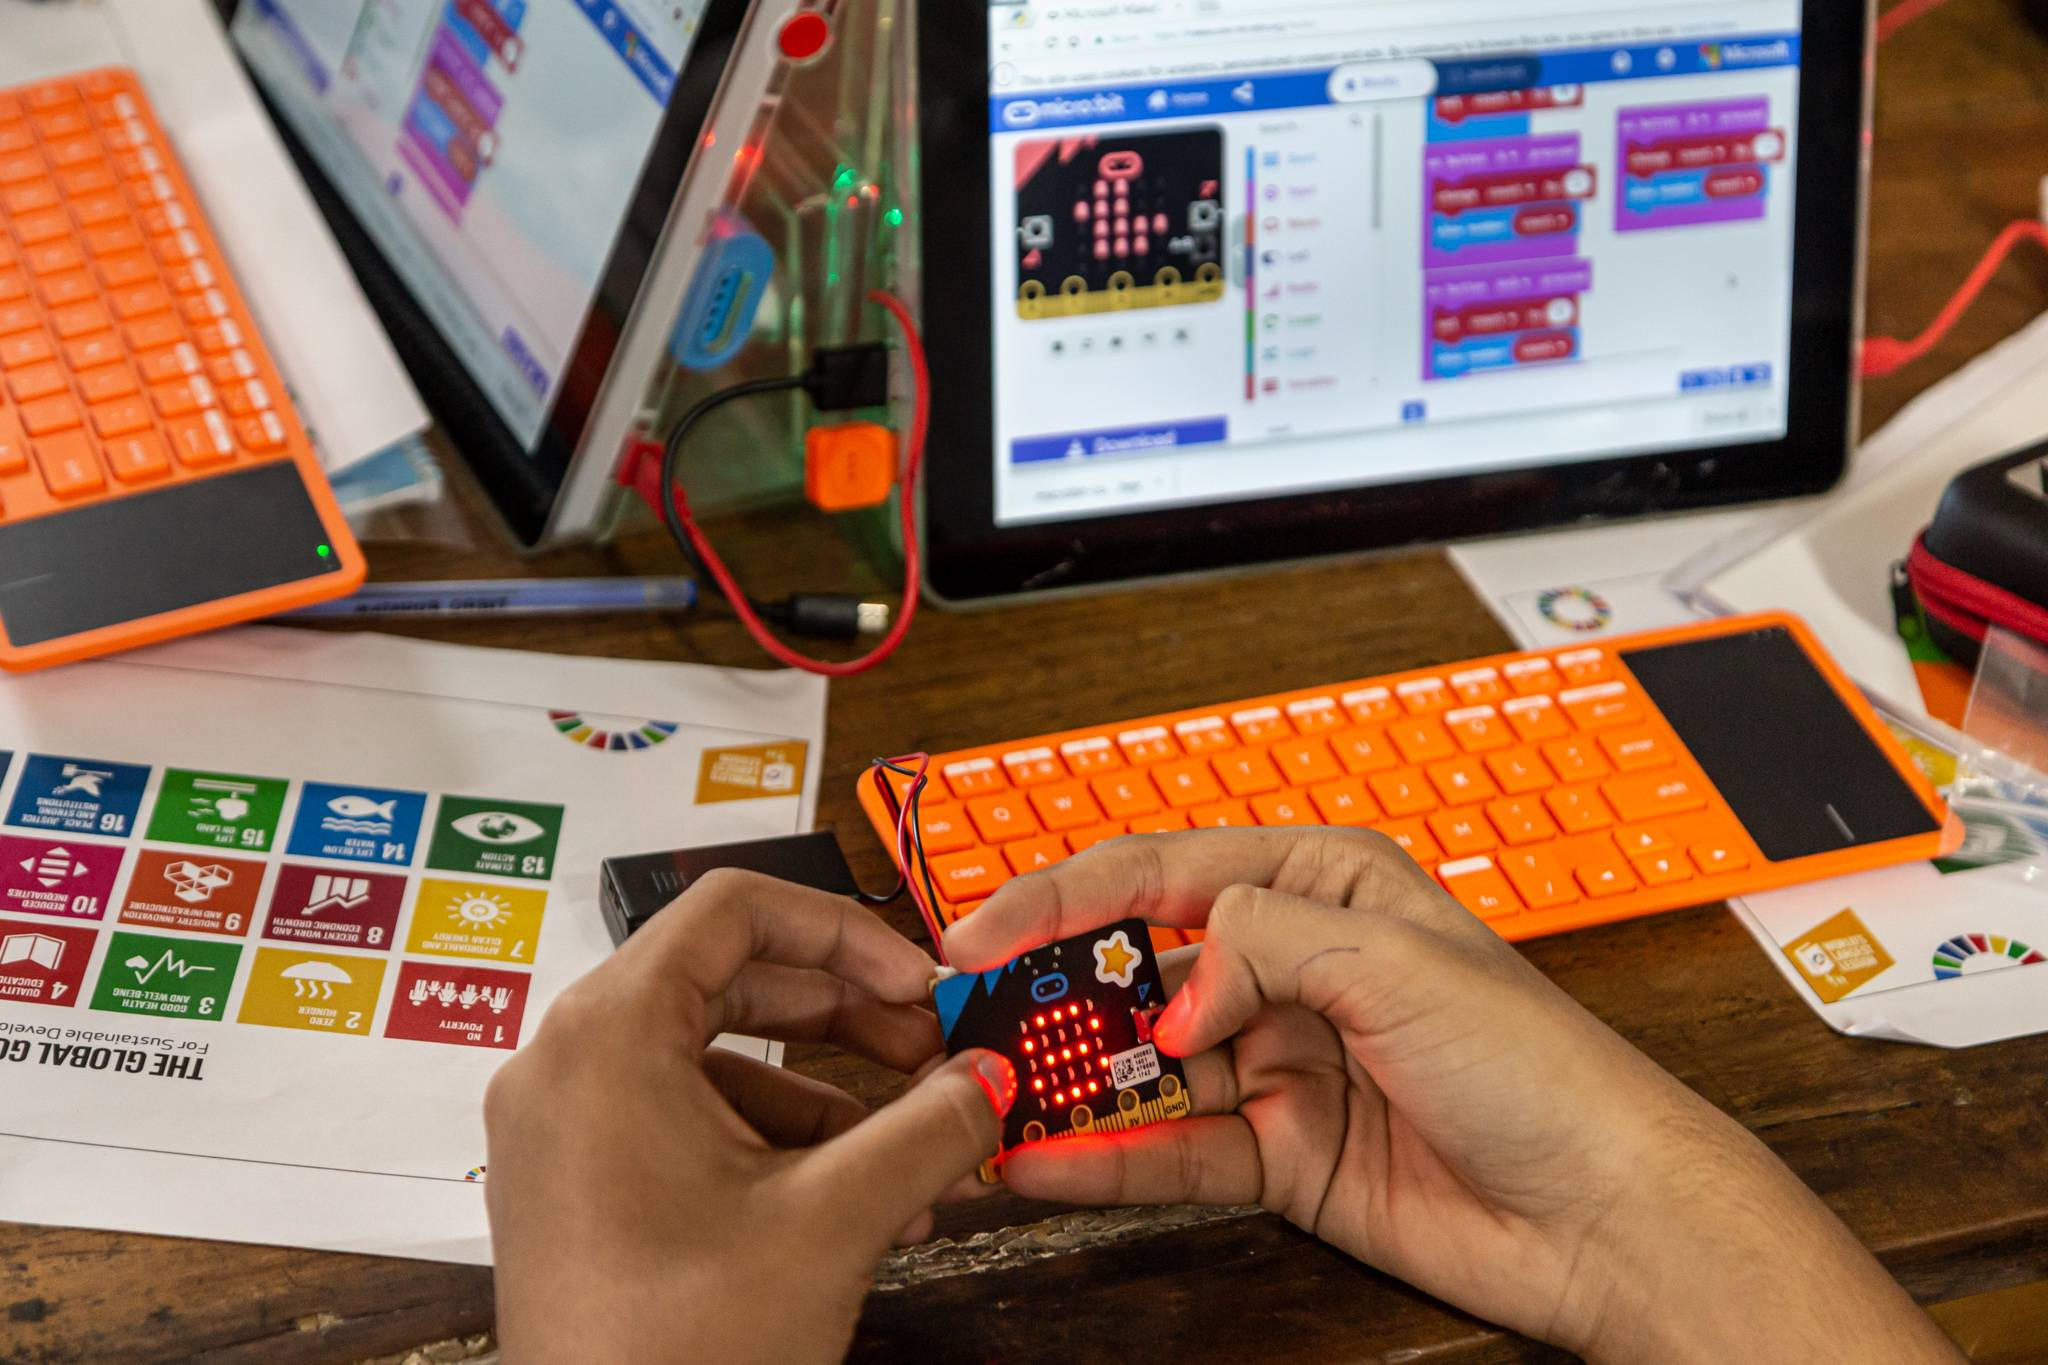
\includegraphics[width=1.0\textwidth]{dyb_coxsbazar_s_23}
    \end{subfigure}
    \begin{subfigure}[]{0.46\textwidth}
        \centering
        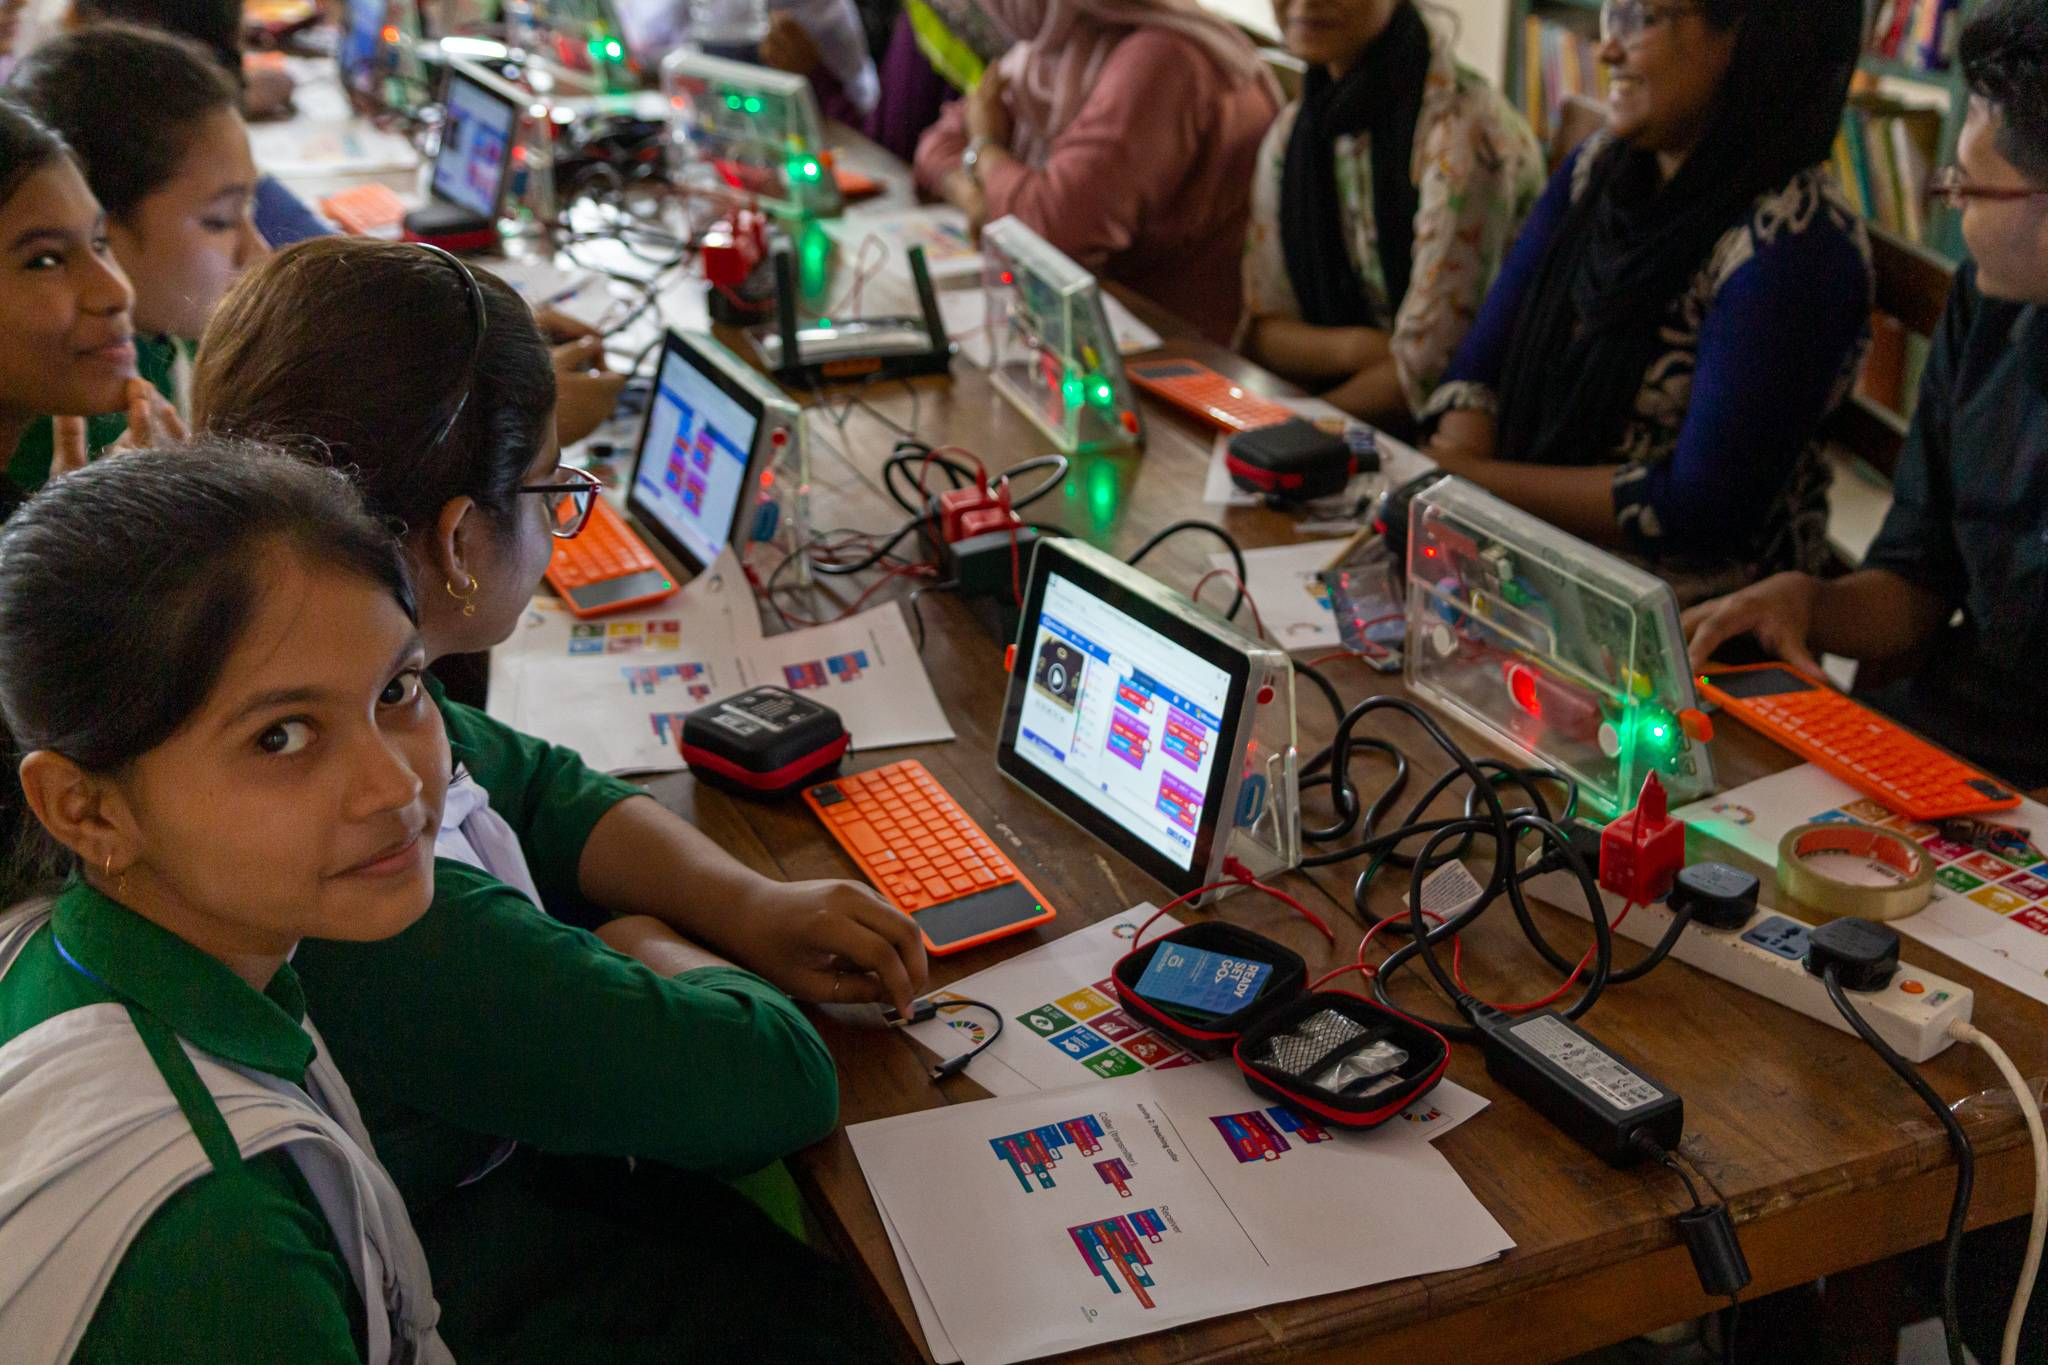
\includegraphics[width=1.0\textwidth]{dyb_coxsbazar_s_25}
    \end{subfigure}

   
        \begin{subfigure}[]{0.46\textwidth}
        \centering
        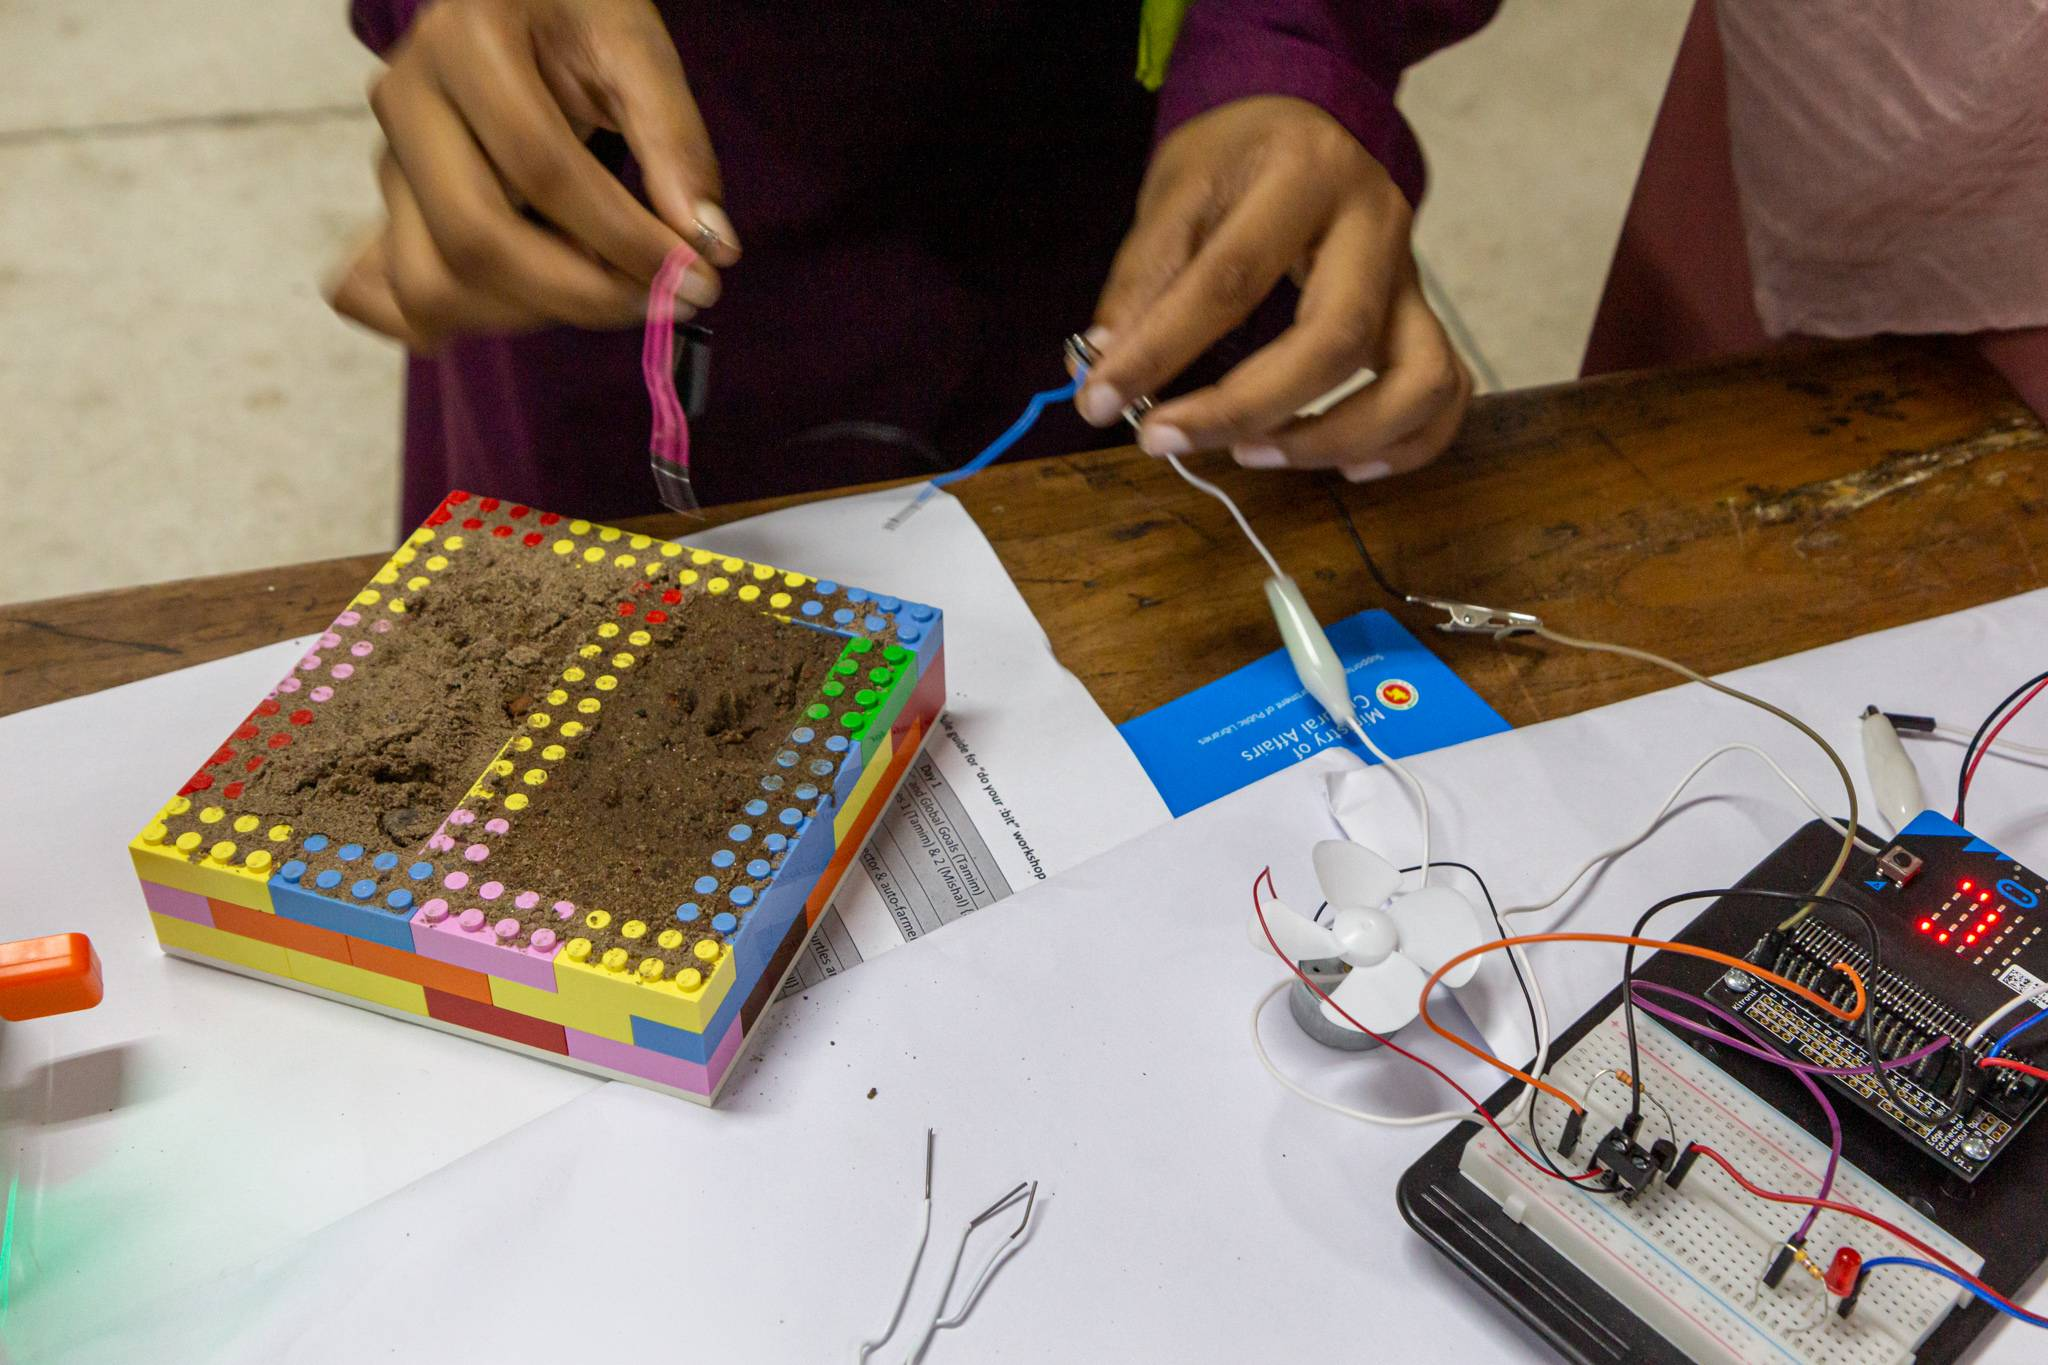
\includegraphics[width=1.0\textwidth]{dyb_coxsbazar_s_28}
    \end{subfigure}
    \begin{subfigure}[]{0.46\textwidth}
        \centering
        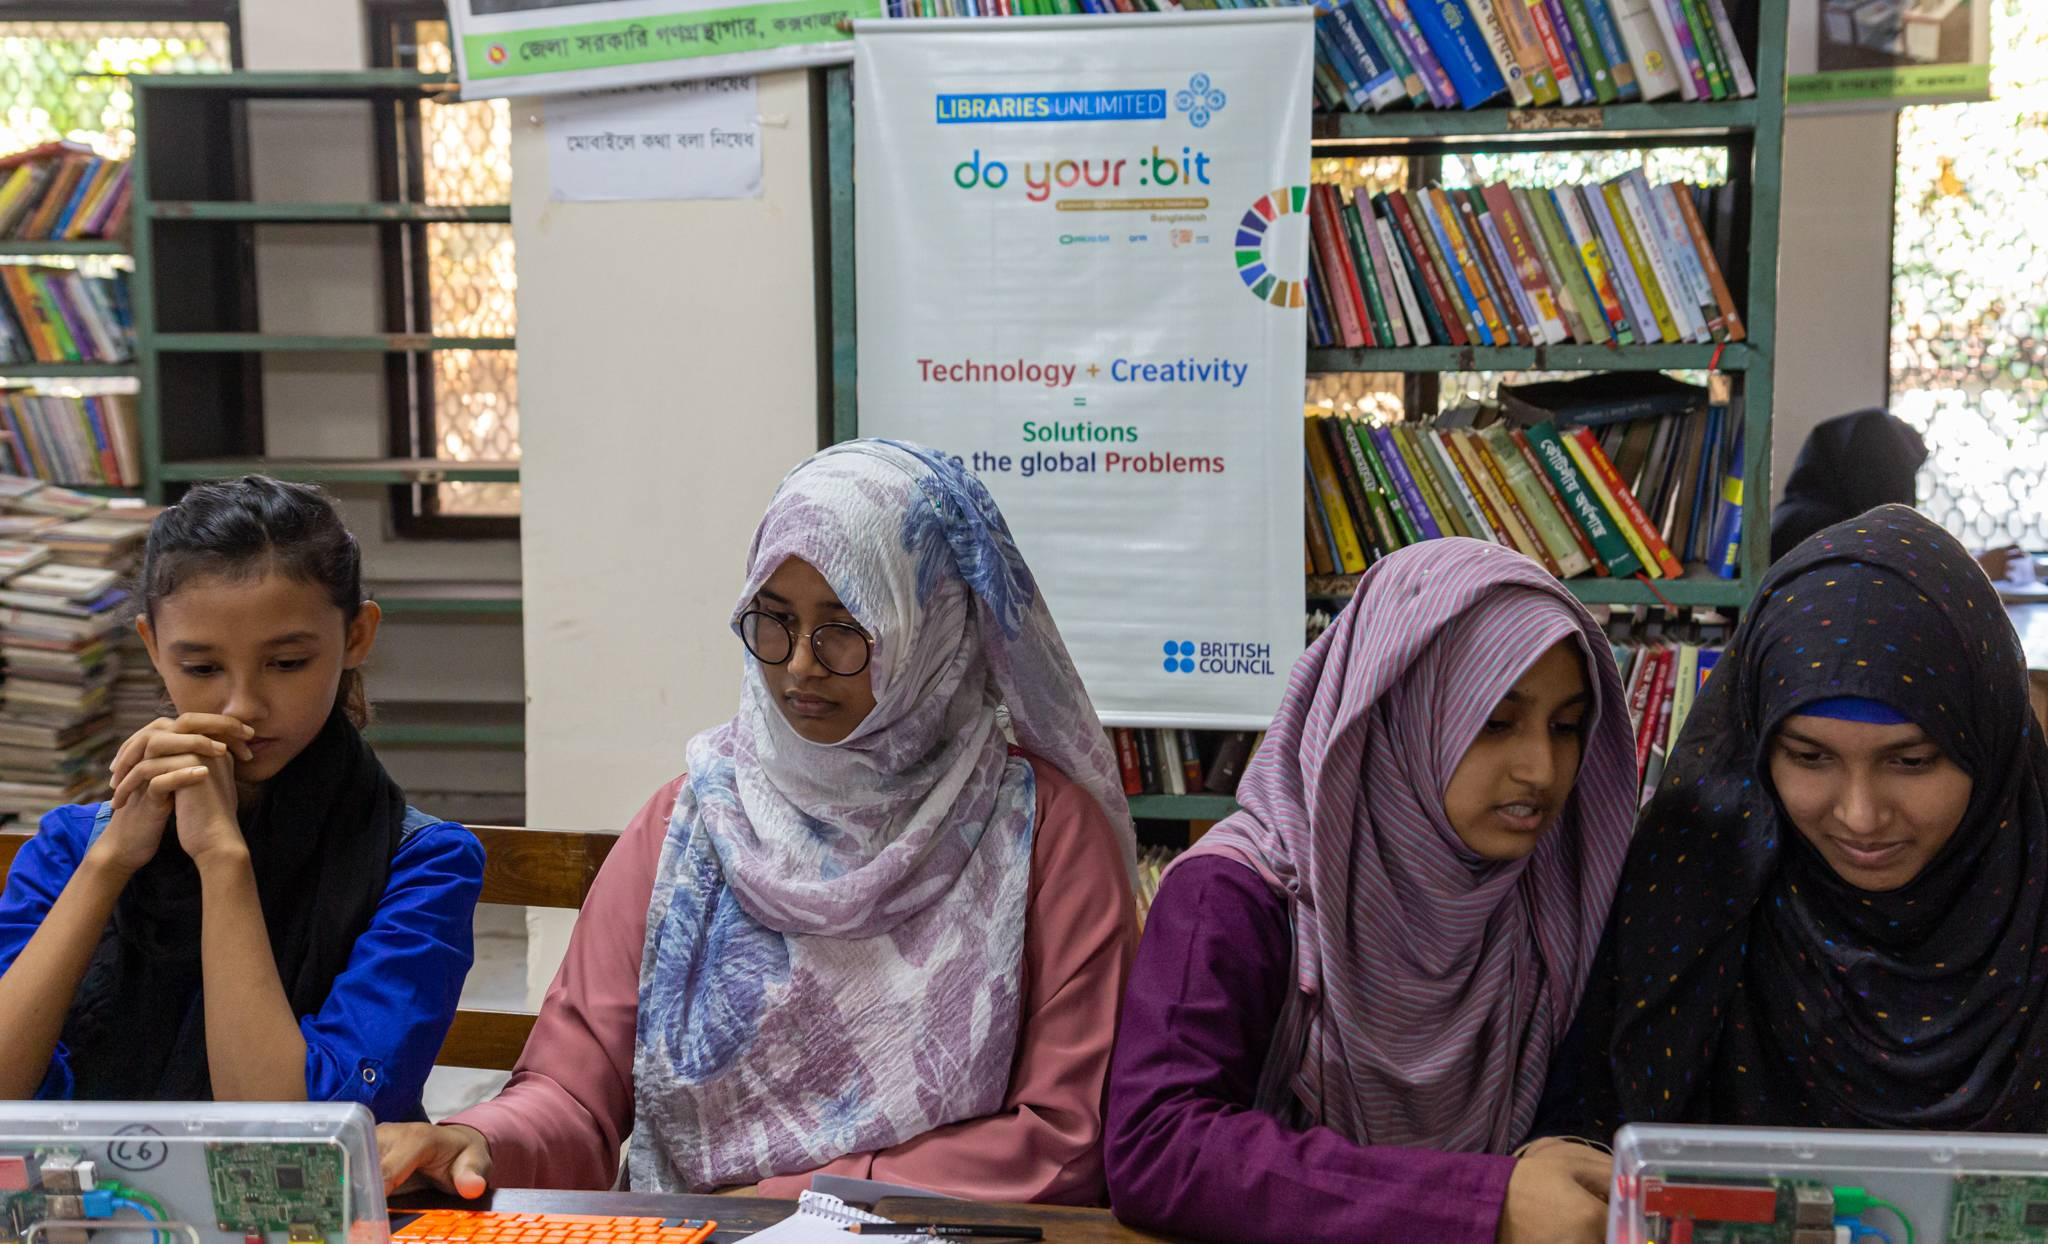
\includegraphics[width=1.0\textwidth]{dyb_coxsbazar_s_32}
    \end{subfigure}
    
        \begin{subfigure}[]{0.46\textwidth}
        \centering
        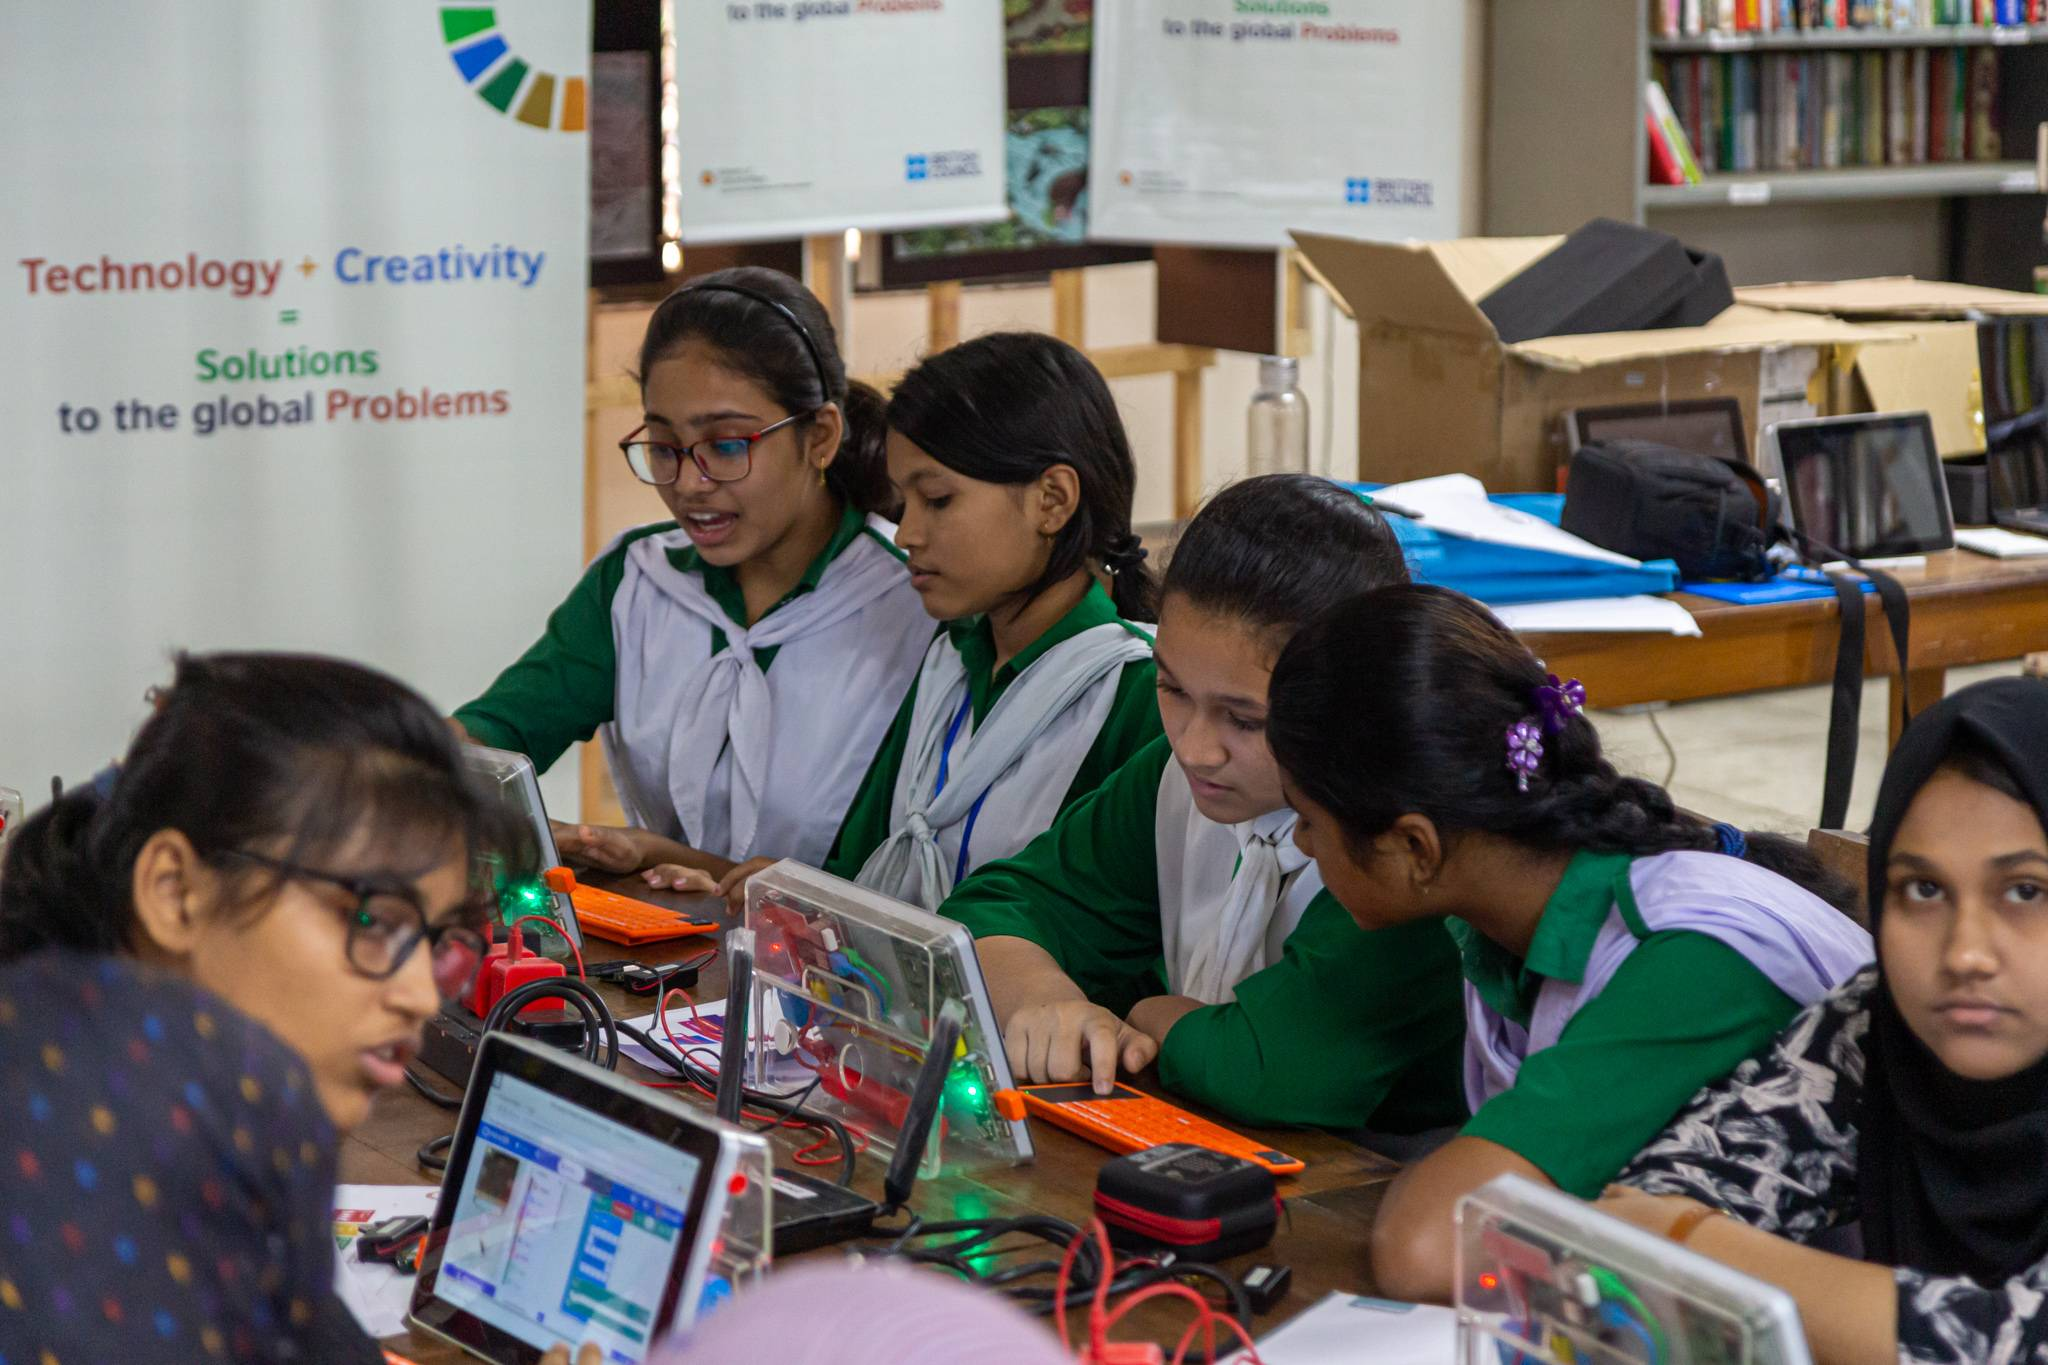
\includegraphics[width=1.0\textwidth]{dyb_coxsbazar_s_40}
    \end{subfigure}
    \begin{subfigure}[]{0.46\textwidth}
        \centering
        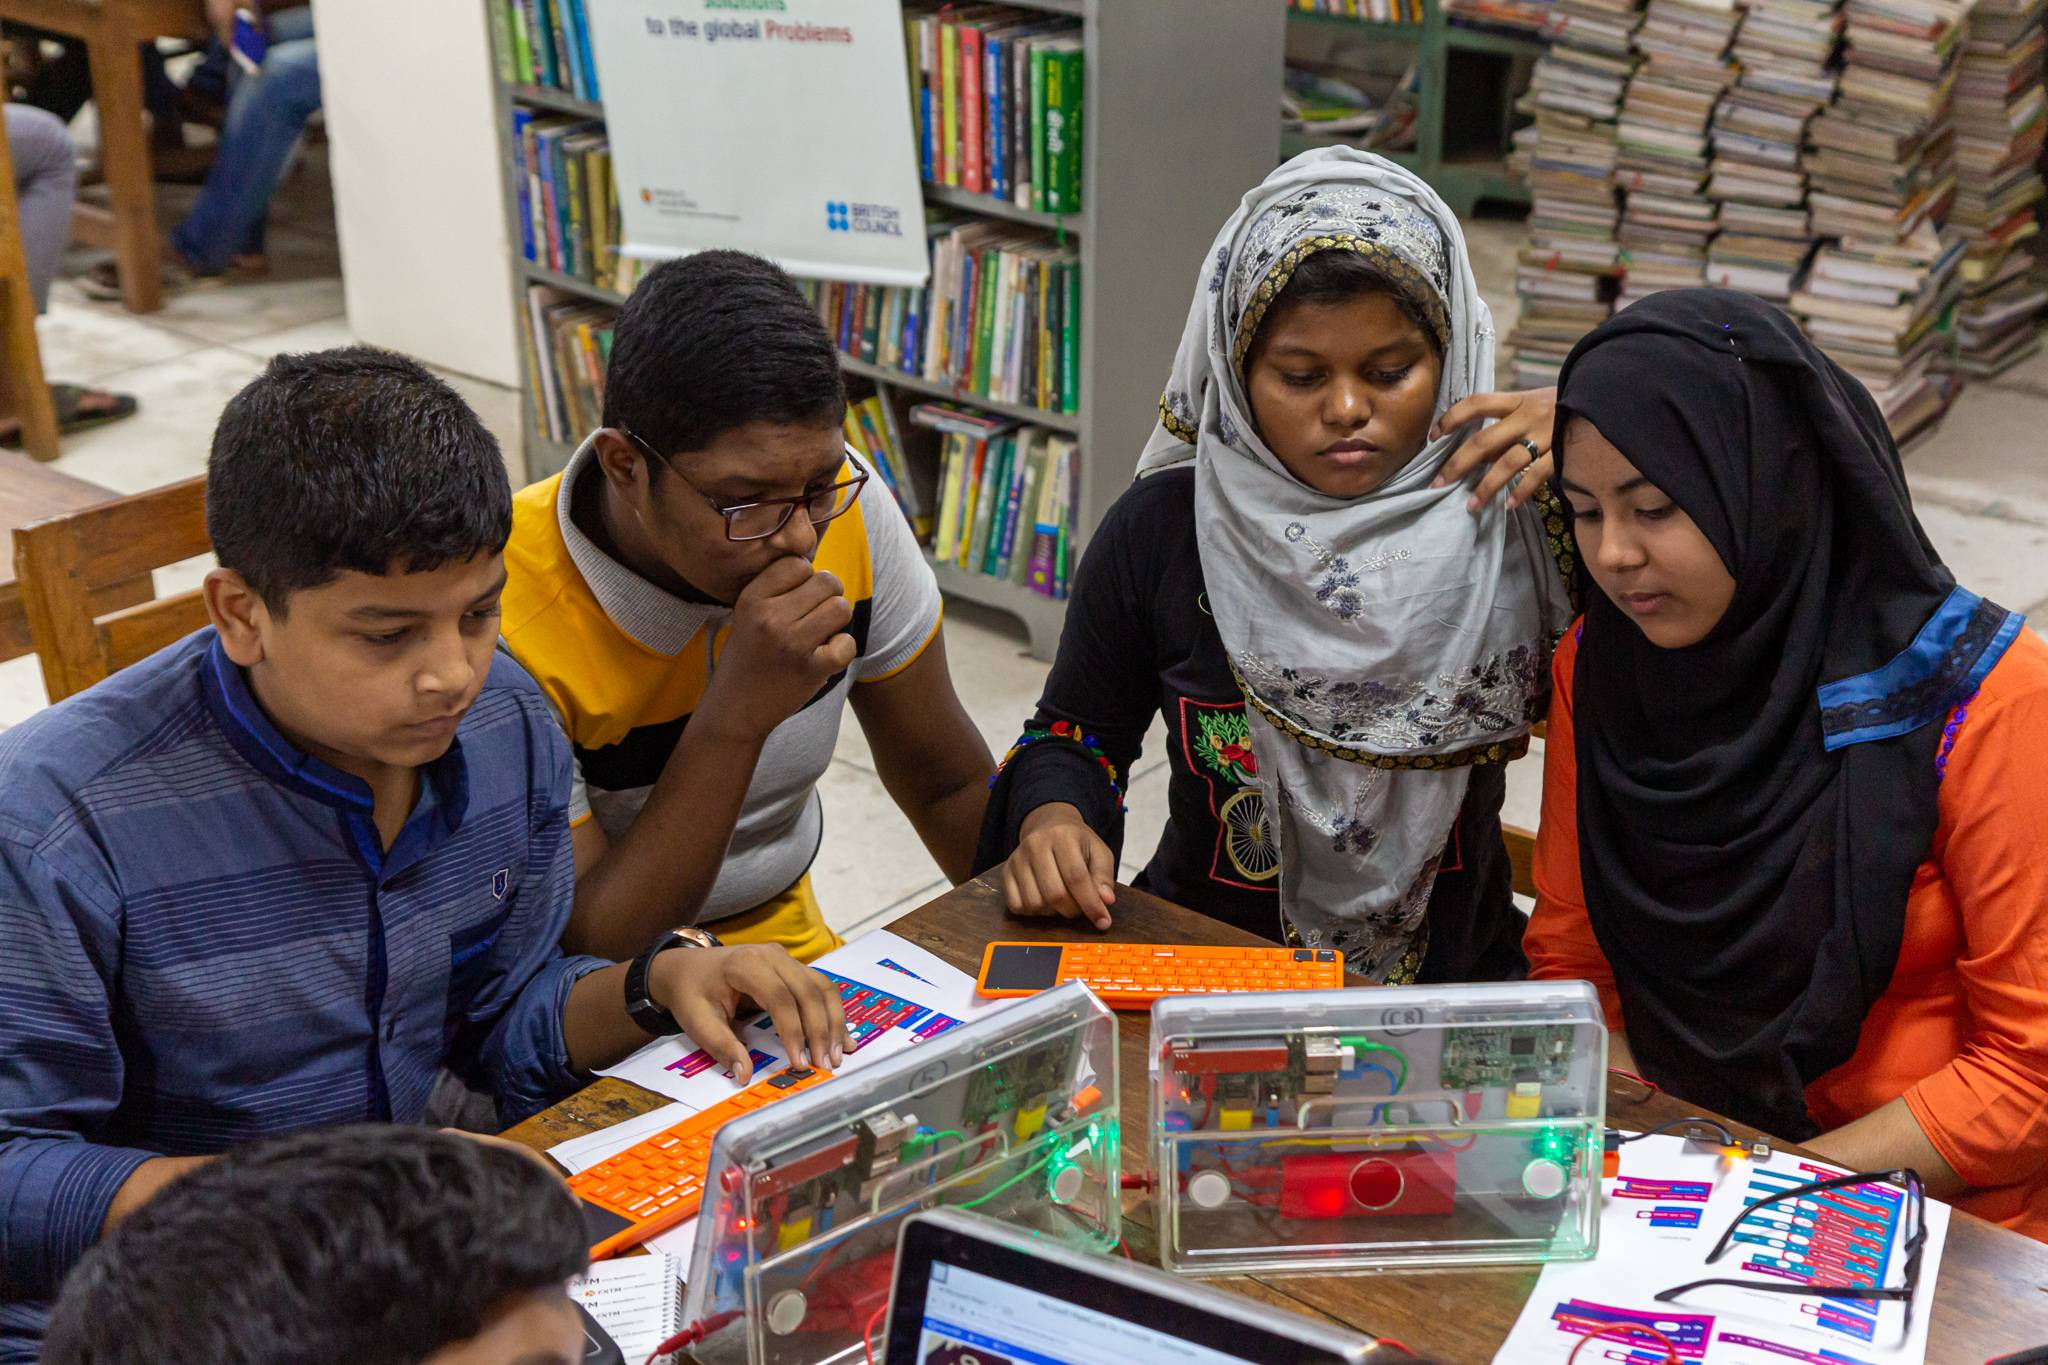
\includegraphics[width=1.0\textwidth]{dyb_coxsbazar_s_41}
    \end{subfigure}    
    \caption{A selection of photos from the Dhaka and Cox's Bazar \DYB library workshops.}
    \label{fig:photos}
\end{figure*}

\newpage
%------------------------------------------------
\subsection{Participant Demographics} % Sub-sub-section

The gender distribution of the participants was two thirds male and one third female (see Figure~\ref{fig:DYBgender}). This is unfortunately skewed toward boys because of the all male participants at the Mymensingh workshop. However, invitation of the kids is in the remit of the librarians and the schools have the decision regarding which students to bring.   

\begin{figure}% Example image
\center{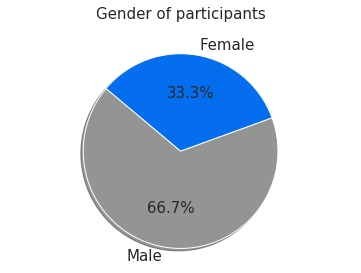
\includegraphics[width=0.6\linewidth]{pie_gender}}
\caption{The gender distribution of participants at the \DYB workshops.}
\label{fig:DYBgender}
\end{figure}

%------------------------------------------------

See Figure~\ref{fig:DYBage} for the age distribution of participants. The vast majority ($85$ per cent) of participants were aged 12 to 15, with a median age of 14. Note that this is by design as we communicate this as the desired age range when planning the workshops.  

\begin{figure} % Example image
\center{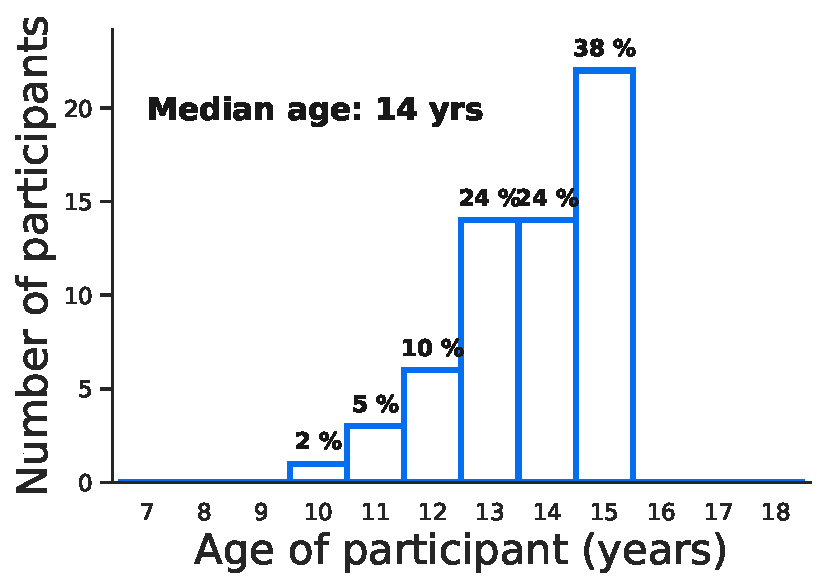
\includegraphics[width=0.7\linewidth]{AgeDistribution}}
\caption{The age distribution of participants at the \DYB workshops.}
\label{fig:DYBage}
\end{figure}

%----------------------------------------------------------------------------------------
%	MAJOR SECTION 1
%----------------------------------------------------------------------------------------

\goodbreak
\section{Feedback Results} % Major section
This section will explore the results of the feedback collected. %Figure~\ref{fig:quotes} provides a selection of written comments from participants. 
Figures~\ref{fig:DYBworkshopexp}--\ref{fig:sdgimportant} graphically illustrate feedback results. A summary of the key results is given here:
\begin{itemize}
\item We asked the participants to rate their overall experience of the workshop. The results were positive: 88 per cent said it was very good and the remaining 12 per cent said good (see Figure~\ref{fig:DYBworkshopexp}).

\item The workshop substantially improved the confidence of the participants in their ability to do coding. Prior to the workshop only 34 per cent of participants felt they were able to do coding, 33 per cent of participants answered that were unable to do coding and 33 per cent didn't know whether they could. Following the workshop, 88 per cent felt they were able to do coding, only 12 per cent were unsure and zero participants felt unable to do coding (see Figure~\ref{fig:DYBcandocoding}).

\item The workshop increased the level of interest in the participants towards coding. Prior to the workshops, 24 per cent of participants were unsure or not interested in coding, whereas after the workshop this dropped to nine per cent. The proportion of participants who are very interested in doing coding increased from 48 per cent before the workshop to 78 per cent after (see Figure~\ref{fig:DYBcodinginterest}). 

 \item Prior to the workshop there was a high awareness of the potential to use technology to solve problems with 91 per cent of participants answering they believe technology can be used to solve environmental problems. The workshop increased this awareness further to 98 per cent after the workshop (see Figure~\ref{fig:techsolve}). 
 
\item There was an initial high awareness of the SDGs in general amongst the participants, with 83 per cent of participants saying they are have heard of the SDGs prior to the workshop. After the workshop this had increased to 100 per cent (see Figure~\ref{fig:knowsdgs}). 

\item Awareness of the specific SDGs 14 and 15 were substantially improved by the workshop. The proportion of participants who said they did not know about either SDG 14 and 15 decreased from 74 per cent before the workshop to seven per cent after the workshop (see Figure~\ref{fig:knowsdg1415}).

\item The workshop increased the perception of the importance of the SDGs in the participants. After the workshop 84 per cent felt the SDGs are very important compared to 63 per cent before the workshop. The proportion who were unsure or thought they are unimportant decreased from 14 per cent before the workshop to seven per cent after the workshop (see Figure~\ref{fig:sdgimportant}).
  \end{itemize}


%\begin{figure*}[t!]
%    \centering
%        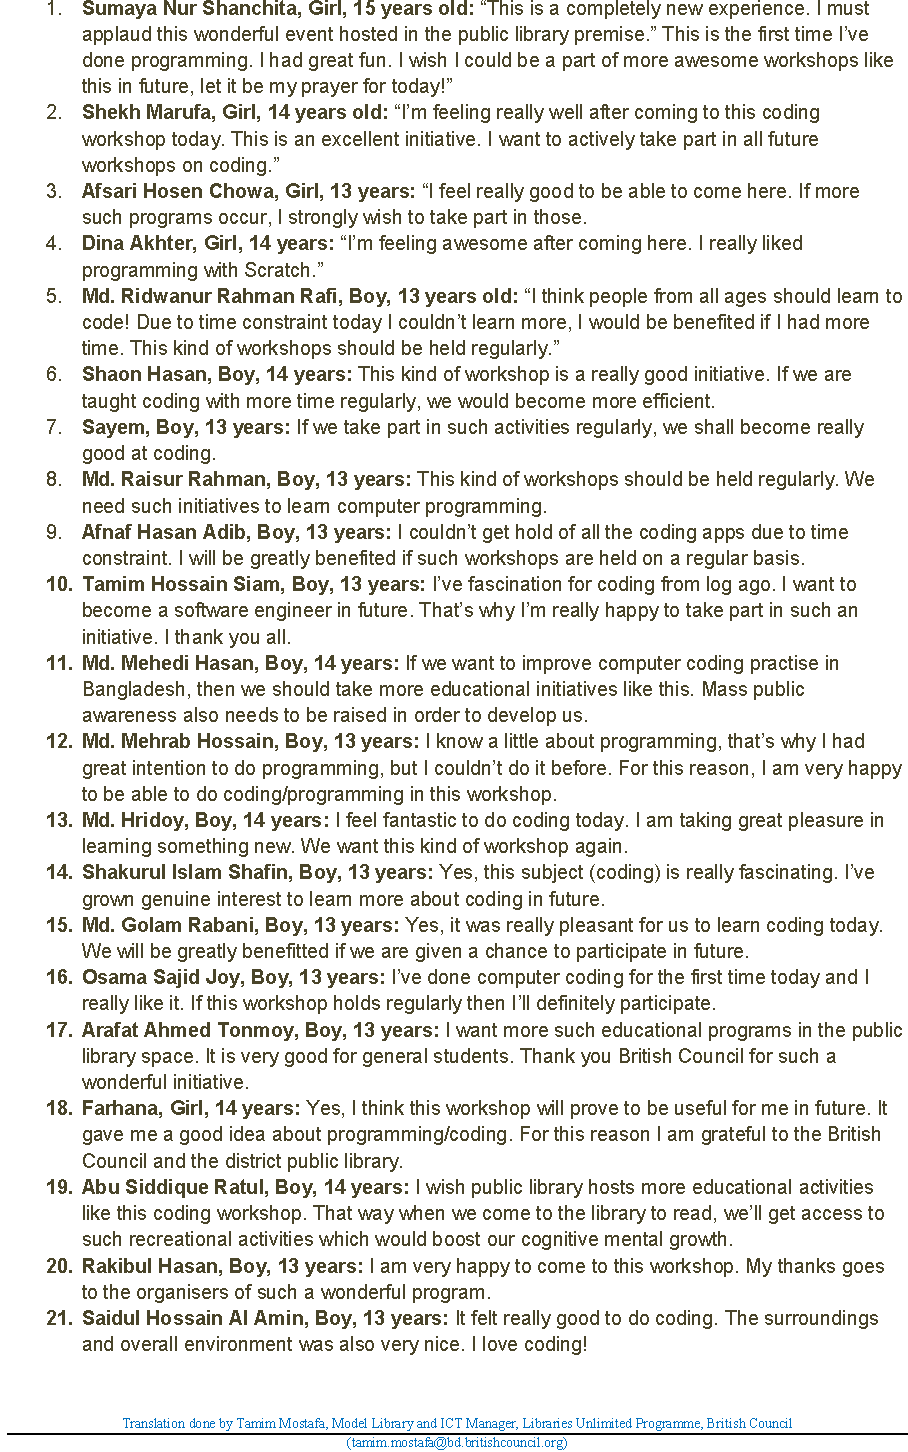
\includegraphics[width=1\textwidth]{quotes-crop}
%\caption{A selection of written comments collected on the feedback forms.  } 
%\label{fig:quotes}
%\end{figure*}


\begin{figure*}[t!]
    \centering
        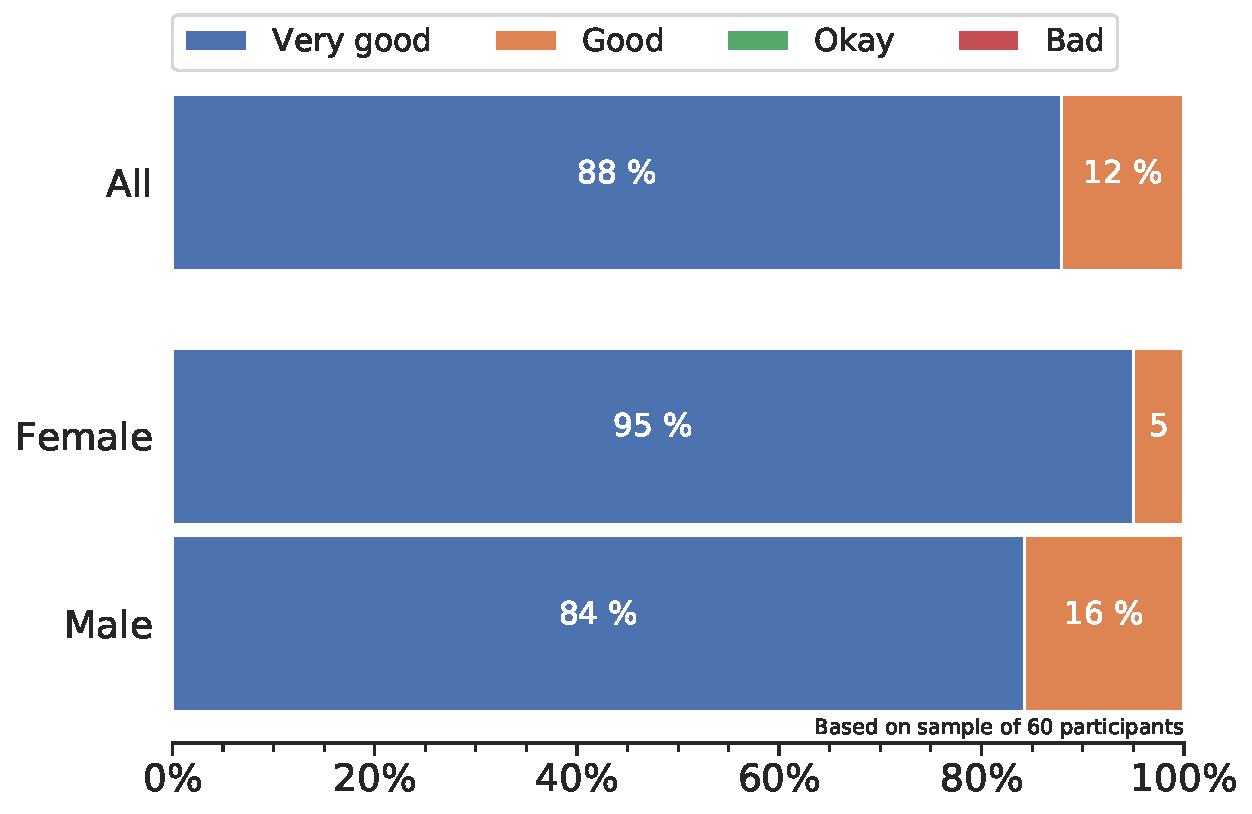
\includegraphics[width=0.85\textwidth]{bar_workshopexp}
    \caption{The \DYB participants were asked to rate their overall experience of the workshop. The feedback was very positive with 88 per cent saying it was very good, 12 per cent saying good and no one saying it was only okay or bad. }
    \label{fig:DYBworkshopexp}
\end{figure*}


\begin{figure*}[t!]
    \centering
        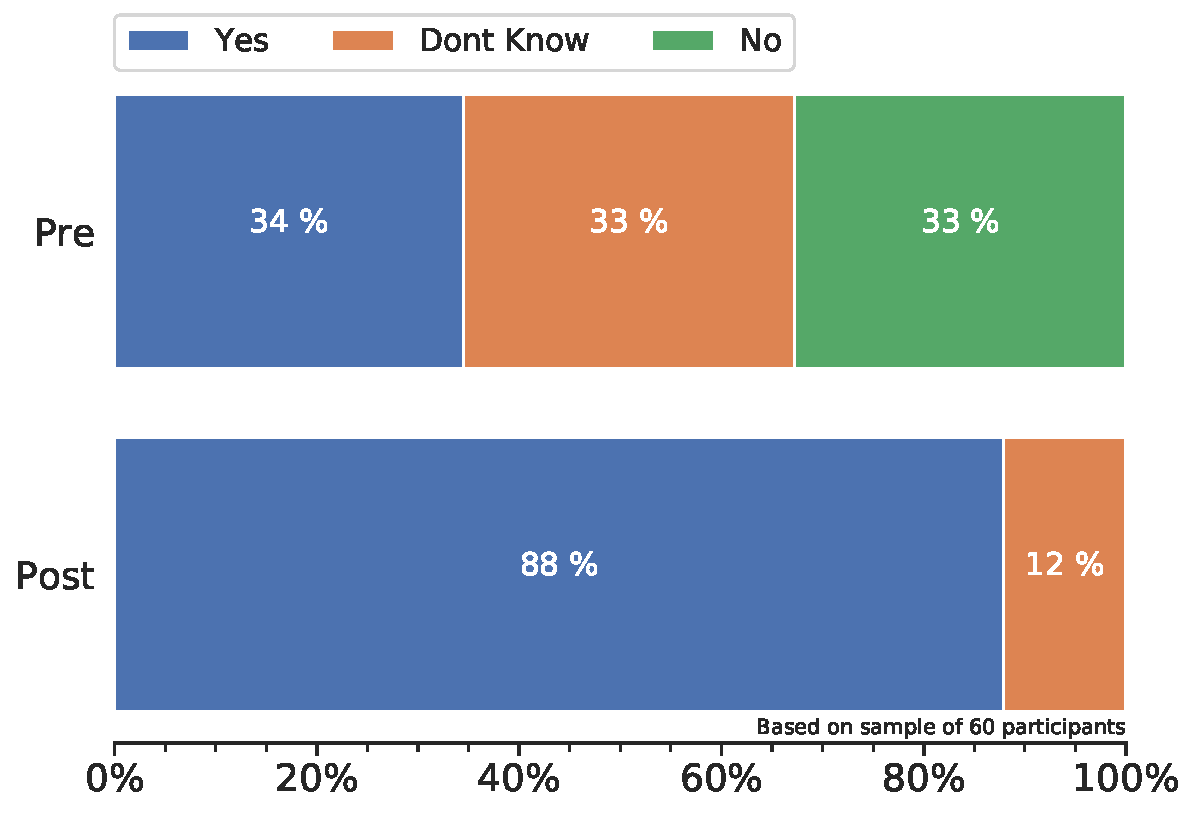
\includegraphics[width=0.85\textwidth]{bar_candocoding}
\caption{The \DYB participants were asked before and after the workshop whether they believed they could do coding. There is a clear increase in confidence for the participants and their perceived ability to do coding. Prior to the workshop only 34 per cent of participants felt they were able to do coding, 33 per cent of participants answered that were unable to do coding and 33 per cent didn't know whether they could. Following the workshop, 88 per cent felt they were able to do coding, only 12 per cent were unsure and zero participants felt unable to do coding.} 
\label{fig:DYBcandocoding}
\end{figure*}


\begin{figure*}[t!]
    \centering
        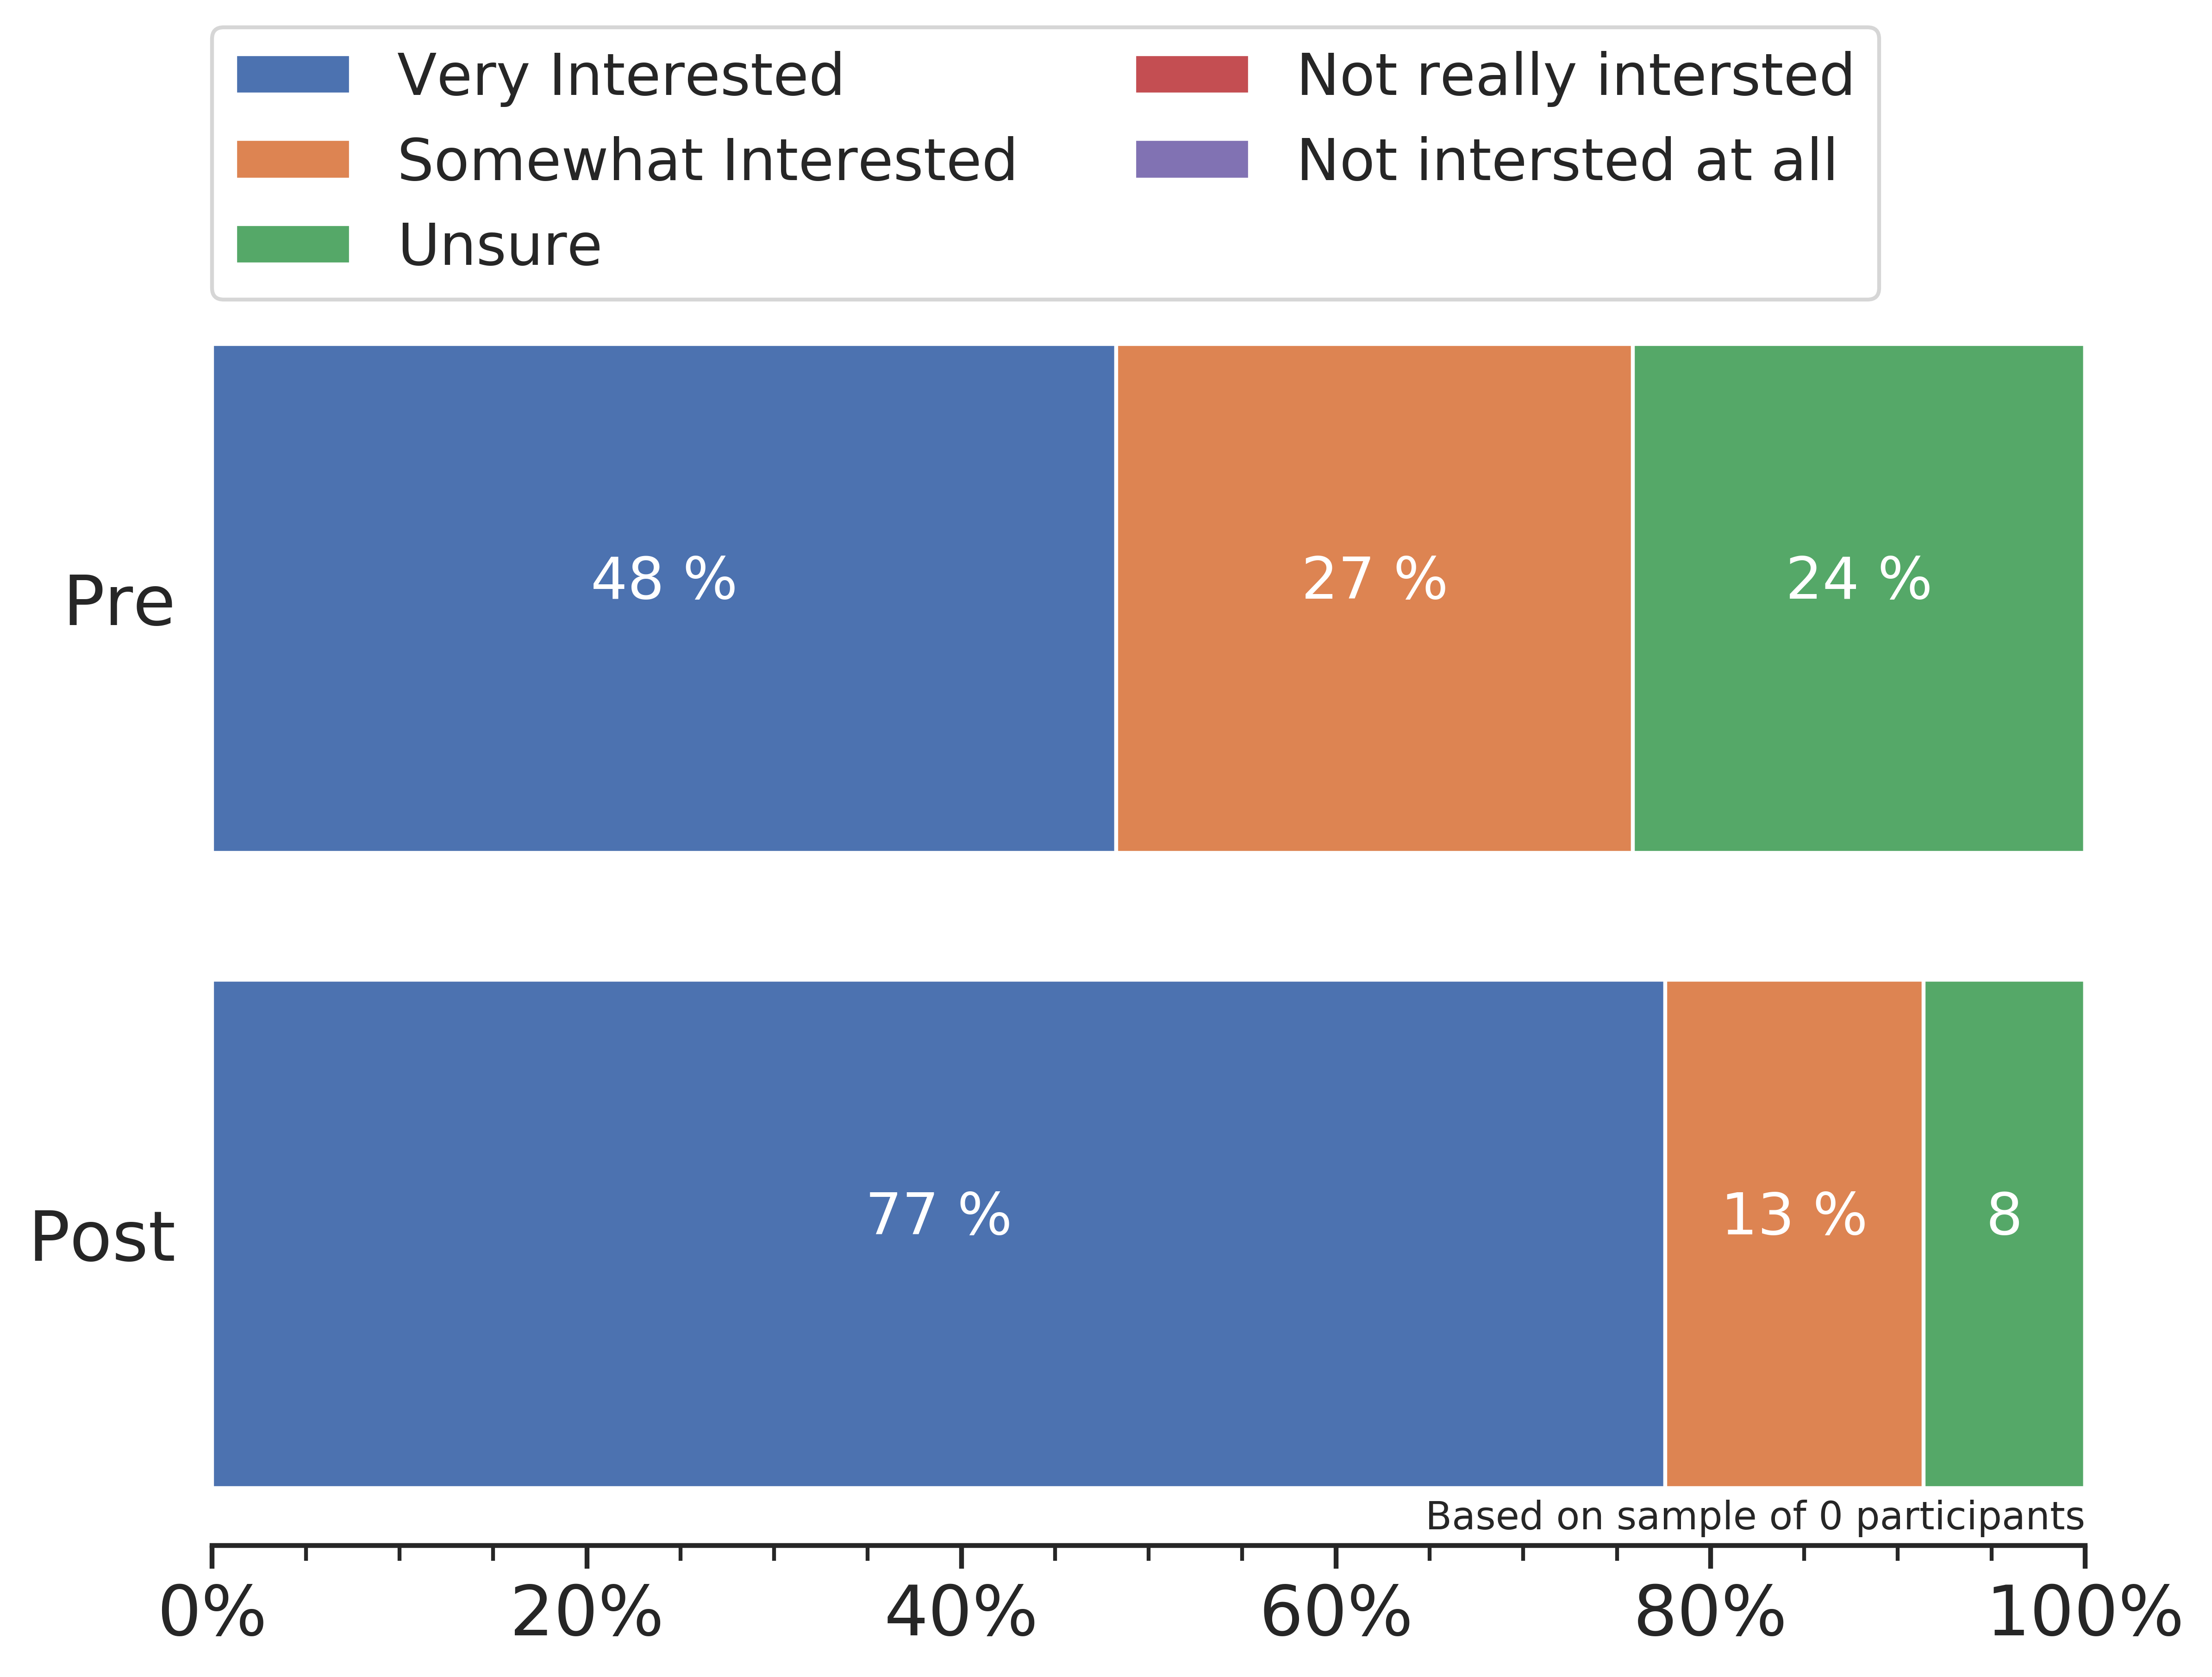
\includegraphics[width=0.85\textwidth]{bar_codinginterest}
\caption{The \DYB participants were asked before and after the workshop how interested they are in doing coding. The workshops increased their interest in coding.  24 per cent of participants were unsure or not interested in coding, whereas after the workshop this dropped to nine per cent. The proportion of participants who are very interested in doing coding increased from 48 per cent before the workshop to 78 per cent after.}
\label{fig:DYBcodinginterest}
\end{figure*}


\begin{figure*}[t!]
    \centering
        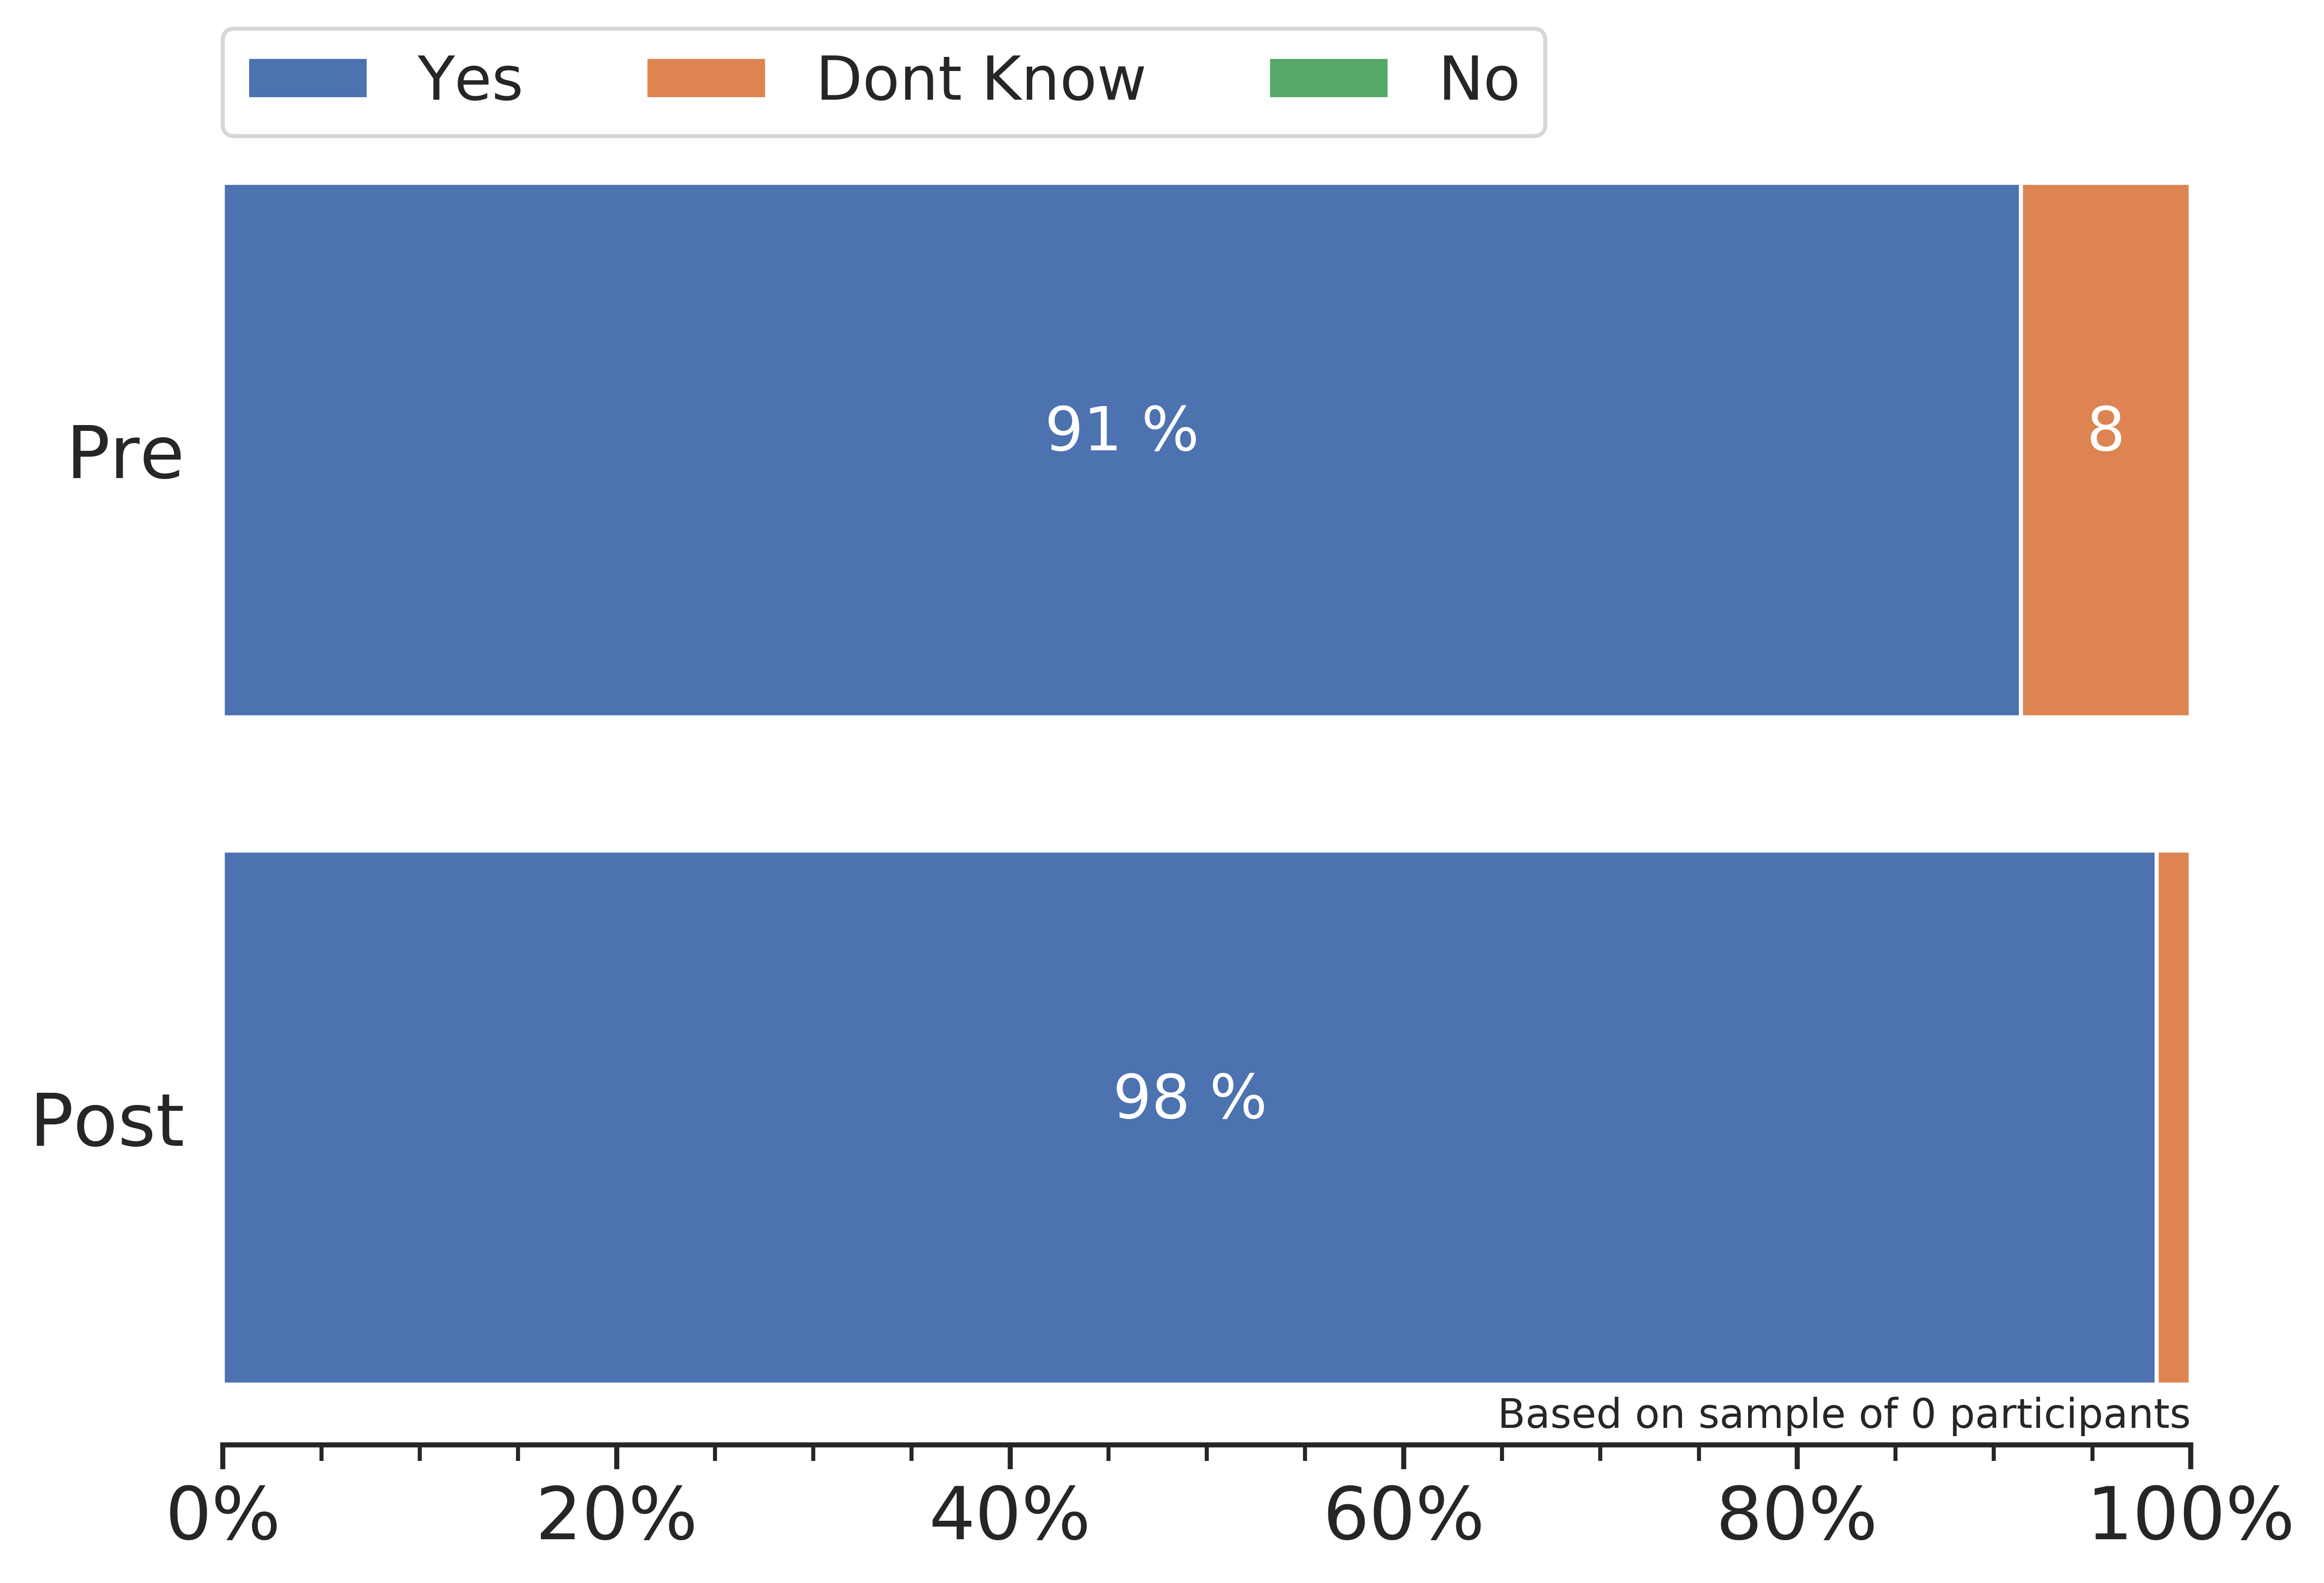
\includegraphics[width=1\textwidth]{bar_techsolve}
\caption{The \DYB participants were asked before and after the workshop whether they believed you can use technology to solve environmental problems. Prior to the workshop there was a high awareness of the potential to use technology to solve problems. The workshop increased this further (from 91 to 98 per cent).} 
\label{fig:techsolve}
\end{figure*}

\begin{figure*}[t!]
    \centering
        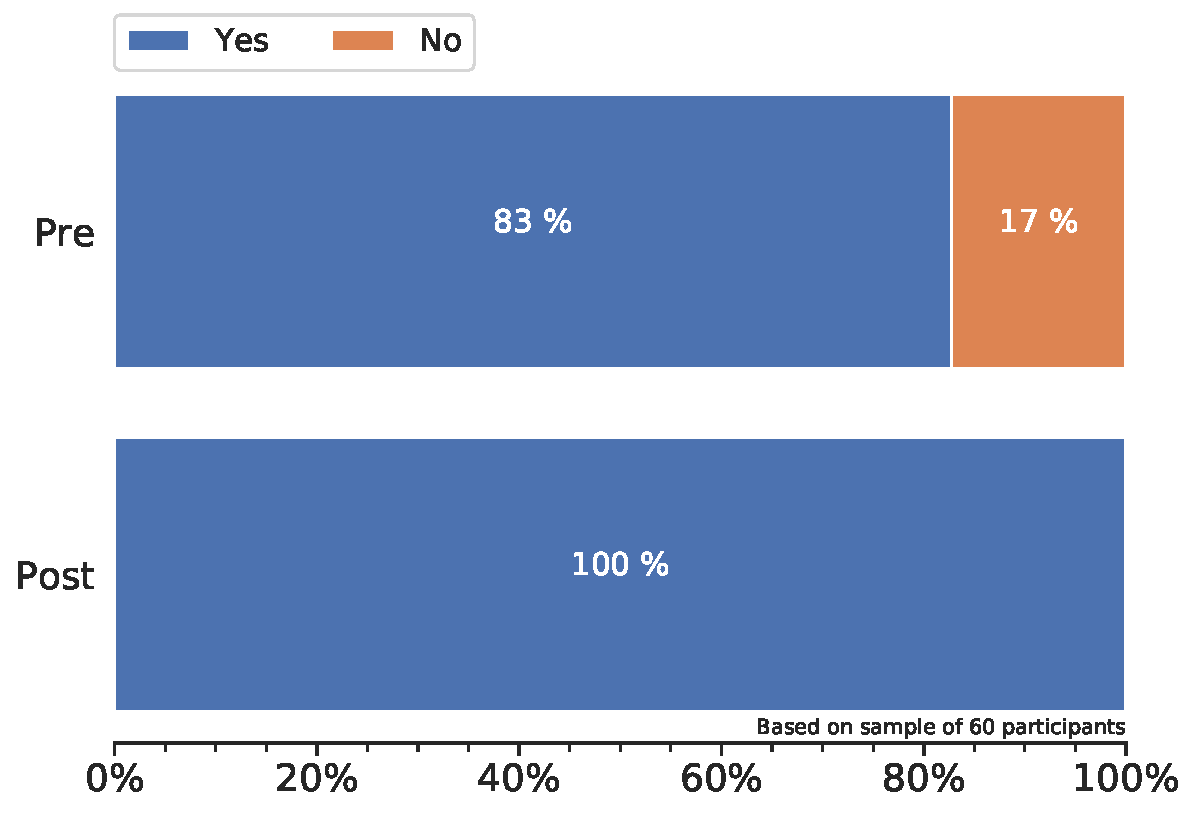
\includegraphics[width=1\textwidth]{bar_knowsdgs}
\caption{The \DYB participants were asked before and after the workshop whether they are familiar with the SDGs. There was an initial high awareness of the SDGs in general amongst the participants, with 83 per cent of participants saying they are have heard of the SDGs prior to the workshop. After the workshop this had increased to 100 per cent. } 
\label{fig:knowsdgs}
\end{figure*}

\begin{figure*}[t!]
    \centering
        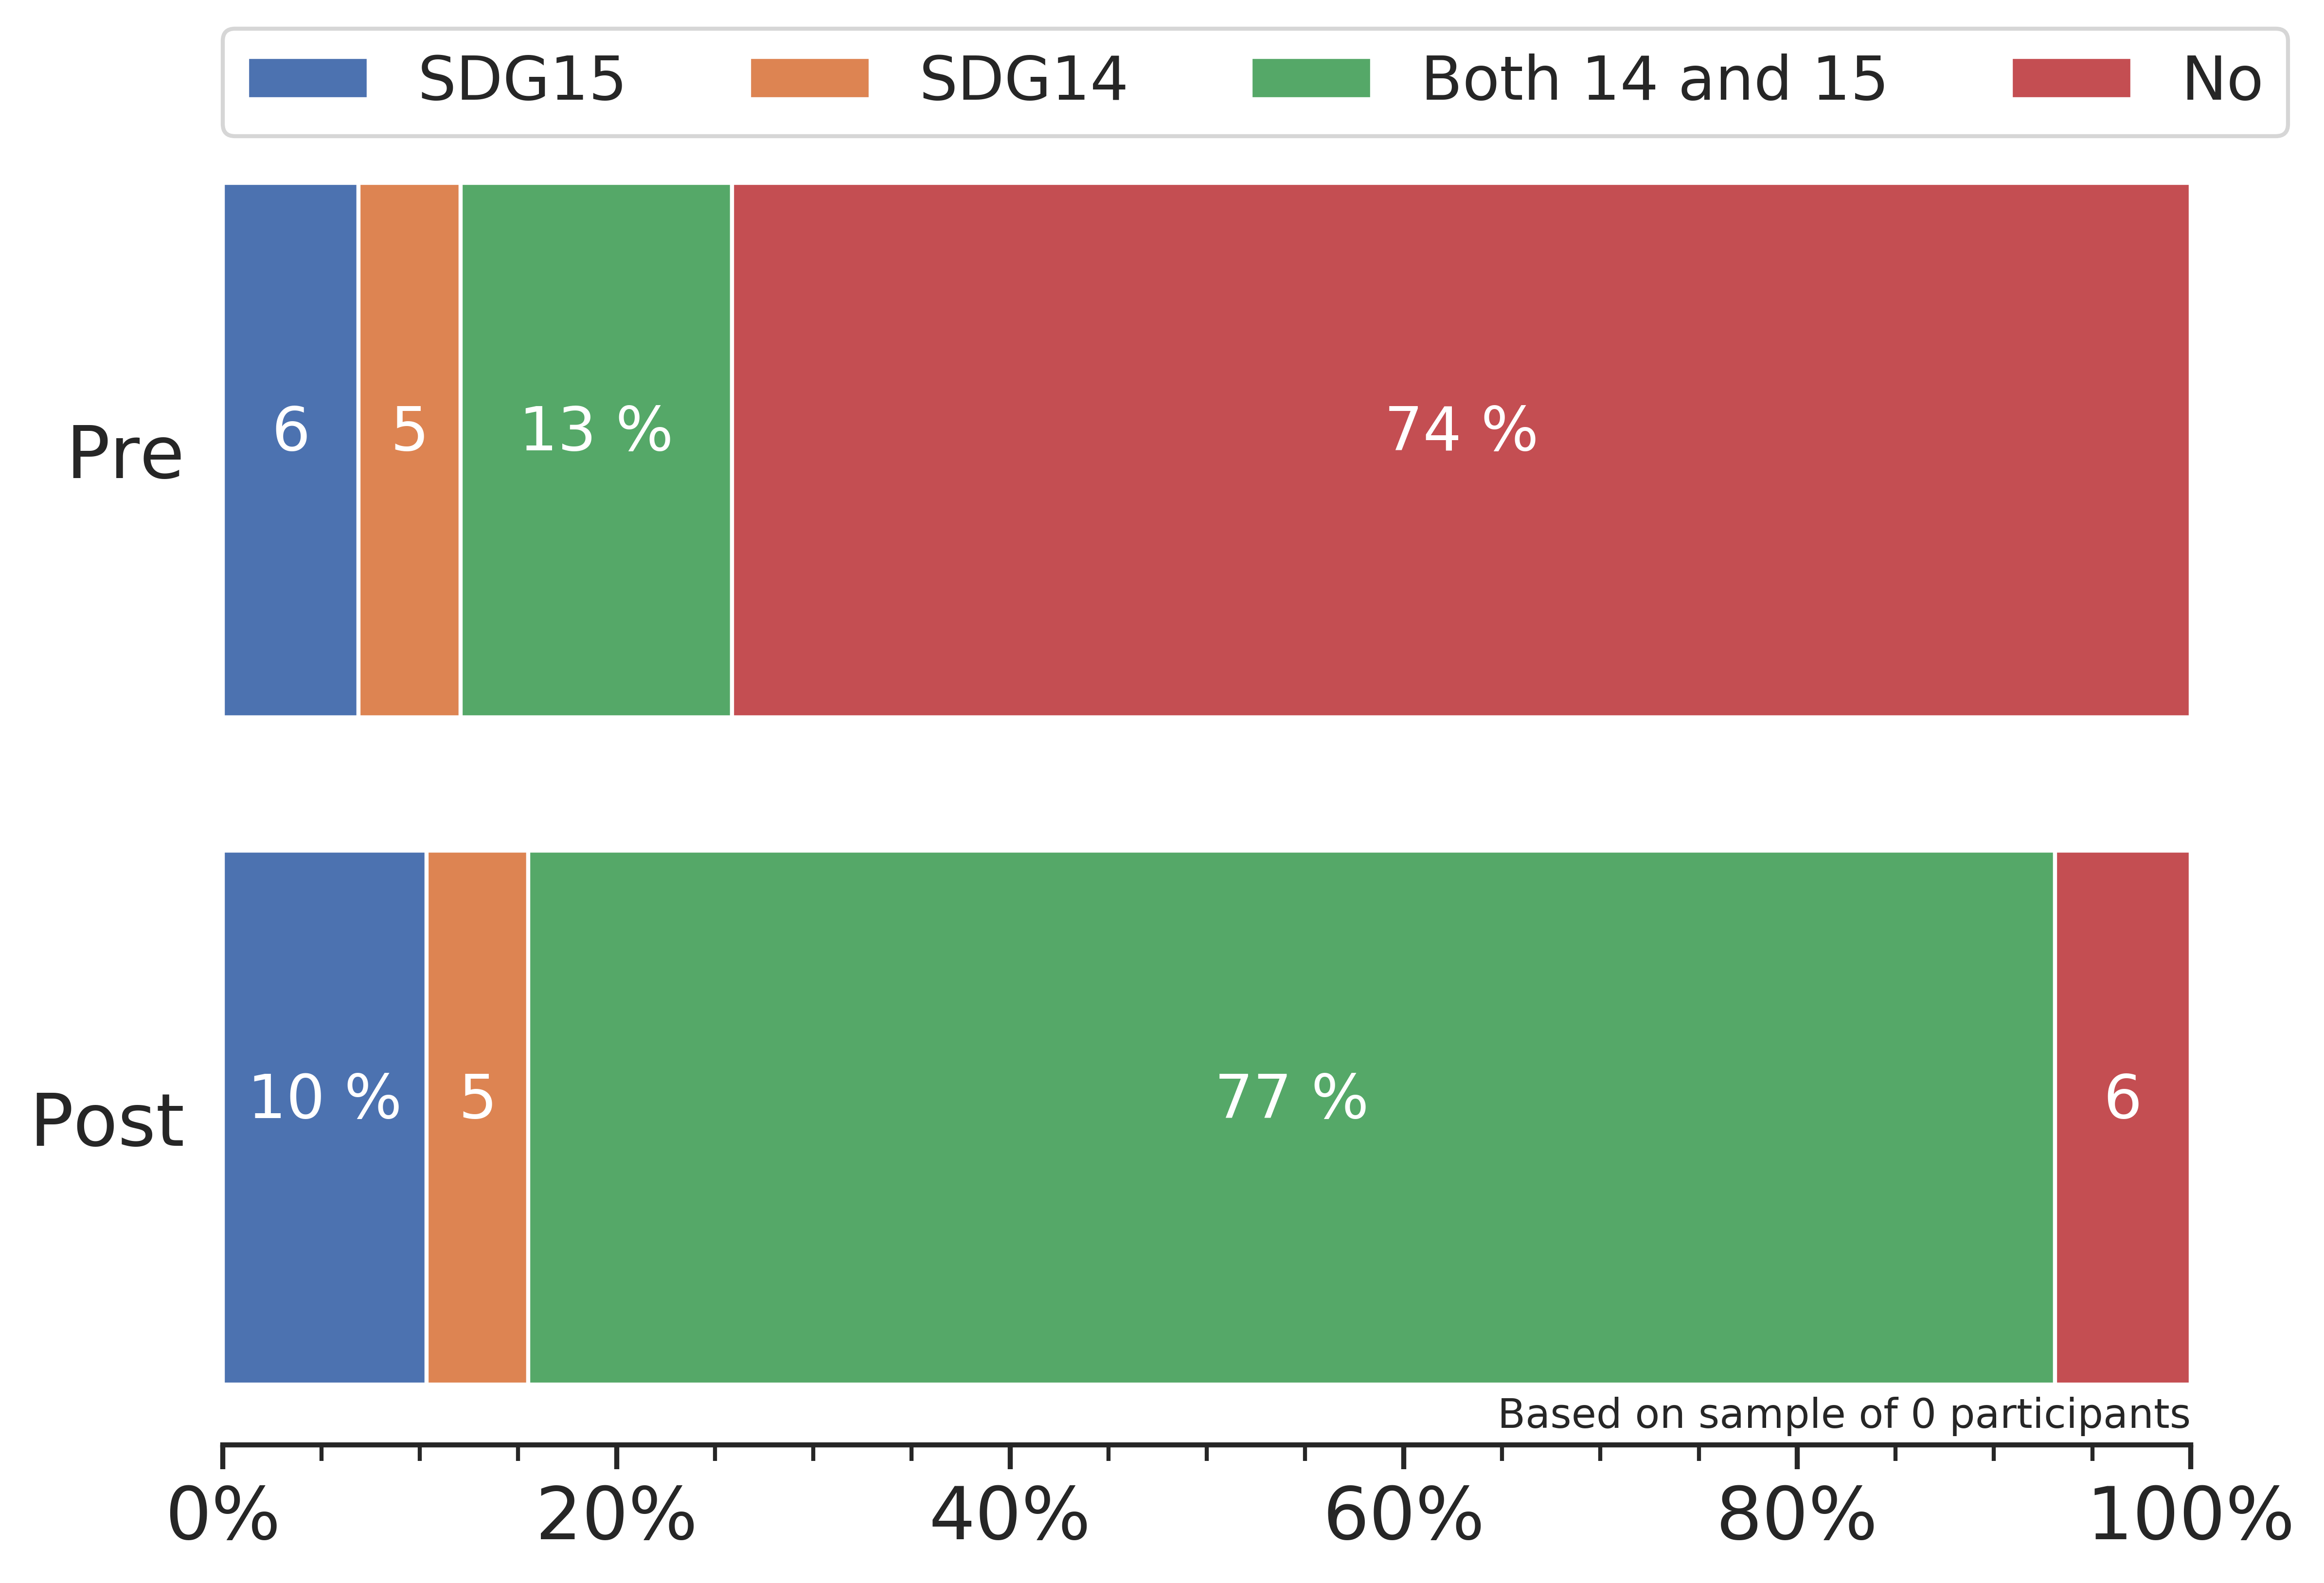
\includegraphics[width=1\textwidth]{bar_knowsdg1415}
\caption{The \DYB participants were asked before and after the workshop whether they are familiar with the SDGs 14 and 15 specifically. Awareness of the specific SDGs 14 and 15 were substantially improved by the workshop. The proportion of participants who said they did not know about either SDG 14 and 15 decreased from 74 per cent before the workshop to seven per cent after the workshop.} 
\label{fig:knowsdg1415}
\end{figure*}

\begin{figure*}[t!]
    \centering
        \includegraphics[width=1\textwidth]{bar_sdgimportant}
\caption{The \DYB participants were asked before and after the workshop how important they felt the SDGs are. The workshop increased the perception of the importance of the SDGs in the participants. After the workshop 84 per cent felt the SDGs are very important compared to 63 per cent before the workshop. The proportion who were unsure or thought they are unimportant decreased from 14 per cent before the workshop to seven per cent after the workshop.} 
\label{fig:sdgimportant}
\end{figure*}


%------------------------------------------------

%\subsubsection{Subsubsection 3} % Sub-sub-section

%\begin{description} % Numbered list example

%\item[First] \hfill \\

%\item[Second] \hfill \\

%\item[Third] \hfill \\

%\end{description} 

%----------------------------------------------------------------------------------------
%	MAJOR SECTION X - TEMPLATE - UNCOMMENT AND FILL IN
%----------------------------------------------------------------------------------------

%\section{Content Section}

%\subsection{Subsection 1} % Sub-section

% Content

%------------------------------------------------

%\subsection{Subsection 2} % Sub-section

% Content

%----------------------------------------------------------------------------------------
%	CONCLUSION
%----------------------------------------------------------------------------------------

%\section{Conclusion} % Major section

%----------------------------------------------------------------------------------------
\chapter{Appendix: Questionnaires}
Here we provide examples of the feedback forms that are used to collect the data shown in this report. Note, that these are in Bengali. 

\begin{figure*}[t!]
    \centering
        \frame{\includegraphics[width=0.98\textwidth]{QuestionnaireP1}}
\caption{An example of the feedback form used with the coding workshop participants. Page 1 of 2. } 
\label{fig:QsP1}
\end{figure*}

\begin{figure*}[t!]
  \ContinuedFloat
  \captionsetup{list=off, format=cont}
    \centering
        \frame{\includegraphics[width=0.98\textwidth]{QuestionnaireP2}}
\caption{An example of the feedback form used with the coding workshop participants. Page 2 of 2. } 
\label{fig:QsP2}
\end{figure*}

\begin{figure*}[t!]
    \centering
        \frame{\includegraphics[width=0.98\textwidth]{Questionnaire_DoYourBit_Pre_bengali}}
\caption{An example of the 'Do Your Bit' workshop questionnaires. Page 1 of 2. } 
\label{fig:QsP1}
\end{figure*}

\begin{figure*}[t!]
  \ContinuedFloat
  \captionsetup{list=off, format=cont}
    \centering
        \frame{\includegraphics[width=0.98\textwidth]{Questionnaire_DoYourBit_Post_bengali}}
\caption{An example of the 'Do Your Bit' workshop questionnaires. Page 2 of 2. } 
\label{fig:QsP2}
\end{figure*}

\end{document}


%\begin{wrapfigure}{l}{0.4\textwidth} % Inline image example
%  \begin{center}
%    \includegraphics[width=0.38\textwidth]{pie_gender}
%  \end{center}
%  \caption{Fish}\label{fig:gender}
%\end{wrapfigure}



%------------------------------------------------

%\subsubsection{Subsubsection 3} % Sub-sub-section

%\begin{description} % Numbered list example

%\item[First] \hfill \\

%\item[Second] \hfill \\

%\item[Third] \hfill \\

%\end{description} 

%----------------------------------------------------------------------------------------
%	MAJOR SECTION X - TEMPLATE - UNCOMMENT AND FILL IN
%----------------------------------------------------------------------------------------

%\section{Content Section}

%\subsection{Subsection 1} % Sub-section

% Content

%------------------------------------------------

%\subsection{Subsection 2} % Sub-section

% Content

%----------------------------------------------------------------------------------------
%	CONCLUSION
%----------------------------------------------------------------------------------------

%\section{Conclusion} % Major section

%----------------------------------------------------------------------------------------


%\begin{wrapfigure}{l}{0.4\textwidth} % Inline image example
%  \begin{center}
%    \includegraphics[width=0.38\textwidth]{pie_gender}
%  \end{center}
%  \caption{Fish}\label{fig:gender}
%\end{wrapfigure}
